\documentclass[11pt,a4paper]{ctexart}
 
% 页面设置
\usepackage[margin=2.5cm]{geometry}
 
% 数学
\usepackage{amsmath,amssymb,amsthm}
\usepackage{mathtools}
\usepackage{bm}
 
% 表格和图形
\usepackage{booktabs}
\usepackage{array}
\usepackage{graphicx}
 
% 代码
\usepackage{listings}
\usepackage{xcolor}
 
% 超链接
\usepackage{hyperref}
\hypersetup{colorlinks=true,linkcolor=blue,citecolor=blue}
 
% 定理环境
\newtheorem{theorem}{定理}[section]
\newtheorem{lemma}[theorem]{引理}
\newtheorem{definition}[theorem]{定义}
\newtheorem{corollary}[theorem]{推论}
\newtheorem{proposition}[theorem]{命题}
 
\theoremstyle{definition}
\newtheorem{example}[theorem]{例}
 
\theoremstyle{remark}
\newtheorem{remark}[theorem]{注}
 
% 代码样式
\lstset{
    language=Python,
    basicstyle=\ttfamily\small,
    keywordstyle=\color{blue},
    commentstyle=\color{gray},
    stringstyle=\color{red},
    numbers=left,
    numberstyle=\tiny\color{gray},
    frame=single,
    breaklines=true,
    breakatwhitespace=true,
    tabsize=4,
    showstringspaces=false
}
 
\usepackage{tikz}
\usetikzlibrary{arrows.meta, calc, positioning, shapes.geometric}
 
\usepackage{tcolorbox}
\tcbuselibrary{most}
 
% 定义颜色
\definecolor{myblue}{RGB}{0, 119, 204}
\definecolor{myred}{RGB}{204, 0, 0}
\definecolor{mygreen}{RGB}{0, 153, 76}
 
% 自定义框
\newtcolorbox{keyinsight}{
    colback=blue!5!white,
    colframe=blue!60!black,
    title=\textbf{关键洞察},
    fonttitle=\bfseries,
    breakable
}
 
\newtcolorbox{warning}{
    colback=red!5!white,
    colframe=red!60!black,
    title=\textbf{注意},
    fonttitle=\bfseries,
    breakable
}
 
\newtcolorbox{recipe}{
    colback=green!5!white,
    colframe=green!50!black,
    title=\textbf{实操要点},
    fonttitle=\bfseries,
    breakable
}
 
\usepackage{pgfplots}
\pgfplotsset{compat=1.18}
\usepgfplotslibrary{groupplots}
 
\usepackage{enumitem}
 
% 简写宏
\newcommand{\RMS}{\mathrm{RMS}}
\newcommand{\E}{\mathbb{E}}
\newcommand{\Var}{\mathrm{Var}}
\newcommand{\msign}{\mathrm{msign}}
\newcommand{\bigT}{\Theta}
 
% 标题
\title{\textbf{优化算法：从理论到大规模实践} \\ \Large 第8周讲义：优化器尺度规律与随机化算法}
\author{}
\date{}
 
\begin{document}
 
\maketitle
\tableofcontents
\newpage
 

\part{优化器的尺度规律：RMS 对齐与 MuP}
%%%%%%%%%%%%%%%%%%%%%%%%%%%%%%%%%%%%%%%%%%%%%%%%%%%%%%%%%%%%%%%%%%%%%%%%%%%%%%%
 
\section{开场：两个"数字奇迹"}
 
训练大 LLM 时人们反复观察到两个非常稳定、几乎与数据无关的现象：
 
\begin{enumerate}
    \item \textbf{Update RMS $\approx 0.2$}：Warmup 结束后 AdamW 的 update 向量 $\bm{u}_t = \bm{m}_t/\sqrt{\bm{v}_t}$ 的 RMS 稳定在 0.2--0.3，无论模型多大、数据是什么。
    \item \textbf{Weight RMS $\approx \sqrt{\eta/(2\lambda)}$}：训出来的模型权重 RMS 只由学习率 $\eta$ 和 weight decay $\lambda$ 决定。
\end{enumerate}
 
这两个现象背后藏着一整套跨优化器、跨模型尺度的超参数迁移规律——正是本 Part 的主角。
 
\textbf{为什么重要？}完整训练一次大型 LLM 的成本是昂贵的，我们不可能在大模型上反复试超参数。如果能在小模型上仔细搜索超参、然后按照某个缩放规律迁移到大模型，就能节省大量算力。这就是 Kimi K2 的"Match Adam Update RMS"技巧（对齐不同优化器）、以及 MuP（对齐不同尺度）做的事情。
 
本 Part 的逻辑链：
\begin{center}
\textbf{Update RMS 的平均场推导} $\to$ \textbf{Weight RMS} $\to$ \textbf{Muon 超参迁移} \\
$\to$ \textbf{MuP 四条件推导} $\to$ \textbf{谱条件：MuP 的高阶版}
\end{center}
 
\begin{keyinsight}
贯穿全 Part 的元思想：\textbf{高维 + 平均场 = 可预测的渐近规律}。
\begin{itemize}
    \item 优化器的稳态 RMS 可以用几何级数求和 + 方差可加性算出来；
    \item 跨模型尺度的学习率规律可以用谱范数不等式代数地推出来；
    \item 不依赖分布假设，只依赖矩阵结构的尺度。
\end{itemize}
这套思想和 Part 2 的 JL 引理、MP 分布完全同源——高维随机是朋友，不是敌人。
\end{keyinsight}
 
% ============================================================
\section{AdamW 的状态变量}
 
\subsection{更新规则}
 
AdamW 在每一步迭代中维护并更新以下状态：
\begin{align}
\bm{m}_t &= \beta_1 \bm{m}_{t-1} + (1-\beta_1)\bm{g}_t \\
\bm{v}_t &= \beta_2 \bm{v}_{t-1} + (1-\beta_2)\bm{g}_t^2 \\
\bm{u}_t &= \bm{m}_t \big/ \sqrt{\bm{v}_t} \\
\bm{\theta}_t &= \bm{\theta}_{t-1} - \eta\bigl(\bm{u}_t + \lambda\bm{\theta}_{t-1}\bigr)
\end{align}
 
所有乘除、平方、开方均为逐元素（Hadamard）运算。$t\to\infty$ 时 bias correction 可以忽略（$\beta_1^t, \beta_2^t \to 0$）。
 
\subsection{\texorpdfstring{每个变量的含义：$\bm{g}, \bm{m}, \bm{v}, \bm{u}$}{每个变量的含义}}
 
\textbf{$\bm{m}_t$（一阶矩 EMA，动量）}：梯度 $\bm{g}_t$ 的指数滑动平均
\[ \bm{m}_t = (1-\beta_1)\sum_{i=1}^t \beta_1^{t-i}\, \bm{g}_i \]
估计 $\E[\bm{g}]$，$\beta_1 = 0.9$ 对应约 10 步的有效窗口。
 
\textbf{$\bm{v}_t$（二阶矩 EMA）}：逐元素梯度平方的 EMA
\[ \bm{v}_t = (1-\beta_2)\sum_{i=1}^t \beta_2^{t-i}\, \bm{g}_i^2 \]
估计 $\E[\bm{g}^2] = \bm{\mu}^2 + \bm{\sigma}^2$。$\sqrt{\bm{v}_t}$ 可解释为"每个参数方向上梯度的典型尺度"。$\beta_2 = 0.95$ 对应更长的窗口（约 20 步），因为分母需要更平滑。
 
\textbf{$\bm{u}_t = \bm{m}_t/\sqrt{\bm{v}_t}$（Adam 的灵魂）}：自适应的坐标归一化
\begin{itemize}
    \item 分子 $\bm{m}_t$ 提供梯度的\emph{方向}（信号分量）；
    \item 分母 $\sqrt{\bm{v}_t}$ 提供梯度的\emph{尺度}（大小分量）；
    \item 两者相除 $\Longrightarrow$ 对每个参数独立做归一化；
    \item 净效果：\textbf{所有参数方向的 update 尺度被拉至同一量级}。
\end{itemize}
 
\begin{center}
\renewcommand{\arraystretch}{1.3}
\begin{tabular}{llllc}
\toprule
变量 & 维度 & 估计对象 & 稳态期望 & 作用 \\
\midrule
$\bm{g}_t$ & $\mathbb{R}^d$ & --- & $\bm{\mu}$ & 当前梯度 \\
$\bm{m}_t$ & $\mathbb{R}^d$ & $\E[\bm{g}]$ & $\bm{\mu}$ & 方向（信号） \\
$\bm{v}_t$ & $\mathbb{R}^d$ & $\E[\bm{g}^2]$ & $\bm{\mu}^2 + \bm{\sigma}^2$ & 尺度（归一化） \\
$\bm{u}_t$ & $\mathbb{R}^d$ & $\bm{m}_t / \sqrt{\bm{v}_t}$ & $\|\cdot\|_\RMS \approx 0.23$ & 实际更新 \\
\bottomrule
\end{tabular}
\end{center}
 
\begin{warning}
AdamW 中所有涉及 $\bm{g}, \bm{m}, \bm{v}$ 的运算都是\textbf{逐元素的}，不是向量内积或矩阵模长。这也是为什么整个理论推导用 $\|\cdot\|_\RMS$ 而非 $\|\cdot\|_2$ 作为度量——RMS 与逐元素运算自然匹配。
\end{warning}
 
% ============================================================
\section{数值模拟先行：建立对 0.2 的信心}
 
教学哲学：\textbf{先让学生相信现象，再推公式}。下面用 20 行 Python 直接模拟 AdamW 在纯噪声梯度下的行为：
 
\begin{lstlisting}
import numpy as np
 
N, T = 10000, 2000
beta1, beta2 = 0.9, 0.95
m, v = 0, 0
for t in range(1, T + 1):
    g = np.random.randn(N)          # 纯噪声梯度！
    m = beta1 * m + (1 - beta1) * g
    v = beta2 * v + (1 - beta2) * g**2
    u = m / v**0.5
 
rms = (u**2).mean()**0.5
print(rms)                          # ≈ 0.2294
\end{lstlisting}
 
\begin{keyinsight}
梯度用的是\textbf{纯噪声} $\mathcal{N}(0, I)$，居然得到和真实 LLM 训练几乎一样的 0.23！这反过来表明：实际训练中单步梯度的信噪比很低，\textbf{噪声近似就足以捕捉 update RMS 的主导行为}。
\end{keyinsight}
 
让学生自己改动代码后，可以观察到：
\begin{itemize}
    \item Update RMS 对 $\beta_1$ 敏感；
    \item 对 $\beta_2$ 几乎不敏感；
    \item 非零梯度均值（增大梯度信噪比）会让 RMS 变大。
\end{itemize}
 
现在有了可验证的目标，我们可以上公式。
 
% ============================================================
\section{Update RMS 的平均场推导}
 
\subsection{核心技巧：平均场分离期望}
 
$t\to\infty, \epsilon\to 0$ 的稳态下 $\bm{u}_t = \bm{m}_t/\sqrt{\bm{v}_t}$。我们要算 $\E[\bm{u}_t^2]$，做如下\textbf{平均场近似}：
\begin{equation}
\E\!\left[\frac{\bm{m}_t^2}{\bm{v}_t}\right] \approx \frac{\E[\bm{m}_t^2]}{\E[\bm{v}_t]}.
\label{eq:meanfield}
\end{equation}
 
\begin{remark}
这一步严格意义上是错的——$\E[X/Y] \ne \E[X]/\E[Y]$。但这是平均场近似的灵魂：\textbf{先算，合理就好}，事后与模拟对比验证。前一节的数值模拟已经证实这个近似在 $\beta_2 \geq 0.9$ 时极为准确。
\end{remark}
 
设 $\E[\bm{g}] = \bm{\mu}$，$\Var[\bm{g}] = \bm{\sigma}^2$，故 $\E[\bm{g}^2] = \bm{\mu}^2 + \bm{\sigma}^2$。
 
\subsection{分母的计算}
 
\begin{align}
\E[\bm{v}_t] 
&= (1-\beta_2) \sum_{i=1}^{t} \beta_2^{t-i}\, \E[\bm{g}_i^2] \notag \\
&= (1-\beta_2)(\bm{\mu}^2 + \bm{\sigma}^2) \sum_{i=1}^{t} \beta_2^{t-i} \notag \\
&= (1 - \beta_2^t)(\bm{\mu}^2 + \bm{\sigma}^2) \notag \\
&\xrightarrow{t \to \infty} \bm{\mu}^2 + \bm{\sigma}^2.
\label{eq:Ev}
\end{align}
 
\subsection{分子的计算}
 
利用 $\E[\bm{m}_t^2] = \E[\bm{m}_t]^2 + \Var[\bm{m}_t]$：
 
\textbf{均值部分}（同样 EMA 几何级数）：$\E[\bm{m}_t] \to \bm{\mu}$。
 
\textbf{方差部分}（独立随机变量方差的平方可加性）：
\begin{align}
\Var[\bm{m}_t] 
&= (1-\beta_1)^2 \sum_{i=1}^{t} \beta_1^{2(t-i)}\, \bm{\sigma}^2 \notag \\
&= (1-\beta_1)^2 \cdot \frac{1 - \beta_1^{2t}}{1 - \beta_1^2}\, \bm{\sigma}^2 \notag \\
&\xrightarrow{t \to \infty} \frac{(1-\beta_1)^2}{1-\beta_1^2}\, \bm{\sigma}^2
= \frac{1-\beta_1}{1+\beta_1}\, \bm{\sigma}^2.
\label{eq:Varm}
\end{align}
 
合并：
\begin{equation}
\E[\bm{m}_t^2] \approx \bm{\mu}^2 + \frac{1-\beta_1}{1+\beta_1}\, \bm{\sigma}^2.
\end{equation}
 
\subsection{主结果：Update RMS 渐近公式}
 
代入 \eqref{eq:meanfield}、\eqref{eq:Ev}、\eqref{eq:Varm}：
\begin{equation}
\boxed{\;
\|\bm{u}_t\|_\RMS \approx \sqrt{\frac{\|\bm{\mu}\|^2/\|\bm{\sigma}\|^2 + \frac{1-\beta_1}{1+\beta_1}}{\|\bm{\mu}\|^2/\|\bm{\sigma}\|^2 + 1}}.
\;}
\label{eq:urms-general}
\end{equation}
 
\begin{theorem}[零均值特例——核心公式]
假设梯度 $\bm{g}_t$ 零均值，即 $\bm{\mu} = 0$。则 $t \to \infty$ 稳态下：
\begin{equation}
\|\bm{u}_t\|_\RMS \approx \sqrt{\frac{1-\beta_1}{1+\beta_1}}.
\end{equation}
特别地，代入 $\beta_1 = 0.9$：$\|\bm{u}_t\|_\RMS \approx \sqrt{0.1/1.9} \approx 0.2294$。
\end{theorem}
 
\begin{keyinsight}
公式的三个惊人性质：
\begin{enumerate}
    \item \textbf{不含 $\beta_2$}——与模拟观察一致；
    \item \textbf{不含 $t$}（稳态）；
    \item \textbf{不含数据}——仅由超参 $\beta_1$ 决定。
\end{enumerate}
\end{keyinsight}
 
% ============================================================
\section{Weight RMS 的推导}
 
\subsection{关键视角转换：Weight Decay 是 Update 的 EMA}
 
令 $\beta_3 \triangleq 1 - \eta\lambda$，AdamW 的权重更新可改写为：
\begin{equation}
\bm{\theta}_t = \beta_3 \bm{\theta}_{t-1} + (1-\beta_3)\!\left(-\frac{\bm{u}_t}{\lambda}\right).
\label{eq:theta-ema}
\end{equation}
 
\begin{keyinsight}
Weight decay 本质上\textbf{不是在"惩罚"权重}，而是\textbf{对更新量 $-\bm{u}_t/\lambda$ 做 EMA}。$\beta_3$ 扮演了类似 $\beta_1, \beta_2$ 的 EMA 衰减因子角色。这个视角转换是 scaling law 系列工作（Wang 等 2024、Bergsma 等 2024）的理论支点。
\end{keyinsight}
 
\subsection{快速估计：利用高维正交性}
 
对 \eqref{eq:theta-ema} 两边取 $\|\cdot\|_\RMS^2$，高维空间中随机向量近似正交，故 $\bm{\theta}_{t-1} \cdot \bm{u}_t \approx 0$。稳态下 $\|\bm{\theta}_t\|_\RMS = \|\bm{\theta}_{t-1}\|_\RMS$：
\begin{equation}
(1 - \beta_3^2) \|\bm{\theta}_t\|_\RMS^2 \approx (1-\beta_3)^2 \|\bm{u}_t\|_\RMS^2 / \lambda^2.
\end{equation}
 
利用 $\beta_3 \approx 1$ 时 $1 - \beta_3^2 \approx 2(1-\beta_3)$：
\begin{equation}
\|\bm{\theta}_t\|_\RMS \approx \sqrt{\frac{1-\beta_1}{1+\beta_1}} \cdot \sqrt{\frac{\eta}{2\lambda}}.
\label{eq:theta-fast}
\end{equation}
 
\subsection{更精细：二次平均场}
 
快速估计的误差来自 $\bm{\theta}_{t-1} \cdot \bm{u}_t \approx 0$ 并不严格成立。更精细地，对 $\bm{u}_t$ 再做一层 EMA 平均，展开到单步梯度 $\bm{g}_i$ 层级。经过化简，在 $\bm{\mu} = 0$、$t \to \infty$ 下得到：
 
\begin{theorem}[Weight RMS 的精细渐近——第二核心公式]
\begin{equation}
\boxed{\;
\|\bm{\theta}_t\|_\RMS \approx \sqrt{\frac{\eta}{2\lambda}}.
\;}
\label{eq:theta-main}
\end{equation}
\end{theorem}
 
\begin{keyinsight}
公式 \eqref{eq:theta-main} \textbf{连 $\beta_1$ 都消掉了}！为什么？因为 weight decay 的长时间 EMA 又把动量效应平均了一次——\textbf{两次平均抵消了所有 $\beta_1$ 相关的一阶项}。稳态下，weight RMS 只依赖 $\eta$ 和 $\lambda$ 这对最基本的超参。
\end{keyinsight}
 
\subsection{一般结果与极限情形}
 
完整的一般公式（允许非零均值、有限 $t$、非零初始权重）：
\begin{equation}
\|\bm{\theta}_t\|_\RMS^2 \approx \beta_3^{2t} \|\bm{\theta}_0\|_\RMS^2 
+ (1-\beta_3^t)^2 \cdot \frac{\|\bm{\mu}\|^2/\|\bm{\sigma}\|^2 + \frac{(1-\beta_3)(1+\beta_3^t)}{2(1-\beta_3^t)}}{\lambda^2(\|\bm{\mu}\|^2/\|\bm{\sigma}\|^2 + 1)}.
\end{equation}
 
两个有意思的极限：
 
\begin{example}[无 weight decay]
$\lambda \to 0$：$\|\bm{\theta}_t\|_\RMS^2 \approx \|\bm{\theta}_0\|_\RMS^2 + \eta^2 t$，按 $\eta\sqrt{t}$ 增长。这意味着没有 weight decay 时，可以通过 learning rate schedule 控制 weight RMS 的稳定性。
\end{example}
 
\begin{example}[SignSGDM 版本]
$\Delta\bm{W} = -\eta\, \mathrm{sign}(\bm{m}_t) = -\eta\, \bm{m}_t/\sqrt{\bm{m}_t^2}$。类似推导给出：
\[
\|\bm{\theta}_t\|_\RMS \approx \sqrt{\frac{\eta}{2\lambda} \cdot \frac{1+\beta_1}{1-\beta_1}}.
\]
即 SignSGDM 的 weight RMS 是 AdamW 的 $\sqrt{(1+\beta_1)/(1-\beta_1)}$ 倍。
\end{example}
 
% ============================================================
\section{应用：Muon 与 AdamW 的超参迁移}
 
上面解决了"同一个优化器内部的尺度规律"。现在把结论用到\textbf{不同优化器之间的迁移}——这正是 Kimi K2 训练中使用的"Match Adam Update RMS"技巧。
 
\subsection{Muon 的结构分析}
 
Kimi 版 Muon 的更新规则（$\bm{W} \in \mathbb{R}^{m \times n}$）：
\begin{align}
\bm{M}_t &= \mu \bm{M}_{t-1} + \bm{G}_t \\
\bm{O}_t &= \msign(\bm{M}_t) \cdot \sqrt{\max(n, m)} \cdot 0.2 \\
\bm{W}_t &= \bm{W}_{t-1} - \eta_t(\bm{O}_t + \lambda \bm{W}_{t-1})
\end{align}
其中 $\msign(\cdot)$ 通过 Newton-Schulz 迭代近似矩阵符号函数，把所有奇异值归一到 1。
 
\subsection{\texorpdfstring{逐步拆解 $\msign$ 的 RMS}{逐步拆解 msign 的 RMS}}
 
让学生自己完成：
\begin{itemize}
    \item $\msign(\bm{M})$ 的所有奇异值 $= 1$；
    \item 因此 $\|\msign(\bm{M})\|_F = \sqrt{\min(m, n)}$；
    \item Per-element RMS $= \sqrt{\min(m,n)/(mn)} = 1/\sqrt{\max(m,n)}$。
\end{itemize}
 
所以 Kimi Muon 的设计逻辑是：
\begin{enumerate}
    \item 乘 $\sqrt{\max(m,n)}$ $\Longrightarrow$ 把 RMS 归一到 $1$；
    \item 再乘 $0.2$ $\Longrightarrow$ 对齐到 AdamW 的 Update RMS。
\end{enumerate}
 
\subsection{迁移定理}
 
\begin{theorem}[超参数迁移]
由于 Weight RMS 公式 \eqref{eq:theta-main} \textbf{只依赖 Update RMS 与 $\eta, \lambda$}，而不依赖优化器的具体动量结构：
\[
\text{对齐 Update RMS} \quad \Longrightarrow \quad \text{可直接复用 } \eta, \lambda.
\]
\end{theorem}
 
这就是迁移的"自由午餐"——AdamW 训练得到的最优 $\eta, \lambda$ 可以直接用于 Muon 训练。
 
\subsection{进阶视角：Total Update Contribution}
 
另一个对齐视角来自 Rotational Equilibrium 论文。在稳态下，单步梯度 $\bm{g}_t$ 对未来所有步的\textbf{总贡献}是：
\begin{equation}
\sum_{i=0}^{\infty} \beta_1^i (1-\beta_1) \bm{g}_t = \bm{g}_t.
\end{equation}
即单步梯度的总效应\textbf{与 $\beta_1$ 无关}——$\beta_1$ 只是把效应在时间上摊平。从 TUC 视角：
\begin{itemize}
    \item AdamW 的 TUC $\propto \eta_t \sqrt{mn}$；
    \item Muon (Kimi) 的 TUC $\approx 1.25\, \eta_t \sqrt{\min(n,m)} \cdot \sqrt{\max(n,m)} = 1.25\, \eta_t \sqrt{mn}$。
\end{itemize}
其中 $1.25 \approx 0.2 \times \sqrt{(1+\mu)/(1-\mu)}|_{\mu=0.95}$。\textbf{TUC 对齐与 RMS 对齐给出的 $0.2$ 这个倍数异曲同工。}
 
\begin{remark}
两个视角在此渐近等价，但在"最优学习率是否随 $\beta_1$ 变化"这个问题上有细微分歧。这是一个开放的实验问题，适合作为期末研究课题。
\end{remark}
 
\subsection{速查表}
 
\begin{center}
\renewcommand{\arraystretch}{1.5}
\begin{tabular}{lll}
\toprule
量 & 渐近值（零均值稳态） & 依赖超参 \\
\midrule
Update RMS (AdamW) & $\sqrt{(1-\beta_1)/(1+\beta_1)} \approx 0.23$ & 仅 $\beta_1$ \\
Update RMS (SignSGDM) & $\sqrt{(1+\beta_1)/(1-\beta_1)} \times \text{AdamW}$ & 仅 $\beta_1$ \\
Weight RMS (AdamW) & $\sqrt{\eta/(2\lambda)}$ & 仅 $\eta, \lambda$ \\
Weight RMS (Muon-Kimi) & $\sqrt{\eta/(2\lambda)}$（对齐后） & 仅 $\eta, \lambda$ \\
\bottomrule
\end{tabular}
\end{center}
 
% ============================================================
\section{MuP：超参数跨模型尺度的迁移规律}
 
上面解决了"优化器之间迁移"的问题。现在解决"\textbf{模型尺度之间迁移}"——在小模型上搜索的最优学习率如何迁移到大模型？这就是 MuP（Maximal Update Parametrization）。
 
\subsection{Motivation 与方法大意}
 
MuP 研究的是\textbf{超参数随模型尺度（主要是宽度 $d$）的变化规律}。请注意：
 
\begin{warning}
MuP \textbf{不研究}"什么是最优超参"，只研究"最优超参随尺度的变化规律"。所以我们需要先在某个小模型上搜索最优超参，然后按缩放规律迁移到大模型。
\end{warning}
 
推导原理：\textbf{让前向传播、反向传播、损失增量、特征变化都不随模型尺度发生明显变化}。具体做法是分析初始化阶段的数量级，然后假设结论代表后续优化的规律——"好的开始是成功的一大半"。
 
\subsection{前向传播：初始化尺度规律}
 
考虑线性层 $\bm{Y} = \bm{X}\bm{W}$，$\bm{W} \in \mathbb{R}^{d_\text{in} \times d_\text{out}}$。RMS 作为矩阵尺度指标：
\[
\RMS(\bm{W}) = \sqrt{\frac{1}{d_\text{in} d_\text{out}} \sum_{i,j} W_{i,j}^2}.
\]
 
要使初始化阶段 $\RMS(\bm{X}) \approx \RMS(\bm{Y})$：
 
\begin{proposition}[fan\_in 初始化]
"均值为 0、方差\textbf{正比于} $1/d_\text{in}$"的随机初始化。
\end{proposition}
 
对于非线性层 $\bm{Y} = \phi(\bm{X}\bm{W})$（如 ReLU），Kaiming 初始化与 LeCun 仅差一个尺度无关常数。这给出：
 
\begin{keyinsight}
\textbf{激活函数的影响是模型尺度无关的}。如果只分析模型尺度效应，可以忽略激活函数的存在，直接用 LeCun 初始化的缩放规律 $\propto 1/d_\text{in}$。
\end{keyinsight}
 
\subsection{反向传播的冲突}
 
反向传播给出 $\partial L/\partial \bm{X} \sim (\partial L/\partial \bm{Y}) \bm{W}^\top$，要求 fan\_out 初始化（方差 $\propto 1/d_\text{out}$）。
 
当 $d_\text{in} \neq d_\text{out}$ 时前向与反向要求冲突。折中方案是 Xavier 初始化（fan\_avg）——但两者都没兼顾。更好的办法是\textbf{设计模型让大部分参数都是方阵}。
 
\subsection{损失增量与尺度爆炸}
 
考虑 $\Delta L \approx -\eta \|X^\top \partial L/\partial Y\|_F^2$。分析 $\|X^\top \partial L/\partial Y\|_F^2$：
\begin{itemize}
    \item 是 $d_\text{in} \times d_\text{out}$ 个数的平方和；
    \item 如果前向和反向都稳定，每个元素是 $\bigT(1)$；
    \item 所以是 $\bigT(d_\text{in} d_\text{out})$。
\end{itemize}
 
\begin{warning}
\textbf{学习率不能跨尺度直接使用！}如果直接把小模型的 $\eta$ 用到大模型，$\Delta L$ 会随参数尺度 $d_\text{in} d_\text{out}$ 爆炸——训练过程无法复制，甚至因步子太大无法收敛。
\end{warning}
 
\subsection{标准模型簇}
 
MuP 考虑如下三分结构：
\begin{align*}
\bm{Y}_\text{in} &= \bm{X} \bm{W}_\text{in}, & \bm{W}_\text{in} &\in \mathbb{R}^{d_\text{in} \times d} \\
\bm{Y}_\text{out} &= \text{NN}(\bm{Y}_\text{in}; \Omega), & \bm{W}_k &\in \mathbb{R}^{d \times d}, k=1,\ldots,K \\
\bm{Z} &= \bm{Y}_\text{out} \bm{W}_\text{out}, & \bm{W}_\text{out} &\in \mathbb{R}^{d \times d_\text{out}}
\end{align*}
 
$d_\text{in}, d_\text{out}$ 是任务相关的常数；$d$（hidden size）是可变的。MuP 研究超参随 $d$ 的规律。
 
\begin{remark}
约定方阵是为了简化分析。真正目的是假设 NN 参数里没有尺度无关的形状（不允许 $d\times 64$，但允许 $d \times 4d$）。
\end{remark}
 
\subsection{SGD 下的学习率规律}
 
对 $\bm{W}_\text{in}, \Omega, \bm{W}_\text{out}$ 分别求梯度并分析：
\begin{enumerate}
    \item \textbf{$\bm{W}_\text{out}$}：$\partial L/\partial \bm{W}_\text{out}$ 的 RMS 是 $\bigT(1)$，$\|\cdot\|_F^2$ 是 $d \times d_\text{out}$ 个数平方和 $= \bigT(d)$。为得到 $\bigT(1)$ 的 $\Delta L$：$\boxed{\eta_\text{out} \propto 1/d}$。
    
    \item \textbf{$\bm{W}_k$}：\textbf{将 $\bm{W}_\text{out}$ 的初始化方差设为 $\propto 1/d^2$}，则 $\partial L/\partial \bm{W}_k$ 的 RMS 是 $\bigT(1/d)$，平方和后正好是 $\bigT(1)$：$\boxed{\eta_k \propto 1}$（不变）。
    
    \item \textbf{$\bm{W}_\text{in}$}：$\partial L/\partial \bm{W}_\text{in}$ 的 RMS 也是 $\bigT(1/d)$，但 $\|\cdot\|_F^2$ 只是 $d_\text{in} \times d$ 个数平方和 $= \bigT(1/d)$。为得到 $\bigT(1)$ 的 $\Delta L$：$\boxed{\eta_\text{in} \propto d}$。
\end{enumerate}
 
\subsection{特征变化：补全缺失的条件}
 
上面"$\bm{W}_\text{out}$ 初始化方差 $\propto 1/d^2$"的选择目前没有直接依据：若改为 $\propto 1/d$，用 $\eta \propto 1/d$ 也能实现 $\Delta L = \bigT(1)$。为了唯一定出结果，需要引入内部指标。
 
\textbf{特征变化尺度不变}：考虑 $\Delta \bm{Y}_k = \bm{Y}_{k-1} \Delta\bm{W}_k$。注意 $\Delta\bm{W}_k$ 是精心设计的更新量（\textbf{不可能像初始化那样与 $\bm{Y}_{k-1}$ 独立}），所以 $d$ 维向量对的内积更可能是 $\bigT(d)$：
\[
\RMS(\Delta \bm{Y}_k) \sim \bigT(d \cdot \RMS(\Delta\bm{W}_k)).
\]
 
\begin{theorem}[特征变化条件]
为使 $\RMS(\Delta \bm{Y}_k) = \bigT(1)$：
\begin{equation}
\RMS(\Delta\bm{W}_k) = \bigT(1/d).
\end{equation}
\end{theorem}
 
结合 $\Delta L = \bigT(1)$ 就唯一定出"$\bm{W}_\text{out}$ 初始化方差 $\propto 1/d^2$"。
 
\subsection{Adam 与 Muon 版本}
 
\textbf{Adam} 用 SignSGD 近似（$\Delta L \approx -\eta \|\partial L/\partial \bm{W}\|_1$）：
\begin{itemize}
    \item $\eta_\text{in} \propto 1$
    \item $\eta_k \propto 1/d$  
    \item $\eta_\text{out} \propto 1/d$
\end{itemize}
 
\textbf{Muon} 用 MSignSGD 近似（$\Delta L \approx -\eta \|\partial L/\partial \bm{W}\|_* \approx -\eta \|\partial L/\partial \bm{W}\|_F$）：
\begin{itemize}
    \item $\eta_\text{in} \propto \sqrt{d}$
    \item $\eta_k \propto 1$
    \item $\eta_\text{out} \propto 1/\sqrt{d}$
\end{itemize}
 
\subsection{MuP 结论汇总}
 
\begin{center}
\renewcommand{\arraystretch}{1.4}
\begin{tabular}{lccc}
\toprule
& SGD & Adam & Muon \\
\midrule
$\bm{W}_\text{in}$ 方差 & $1/d_\text{in}$ & $1/d_\text{in}$ & $1/d_\text{in}$ \\
$\bm{W}_\text{in}$ 学习率 & $d$ & $1$ & $\sqrt{d}$ \\
$\bm{W}_k$ 方差 & $1/d$ & $1/d$ & $1/d$ \\
$\bm{W}_k$ 学习率 & $1$ & $1/d$ & $1$ \\
$\bm{W}_\text{out}$ 方差 & $1/d^2$ & $1/d^2$ & $1/d^2$ \\
$\bm{W}_\text{out}$ 学习率 & $1/d$ & $1/d$ & $1/\sqrt{d}$ \\
\bottomrule
\end{tabular}
\end{center}
 
\begin{recipe}
实际使用 Muon 时，$\bm{W}_\text{in}$ 和 $\bm{W}_\text{out}$ 通常仍用 Adam，导致：
\begin{itemize}
    \item $\eta_\text{out} \propto 1/d$（改用 Adam 规律）
    \item $\eta_\text{in}$ 不变（即 $\propto 1$）
\end{itemize}
若开启 Moonlight 的 Adjust LR（乘 $\sqrt{\max(n,m)} \propto \sqrt{d}$），抵消后：$\eta_k \propto 1/\sqrt{d}$。
\end{recipe}
 
% ============================================================
\section{MuP 之上：谱条件}
 
MuP 的原始推导需要四个条件（前向、反向、损失增量、特征变化），分析繁琐。Yang 等人在《A Spectral Condition for Feature Learning》中提出\textbf{谱条件}，仅用两个条件就能得到比 MuP 更丰富的结果。
 
\begin{keyinsight}
谱条件的三个"美妙之处"：
\begin{enumerate}
    \item 将四个条件降为两个——减少分析步骤；
    \item 从代数不等式出发，不依赖分布假设——简化分析过程；
    \item 不需通过链式法则算梯度就能获得梯度的数量级估计。
\end{enumerate}
\end{keyinsight}
 
\subsection{准备：谱范数不等式}
 
谱范数的基本不等式：
\begin{equation}
\|\bm{x}\bm{W}\|_2 \leq \|\bm{x}\|_2 \|\bm{W}\|_2.
\end{equation}
代入 RMS（$\|\bm{x}\|_\RMS = \|\bm{x}\|_2/\sqrt{d_\text{in}}$）：
\begin{equation}
\boxed{\|\bm{x}\bm{W}\|_\RMS \leq \sqrt{\frac{d_\text{in}}{d_\text{out}}}\, \|\bm{x}\|_\RMS \|\bm{W}\|_2.}
\label{eq:spectral-rms}
\end{equation}
 
\subsection{期望性质：两个条件足矣}
 
记每层为 $\bm{x}_k = f(\bm{x}_{k-1}; \bm{W}_k)$。谱条件期望：
 
\begin{theorem}[期望性质]
\begin{align}
\|\bm{x}_k\|_\RMS &= \bigT(1), \\
\|\Delta\bm{x}_k\|_\RMS &= \bigT(1).
\end{align}
\end{theorem}
 
\begin{theorem}[损失增量自动稳定]
若每层都满足上述条件，则 $\Delta L = \bigT(1)$ 自动成立。
\end{theorem}
\begin{proof}
$\|\bm{x}_K\|_\RMS = \bigT(1) \Rightarrow \ell(\bm{x}_K) = \bigT(1)$；$\|\Delta\bm{x}_K\|_\RMS = \bigT(1) \Rightarrow \ell(\bm{x}_K + \Delta\bm{x}_K) = \bigT(1)$。故 $\Delta\ell = \bigT(1)$，样本平均后 $\Delta L = \bigT(1)$。
\end{proof}
 
\subsection{两个谱条件}
 
对线性层 $\bm{x}_k = \bm{x}_{k-1}\bm{W}_k$，由 \eqref{eq:spectral-rms} 直接推出：
 
\begin{theorem}[谱条件]
\begin{align}
\|\bm{W}_k\|_2 &= \bigT\!\left(\sqrt{d_k/d_{k-1}}\right), \label{eq:spec-cond-1} \\
\|\Delta\bm{W}_k\|_2 &= \bigT\!\left(\sqrt{d_k/d_{k-1}}\right). \label{eq:spec-cond-2}
\end{align}
\end{theorem}
 
\subsection{实现方式：SN / SVC / msign}
 
\textbf{谱归一化 (SN)}：
\[
\bm{W}_k = \sigma\sqrt{\frac{d_k}{d_{k-1}}} \cdot \frac{\bm{W}_k'}{\|\bm{W}_k'\|_2}, \quad
\Delta\bm{W}_k = \eta\sqrt{\frac{d_k}{d_{k-1}}} \cdot \frac{\bm{\Phi}_k}{\|\bm{\Phi}_k\|_2}.
\]
 
\textbf{奇异值裁剪 (SVC)}：$\mathrm{SVC}(\bm{W}) = \bm{U}\min(\bm{\Lambda},1)\bm{V}^\top$。
 
\textbf{极限：msign}：
\[
\lim_{\lambda \to \infty} \mathrm{SVC}(\lambda\bm{W}) = \msign(\bm{W}).
\]
代入得\textbf{广义 Muon}：
\begin{equation}
\Delta\bm{W}_k = \eta\sqrt{d_k/d_{k-1}}\, \msign(\bm{\Phi}_k).
\end{equation}
 
\begin{keyinsight}
广义 Muon 允许对\textbf{任意优化器}（不只是动量）的输出做 msign。推特上有人做"对 Adam 更新量做 msign"（Mudamw）的实验，发现效果甚至略优于标准 Muon。在原 Muon 框架下很难解释，但从谱条件视角看这自然合理——对 Adam 输出做奇异值裁剪的极限版本。
\end{keyinsight}
 
\subsection{近似估计：从 SVD 到显式公式}
 
\textbf{初始化}：从标准正态采样的 $d_{k-1} \times d_k$ 矩阵，最大奇异值约为 $\sqrt{d_{k-1}} + \sqrt{d_k}$（Marchenko-Pastur 定律，Part 2 会详细讲）。故采样标准差：
\begin{equation}
\sigma_k = \bigT\!\left(\sqrt{\frac{1}{d_{k-1}} \min\!\left(1, \frac{d_k}{d_{k-1}}\right)}\right).
\label{eq:spectral-init}
\end{equation}
 
\textbf{梯度估计（低秩假设）}：经验事实——\textbf{参数的梯度矩阵通常都是低秩的}。最大的几个奇异值远超其余，故谱范数与核范数在尺度上同阶。由 Holder 型不等式和 $\Delta L = \bigT(1)$：
\begin{equation}
\boxed{\|\nabla_{\bm{W}_k}L\|_2 = \bigT\!\left(\sqrt{d_{k-1}/d_k}\right).}
\label{eq:grad-scale}
\end{equation}
 
\begin{keyinsight}
谱条件的第三个美妙之处——\textbf{不需要通过链式法则算梯度的显式表达式}，直接从两个谱条件推出梯度的数量级。
\end{keyinsight}
 
\subsection{学习率规律}
 
\textbf{SGD}：$\Delta\bm{W}_k = -\eta_k \nabla_{\bm{W}_k}L$，由 \eqref{eq:grad-scale} 给出
\[
\eta_k^{\text{SGD}} = \bigT\!\left(d_k/d_{k-1}\right).
\]
 
\textbf{Adam}（SignSGD 近似，sign 不升秩）：
\[
\eta_k^{\text{Adam}} = \bigT\!\left(1/d_{k-1}\right).
\]
 
\subsection{谱条件 vs MuP：统一的美}
 
代入 MuP 的三分结构（$d_\text{in} \times d$、$d \times d$、$d \times d_\text{out}$），$d\to\infty$：
 
\textbf{初始化}由 \eqref{eq:spectral-init}：
\begin{align*}
\sigma_\text{in}^2 &= \bigT(1/d_\text{in}), \\
\sigma_k^2 &= \bigT(1/d), \\
\sigma_\text{out}^2 &= \bigT(1/d^2).
\end{align*}
\textbf{完全重现 MuP 的三个结论！}学习率亦然。
 
\begin{center}
\renewcommand{\arraystretch}{1.3}
\begin{tabular}{p{3.5cm}p{5cm}p{5cm}}
\toprule
 & \textbf{MuP} & \textbf{谱条件} \\
\midrule
条件数 & 4 & 2 \\
分析基础 & 分布假设（方差期望） & 代数不等式（谱范数） \\
梯度分析 & 需链式法则 & 直接由谱条件推出 \\
初始化规律 & 三种情形分别给 & 单式统一 \\
架构假设 & 需方阵 & 任意形状 \\
\bottomrule
\end{tabular}
\end{center}
 
\section{Part 1 小结}
 
本 Part 完整介绍了优化器的两套尺度规律：
 
\textbf{优化器内部}（Update RMS, Weight RMS）：
\[
\|\bm{u}_t\|_\RMS \approx \sqrt{(1-\beta_1)/(1+\beta_1)}, \quad \|\bm{\theta}_t\|_\RMS \approx \sqrt{\eta/(2\lambda)}.
\]
 
\textbf{跨优化器迁移}（AdamW $\to$ Muon）：对齐 Update RMS 到 0.2。
 
\textbf{跨模型尺度迁移}（MuP / 谱条件）：
\[
\sigma_k = \bigT\!\left(\sqrt{d_{k-1}^{-1}\min(1, d_k/d_{k-1})}\right), \quad \eta_k^\text{Adam} = \bigT(1/d_{k-1}).
\]
 
三句话带走：
\begin{enumerate}
    \item \textbf{平均场是万能打开方式}——先假设独立、分离分子分母期望、取稳态，再与模拟对比；
    \item \textbf{Weight decay 是 update 的 EMA}——这个视角转换是 scaling law 的钥匙；
    \item \textbf{对齐 update RMS 就能共享超参}——这是 Muon 迁移背后的"自由午餐"。
\end{enumerate}
 
\begin{keyinsight}
\textbf{从 Part 1 到 Part 2 的过渡}：上面的所有公式推导都依赖一个核心假设——\textbf{高维随机向量的几何性质}（测度集中、近似正交、谱的普适性）。Part 2 我们就转到这个基础本身：看随机矩阵/随机投影如何直接用作\textbf{算法}。在谱条件一节我们已经用到了一个结果——"高斯矩阵最大奇异值 $\approx \sqrt{d_{k-1}} + \sqrt{d_k}$"——这正是 Marchenko-Pastur 定律的直接推论。Part 2 我们会看到这个定律的完整样貌。
\end{keyinsight}
 
\newpage

%%%%%%%%%%%%%%%%%%%%%%%%%%%%%%%%%%%%%%%%%%%%%%%%%%%%%%%%%%%%%%%%%%%%%%%%%%%%%%%
\part{随机化算法}
%%%%%%%%%%%%%%%%%%%%%%%%%%%%%%%%%%%%%%%%%%%%%%%%%%%%%%%%%%%%%%%%%%%%%%%%%%%%%%%

\section{开场（0:00--0:05）}

今天开始我们进入一个新的主题：随机化算法。

在优化课程里，我们一直追求的是精确解。但现实中，很多问题的精确解计算代价太高了。比如两个矩阵相乘，$A$是$m \times n$，$B$是$n \times p$，精确计算需要$O(mnp)$次乘法。当$m = n = p = 10000$时，这是$10^{12}$次运算。

随机化算法的核心思想是：\textbf{我不要精确答案了，我要一个"大概率正确"的近似答案，但速度快很多}。

这个思想在GPU时代特别有价值。因为GPU擅长并行计算大量简单操作，而随机化算法恰好把复杂计算拆成了大量独立的简单采样。

今天我们会学习几个经典的随机化算法：随机投影、随机矩阵乘法、随机SVD。最后我会介绍随机矩阵理论中的MP分布，这是下下周分析神经网络的理论基础。

\section{随机化的哲学（0:05--0:10）}

传统算法是\textbf{确定性}的：给定输入，输出是固定的。随机化算法是\textbf{概率性}的：给定输入，输出是一个随机变量。

随机化的好处主要有三点：
\begin{enumerate}
    \item \textbf{打破最坏情况}：确定性算法必须对所有输入都work，所以复杂度往往由最坏情况决定。随机化算法可以让最坏情况的概率很小。
    \item \textbf{降低计算量}：通过采样，我们用少量样本估计全局性质。
    \item \textbf{适合并行}：随机采样天然是独立的，可以完美并行。
\end{enumerate}

代价是\textbf{答案有误差}。但关键洞察是：在很多应用中（比如机器学习），我们本来就不需要精确解，一个好的近似解就够了。

所以随机化算法的核心问题是：\textbf{如何用随机性换计算量，同时控制误差？}

\section{Johnson-Lindenstrauss引理：随机投影的魔力}

\subsection{问题的提出（0:10--0:15）}

\subsubsection{一个具体的场景}

假设你是某电商平台的推荐系统工程师。你有1亿个商品，每个商品用一个100万维的特征向量表示（包含文本embedding、图像特征、用户行为统计等）。现在用户搜索了一个商品，你需要找到与之最相似的10个商品推荐给用户。

\textbf{直接计算的代价}：
\begin{itemize}
    \item 计算两个向量的距离：$O(d) = O(10^6)$次运算
    \item 遍历所有商品：$O(n) = O(10^8)$次距离计算
    \item 总计：$O(nd) = O(10^{14})$次运算——即使每次运算1纳秒，也需要约28小时！
\end{itemize}

\textbf{核心问题}：能不能把100万维的向量压缩到更低的维度，同时基本保持向量之间的距离关系？

\subsubsection{直觉与反直觉}

\textbf{悲观的直觉}：信息论告诉我们，压缩必然损失信息。如果把$d=10^6$维压缩到$k=1000$维，我们丢掉了99.9\%的维度，距离肯定会被严重扭曲。

\textbf{惊人的事实}：Johnson和Lindenstrauss在1984年证明，如果我们使用\textbf{随机投影}，距离的相对误差可以控制在任意小的$\epsilon$以内，而且所需的目标维度$k$\textbf{完全不依赖于原始维度$d$}！

\begin{example}[具体数值]
假设我们有$n = 10^8$个点（1亿个商品），想要距离的相对误差不超过$\epsilon = 10\%$。JL引理告诉我们，只需要
\[
k = O\left(\frac{\log n}{\epsilon^2}\right) = O\left(\frac{\log 10^8}{0.01}\right) = O\left(\frac{8 \ln 10}{0.01}\right) \approx O(1840)
\]
也就是说，大约2000维就够了！这与原始的100万维相比，压缩了500倍。
\end{example}

\subsubsection{定理的精确陈述}

\begin{theorem}[Johnson-Lindenstrauss引理，1984]
设$x_1, \ldots, x_n \in \mathbb{R}^d$是$n$个点，$\epsilon \in (0,1)$是误差参数。则存在一个线性映射$f: \mathbb{R}^d \to \mathbb{R}^k$，其中
\[
k = O\left(\frac{\log n}{\epsilon^2}\right)
\]
使得对所有的点对$i, j$：
\[
(1-\epsilon)\|x_i - x_j\|^2 \leq \|f(x_i) - f(x_j)\|^2 \leq (1+\epsilon)\|x_i - x_j\|^2
\]
\end{theorem}

\begin{remark}[理解这个不等式]
这个不等式说的是：投影后的距离与原始距离的比值在$[\sqrt{1-\epsilon}, \sqrt{1+\epsilon}]$之间。当$\epsilon$较小时，$\sqrt{1\pm\epsilon} \approx 1 \pm \epsilon/2$，所以距离的相对误差大约是$\epsilon/2$。

例如，$\epsilon = 0.1$时：
\begin{itemize}
    \item 原始距离为100的两个点
    \item 投影后距离在$[\sqrt{0.9} \times 100, \sqrt{1.1} \times 100] = [94.9, 104.9]$之间
    \item 相对误差不超过5.1\%
\end{itemize}
\end{remark}

\subsubsection{为什么这很惊人？}

让我们用一个表格来感受$k$对$d$的独立性：

\begin{center}
\begin{tabular}{|c|c|c|c|}
\hline
点的个数$n$ & 原始维度$d$ & 误差$\epsilon$ & 所需维度$k$ \\
\hline
$10^4$ & $10^3$ & 0.1 & $\approx 920$ \\
$10^4$ & $10^6$ & 0.1 & $\approx 920$ \\
$10^4$ & $10^9$ & 0.1 & $\approx 920$ \\
\hline
$10^6$ & $10^6$ & 0.1 & $\approx 1380$ \\
$10^9$ & $10^6$ & 0.1 & $\approx 2070$ \\
\hline
$10^6$ & $10^6$ & 0.01 & $\approx 138000$ \\
\hline
\end{tabular}
\end{center}

观察：
\begin{itemize}
    \item 前三行：$d$从$10^3$变到$10^9$（增加了100万倍），但$k$完全不变！
    \item 中间两行：$n$增加1000倍，$k$只增加50\%（因为是$\log n$）
    \item 最后一行：$\epsilon$减小10倍，$k$增加100倍（因为是$1/\epsilon^2$）
\end{itemize}


%==============================================================================
\subsection{证明思路（0:15--0:20）}

\subsubsection{核心思想}

证明分三步：
\begin{enumerate}
    \item \textbf{构造}：给出一个具体的随机投影矩阵
    \item \textbf{单向量分析}：证明随机投影几乎保持任意\textbf{单个}向量的长度
    \item \textbf{Union Bound}：把单向量的保证推广到\textbf{所有}点对
\end{enumerate}

\subsubsection{Step 1：构造随机投影矩阵}

\begin{definition}[随机投影矩阵]
设$R \in \mathbb{R}^{k \times d}$是一个随机矩阵，每个元素独立地从$N(0, 1/k)$分布中采样。定义线性映射
\[
f(x) = Rx
\]
\end{definition}

\begin{example}[一个具体的例子]
假设$d = 4$，$k = 2$。一个可能的$R$矩阵是：
\[
R = \begin{pmatrix}
0.3 & -0.5 & 0.2 & 0.1 \\
-0.4 & 0.1 & 0.6 & -0.3
\end{pmatrix}
\]
（实际上每个元素是从$N(0, 1/2)$中采样的）

对于向量$x = (1, 2, 0, -1)^T$：
\[
f(x) = Rx = \begin{pmatrix}
0.3 \times 1 + (-0.5) \times 2 + 0.2 \times 0 + 0.1 \times (-1) \\
(-0.4) \times 1 + 0.1 \times 2 + 0.6 \times 0 + (-0.3) \times (-1)
\end{pmatrix} = \begin{pmatrix}
-0.8 \\
0.1
\end{pmatrix}
\]
\end{example}

\textbf{为什么用高斯分布？}主要是因为高斯分布有优美的数学性质：
\begin{itemize}
    \item \textbf{旋转不变性}：如果$g \sim N(0, I_d)$，那么对任意正交矩阵$U$，$Ug$的分布也是$N(0, I_d)$
    \item \textbf{可加性}：独立高斯的线性组合仍是高斯
\end{itemize}

\subsubsection{Step 2：单向量的长度几乎被保持}

\begin{lemma}[关键引理]
对于任意固定的单位向量$v \in \mathbb{R}^d$（$\|v\| = 1$），随机投影后：
\begin{enumerate}
    \item 期望保持长度：$\mathbb{E}[\|Rv\|^2] = 1$
    \item 高度集中在期望附近：$P\left(\big|\|Rv\|^2 - 1\big| > \epsilon\right) \leq 2e^{-c\epsilon^2 k}$
\end{enumerate}
其中$c > 0$是一个绝对常数（大约是$1/4$）。
\end{lemma}

\textbf{理解这个引理}：
\begin{itemize}
    \item 第一条说：平均来看，投影后的长度等于原始长度
    \item 第二条说：偏离期望的概率随着$k$指数级衰减
\end{itemize}

\begin{example}[集中性的具体数值]
设$\epsilon = 0.1$，$c = 0.25$。偏离超过10\%的概率是：
\[
P\left(\big|\|Rv\|^2 - 1\big| > 0.1\right) \leq 2e^{-0.25 \times 0.01 \times k} = 2e^{-0.0025k}
\]
\begin{itemize}
    \item $k = 1000$：概率$\leq 2e^{-2.5} \approx 0.16$（16\%）
    \item $k = 2000$：概率$\leq 2e^{-5} \approx 0.013$（1.3\%）
    \item $k = 4000$：概率$\leq 2e^{-10} \approx 0.00009$（0.009\%）
\end{itemize}
可以看到，$k$越大，集中性越好。
\end{example}

\subsubsection{证明关键引理（选讲）}

让我们详细分析$\|Rv\|^2$的分布。

\textbf{Step 2.1}：写出$\|Rv\|^2$的表达式

设$R$的第$i$行是$R_i \in \mathbb{R}^d$。则
\[
\|Rv\|^2 = \sum_{i=1}^k (R_i \cdot v)^2
\]

\textbf{Step 2.2}：分析单个内积$R_i \cdot v$

$R_i \cdot v = \sum_{j=1}^d R_{ij} v_j$，其中$R_{ij} \sim N(0, 1/k)$独立。

因为$v$是单位向量（$\sum_j v_j^2 = 1$），而高斯分布的线性组合仍是高斯：
\[
R_i \cdot v \sim N\left(0, \frac{1}{k}\sum_{j=1}^d v_j^2\right) = N(0, 1/k)
\]

\textbf{Step 2.3}：分析$\|Rv\|^2$的分布

令$Z_i = \sqrt{k}(R_i \cdot v)$，则$Z_i \sim N(0, 1)$独立，且
\[
\|Rv\|^2 = \sum_{i=1}^k (R_i \cdot v)^2 = \frac{1}{k}\sum_{i=1}^k Z_i^2
\]

其中$\sum_{i=1}^k Z_i^2 \sim \chi^2(k)$（自由度为$k$的卡方分布）。

所以$\|Rv\|^2$是$\chi^2(k)$分布除以$k$，其期望是$1$，方差是$2/k$。

\textbf{Step 2.4}：卡方分布的集中性

使用卡方分布的尾概率bound（这是一个标准结果）：
\[
P\left(\left|\frac{\chi^2(k)}{k} - 1\right| > \epsilon\right) \leq 2e^{-c\epsilon^2 k}
\]

\begin{remark}[直观理解]
$\|Rv\|^2$是$k$个独立同分布随机变量的平均。根据大数定律，当$k \to \infty$时，这个平均收敛到期望1。集中不等式量化了"收敛的速度"——偏离$\epsilon$的概率以$e^{-\Theta(k)}$的速度指数衰减。
\end{remark}

\subsubsection{Step 3：Union Bound}

现在我们知道，对任意\textbf{单个}单位向量$v$，$\|Rv\|^2$以高概率接近1。但我们需要\textbf{所有}点对的距离都被保持。

\textbf{关键观察}：对于点对$(x_i, x_j)$，令$v_{ij} = \frac{x_i - x_j}{\|x_i - x_j\|}$。则
\[
\|f(x_i) - f(x_j)\|^2 = \|R(x_i - x_j)\|^2 = \|x_i - x_j\|^2 \cdot \|Rv_{ij}\|^2
\]

所以，保持$\|f(x_i) - f(x_j)\|^2 \approx \|x_i - x_j\|^2$等价于保持$\|Rv_{ij}\|^2 \approx 1$。

\textbf{Union Bound}：我们有$\binom{n}{2} < n^2$对点，每对失败的概率$\leq 2e^{-c\epsilon^2 k}$。

所以，存在某一对失败的概率$\leq n^2 \cdot 2e^{-c\epsilon^2 k}$。

要这个概率$< 1$，我们需要：
\[
n^2 \cdot 2e^{-c\epsilon^2 k} < 1 \implies k > \frac{2\ln n + \ln 2}{c\epsilon^2} = O\left(\frac{\log n}{\epsilon^2}\right)
\]

\begin{example}[具体计算]
设$n = 10^6$，$\epsilon = 0.1$，$c = 0.25$。

失败概率$< 1$的条件是：
\[
k > \frac{2 \times 6 \ln 10 + \ln 2}{0.25 \times 0.01} = \frac{27.6 + 0.69}{0.0025} \approx 11316
\]

所以$k \approx 12000$就够了。如果我们想要失败概率$< 0.01$，需要$k > \frac{27.6 + 0.69 + 4.6}{0.0025} \approx 13156$。
\end{example}


%==============================================================================
\subsection{应用场景（0:20--0:25）}

\subsubsection{应用1：近似最近邻搜索}

\textbf{场景}：搜索引擎、推荐系统需要在海量向量中快速找到与query最相似的向量。

\textbf{具体例子}：图像搜索
\begin{itemize}
    \item 数据库：$n = 10^9$张图片，每张用ResNet提取$d = 2048$维特征
    \item Query：用户上传一张图片，找到最相似的10张
    \item 直接方法：$O(nd) = O(2 \times 10^{12})$次运算
\end{itemize}

\textbf{用JL引理加速}：
\begin{enumerate}
    \item 预处理：生成随机矩阵$R \in \mathbb{R}^{k \times d}$，其中$k = O(\log n / \epsilon^2) \approx 3000$
    \item 预处理：对所有数据库图片，计算$f(x_i) = Rx_i$，存储低维向量
    \item 在线：对query $q$，计算$f(q) = Rq$
    \item 在线：在低维空间找最近邻
\end{enumerate}

\textbf{复杂度对比}：
\begin{center}
\begin{tabular}{|c|c|c|}
\hline
 & 直接方法 & JL+精确搜索 \\
\hline
预处理 & 无 & $O(nkd)$ \\
存储 & $O(nd)$ & $O(nk)$ \\
查询 & $O(nd)$ & $O(nk)$ \\
\hline
\end{tabular}
\end{center}

存储从$O(nd) = O(2 \times 10^{12})$降到$O(nk) = O(3 \times 10^{12})$——等等，这似乎没有改善？

\textbf{关键insight}：JL引理在$d$已经不太大时优势不明显。它的威力在于$d$非常大的场景（如$d = 10^6$）。

\begin{example}[更合适的场景：NLP词向量]
\begin{itemize}
    \item $n = 10^7$个文档，每个用$d = 768 \times 512 \approx 400000$维的BERT embedding表示
    \item $k = 2000$维足够
    \item 存储从400GB降到20GB，查询从$4 \times 10^{12}$降到$2 \times 10^{10}$
\end{itemize}
\end{example}

\textbf{近似保证}：如果$x^*$是原始空间的真正最近邻，$\hat{x}$是低维空间找到的最近邻，则
\[
\|q - \hat{x}\| \leq \sqrt{\frac{1+\epsilon}{1-\epsilon}} \|q - x^*\| \approx (1+\epsilon)\|q - x^*\|
\]
即我们找到的是$(1+\epsilon)$-近似最近邻。

\subsubsection{应用2：快速核方法}

\textbf{背景}：核方法（如SVM、核岭回归）需要计算核矩阵$K_{ij} = \kappa(x_i, x_j)$。

\textbf{RBF核}：$\kappa(x, y) = \exp(-\gamma\|x - y\|^2)$

直接计算$n \times n$核矩阵需要$O(n^2 d)$时间。

\textbf{用JL引理加速}：
\begin{enumerate}
    \item 对所有点做随机投影：$y_i = Rx_i$
    \item 用低维距离近似核函数：$\tilde{\kappa}(x_i, x_j) = \exp(-\gamma\|y_i - y_j\|^2)$
\end{enumerate}

因为$(1-\epsilon)\|x_i - x_j\|^2 \leq \|y_i - y_j\|^2 \leq (1+\epsilon)\|x_i - x_j\|^2$，所以
\[
\kappa(x_i, x_j)^{1+\epsilon} \leq \tilde{\kappa}(x_i, x_j) \leq \kappa(x_i, x_j)^{1-\epsilon}
\]

\begin{example}[核矩阵近似的精度]
设$\kappa(x_i, x_j) = 0.5$，$\epsilon = 0.1$。则
\[
0.5^{1.1} \leq \tilde{\kappa}(x_i, x_j) \leq 0.5^{0.9}
\]
即$0.466 \leq \tilde{\kappa} \leq 0.536$，相对误差约7\%。
\end{example}

\textbf{复杂度}：从$O(n^2 d)$降到$O(nkd + n^2 k)$。当$d \gg n$时，这是巨大的改进。

\subsubsection{应用3：流式算法和草图}

\textbf{场景}：数据以流的形式到达，我们只能存储少量信息，但要回答关于全部数据的查询。

\textbf{例子}：网络流量监控
\begin{itemize}
    \item 每秒有$10^6$个数据包，每个包用$d = 1000$维特征描述
    \item 我们想知道过去1小时内，哪些流量模式是异常的（与正常模式的距离超过阈值）
    \item 存储所有数据需要$3.6 \times 10^9 \times 1000 \times 4$字节$\approx 14$TB
\end{itemize}

\textbf{草图方法}：
\begin{enumerate}
    \item 固定一个随机矩阵$R \in \mathbb{R}^{k \times d}$，$k = 200$
    \item 对每个到达的向量$x$，只存储$Rx$（200维）
    \item 存储量：$3.6 \times 10^9 \times 200 \times 4$字节$\approx 2.9$TB——减少了5倍
    \item 距离查询可以在低维空间近似完成
\end{enumerate}

\subsubsection{JL引理 vs PCA：关键区别}

\begin{center}
\begin{tabular}{|l|c|c|}
\hline
 & JL随机投影 & PCA \\
\hline
是否需要看数据 & 否（数据无关） & 是（需计算协方差） \\
预处理时间 & $O(kd)$（生成$R$） & $O(nd^2)$或$O(n^2d)$ \\
可以增量更新 & 是 & 否（新数据需重算） \\
保持的性质 & 距离（所有点对） & 方差（主要方向） \\
目标维度 & $O(\log n / \epsilon^2)$ & 取决于数据的内在维度 \\
\hline
\end{tabular}
\end{center}

\begin{example}[何时用JL，何时用PCA]
\textbf{用JL的场景}：
\begin{itemize}
    \item 数据持续到达，无法预先看到全部数据
    \item 只关心保持距离关系（如最近邻搜索）
    \item 数据量太大，无法计算协方差矩阵
\end{itemize}

\textbf{用PCA的场景}：
\begin{itemize}
    \item 数据固定且可以预处理
    \item 数据有明显的低秩结构（几个主方向解释了大部分方差）
    \item 目标是可解释性（主成分有实际意义）
\end{itemize}
\end{example}


\section{随机最小二乘：Sketch-and-Solve方法（0:50--1:05）}

\subsection{问题背景}

\subsubsection{最小二乘问题回顾}

最小二乘问题是数据科学中最基础的问题之一：
\[
\min_{x \in \mathbb{R}^d} \|Ax - b\|_2
\]
其中$A \in \mathbb{R}^{n \times d}$是设计矩阵，$b \in \mathbb{R}^n$是观测向量，$x \in \mathbb{R}^d$是待求参数。

\begin{example}[线性回归的实际场景]
假设你是一家电商公司的数据科学家，想用历史数据预测商品销量。
\begin{itemize}
    \item $n = 10^8$：1亿条历史销售记录
    \item $d = 1000$：每条记录有1000个特征（价格、类别、季节、促销等）
    \item $A \in \mathbb{R}^{10^8 \times 1000}$：特征矩阵
    \item $b \in \mathbb{R}^{10^8}$：对应的销量
    \item $x \in \mathbb{R}^{1000}$：要学习的回归系数
\end{itemize}
\end{example}

\subsubsection{精确求解的代价}

最小二乘的闭式解是$x^* = (A^T A)^{-1} A^T b$，但实际计算通常用QR分解或正规方程。

\textbf{QR分解方法}：
\begin{enumerate}
    \item 计算$A = QR$（$Q \in \mathbb{R}^{n \times d}$正交，$R \in \mathbb{R}^{d \times d}$上三角）
    \item 求解$Rx = Q^T b$
\end{enumerate}
时间复杂度：$O(nd^2)$

\begin{example}[具体计算量]
对于$n = 10^8$，$d = 1000$：
\[
O(nd^2) = O(10^8 \times 10^6) = O(10^{14})
\]
即使每秒$10^{12}$次运算，也需要100秒。如果需要频繁更新模型或尝试不同特征组合，这个代价太高了。
\end{example}

\subsubsection{核心问题}

$n \gg d$（样本数远大于特征数）是实际中常见的情况。能否利用这个结构加速？

\textbf{直觉}：虽然有$n$个方程，但解空间只有$d$维。也许我们不需要"看"所有$n$个方程，只需要看足够多的"代表性"方程就够了？


%==============================================================================
\subsection{Sketch-and-Solve算法}

\subsubsection{算法思想}

\textbf{关键洞察}：如果我们能把$n$行"压缩"成$k$行（$k \ll n$），同时保持问题的本质结构，就能大幅加速。

这正是"sketch"（草图/素描）的含义：用少量笔画捕捉原图的主要特征。

\subsubsection{算法描述}

\textbf{输入}：$A \in \mathbb{R}^{n \times d}$，$b \in \mathbb{R}^n$，压缩维度$k$

\textbf{Sketch-and-Solve算法}：
\begin{enumerate}
    \item \textbf{生成sketch矩阵}：构造$S \in \mathbb{R}^{k \times n}$（后面讨论如何构造）
    \item \textbf{压缩数据}：计算
    \[
    \tilde{A} = SA \in \mathbb{R}^{k \times d}, \quad \tilde{b} = Sb \in \mathbb{R}^k
    \]
    \item \textbf{求解压缩问题}：
    \[
    \tilde{x} = \arg\min_{x \in \mathbb{R}^d} \|\tilde{A}x - \tilde{b}\|_2 = \arg\min_{x} \|SAx - Sb\|_2
    \]
\end{enumerate}

\textbf{输出}：近似解$\tilde{x}$

\begin{example}[维度变化]
原问题：$n = 10^8$行，$d = 1000$列

设$k = 5000$（后面会说明为什么这个$k$足够）

压缩后：$k = 5000$行，$d = 1000$列

问题规模从$10^8 \times 1000$变成$5000 \times 1000$，减少了2万倍！
\end{example}

\subsubsection{几何直观}

让我们从几何角度理解这个算法。

原问题$\min_x \|Ax - b\|$的几何意义是：在$A$的列空间$\text{col}(A)$中，找到离$b$最近的点。

\begin{center}
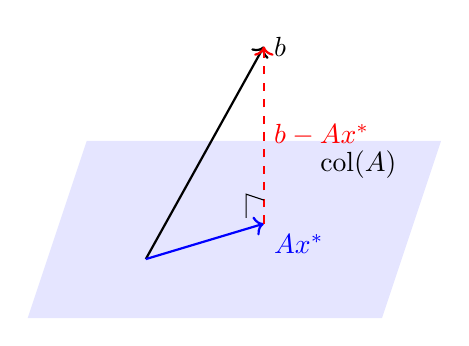
\begin{tikzpicture}[scale=1.5]
    % 列空间（平面）
    \fill[blue!10] (-1,-0.5) -- (2,-0.5) -- (2.5,1) -- (-0.5,1) -- cycle;
    \node at (1.8, 0.8) {$\text{col}(A)$};
    
    % 向量b
    \draw[->, thick] (0,0) -- (1, 1.8) node[right] {$b$};
    
    % 投影点Ax*
    \draw[->, thick, blue] (0,0) -- (1, 0.3) node[below right] {$Ax^*$};
    
    % 残差
    \draw[->, thick, red, dashed] (1, 0.3) -- (1, 1.8) node[midway, right] {$b - Ax^*$};
    
    % 直角标记
    \draw (1, 0.5) -- (0.85, 0.55) -- (0.85, 0.35);
\end{tikzpicture}
\end{center}

Sketch矩阵$S$的作用是把所有向量从$\mathbb{R}^n$映射到$\mathbb{R}^k$：
\begin{itemize}
    \item $b \mapsto Sb$
    \item $Ax \mapsto SAx$（对所有$x$）
    \item 列空间$\text{col}(A) \mapsto \text{col}(SA)$
\end{itemize}

如果$S$能\textbf{近似保持}列空间中所有向量的长度和夹角，那么压缩后的最近点问题的解应该接近原问题的解。


%==============================================================================
\subsection{子空间嵌入：理论保证}

\subsubsection{什么是子空间嵌入？}

\begin{definition}[子空间嵌入]
设$V \subset \mathbb{R}^n$是一个$d$维子空间，$\epsilon \in (0, 1)$。矩阵$S \in \mathbb{R}^{k \times n}$称为$V$的$(1 \pm \epsilon)$\textbf{子空间嵌入}，如果对所有$y \in V$：
\[
(1 - \epsilon)\|y\|^2 \leq \|Sy\|^2 \leq (1 + \epsilon)\|y\|^2
\]
\end{definition}

\textbf{理解}：子空间嵌入保证$V$中\textbf{所有}向量的长度在映射后只有$\pm \epsilon$的相对误差。

\begin{remark}[与JL引理的区别]
\begin{itemize}
    \item JL引理：保持\textbf{有限多个点}之间的距离
    \item 子空间嵌入：保持\textbf{无限多个向量}（整个子空间）的长度
\end{itemize}
子空间嵌入是更强的条件，但对于$d$维子空间，我们可以用$d$个基向量来"代表"整个子空间。
\end{remark}

\subsubsection{为什么子空间嵌入有用？}

\begin{theorem}[Sketch-and-Solve的近似保证]
设$S$是$\text{col}([A, b])$的$(1 \pm \epsilon)$子空间嵌入（注意这里需要嵌入$A$的列空间\textbf{加上}$b$）。设$x^*$是原问题的最优解，$\tilde{x}$是压缩问题的解。则：
\[
\|A\tilde{x} - b\| \leq \frac{1 + \epsilon}{1 - \epsilon} \|Ax^* - b\| \approx (1 + 2\epsilon)\|Ax^* - b\|
\]
\end{theorem}

\textbf{理解}：如果原问题的最优残差是$r^* = \|Ax^* - b\|$，那么sketch方法得到的残差最多是$(1 + O(\epsilon))r^*$。这是\textbf{乘性误差}，不是加性误差！

\begin{example}[误差的实际意义]
设原问题的最优残差$\|Ax^* - b\| = 100$（比如均方根误差是100元）。

取$\epsilon = 0.1$，则sketch方法的残差满足：
\[
\|A\tilde{x} - b\| \leq \frac{1.1}{0.9} \times 100 \approx 122
\]

即残差最多增加22\%。如果这个精度可以接受，我们就能获得巨大的加速。
\end{example}

\subsubsection{定理的证明}

\textbf{Step 1}：建立不等式链

设$r^* = Ax^* - b$是原问题的残差向量。注意$r^* \perp \text{col}(A)$（残差与列空间正交，这是最小二乘的几何性质）。

对于任意$x$，设$r_x = Ax - b$。则：
\begin{align*}
\|r_x\|^2 &= \|Ax - Ax^* + Ax^* - b\|^2 \\
&= \|A(x - x^*) + r^*\|^2 \\
&= \|A(x - x^*)\|^2 + \|r^*\|^2 \quad \text{（因为$A(x-x^*) \in \text{col}(A) \perp r^*$）}
\end{align*}

\textbf{Step 2}：利用子空间嵌入性质

因为$A(x - x^*) \in \text{col}(A)$且$r^* = Ax^* - b$可以分解为列空间内和列空间外的分量，子空间嵌入保证：
\[
(1-\epsilon)\|A(x-x^*)\|^2 \leq \|SA(x-x^*)\|^2 \leq (1+\epsilon)\|A(x-x^*)\|^2
\]

\textbf{Step 3}：比较原问题和压缩问题

$\tilde{x}$是压缩问题$\min_x \|SAx - Sb\|$的最优解，所以对任意$x$（特别是$x^*$）：
\[
\|SA\tilde{x} - Sb\|^2 \leq \|SAx^* - Sb\|^2
\]

利用子空间嵌入性质（需要一些技术细节处理$b$不在列空间的情况），可以得到：
\[
(1-\epsilon)\|A\tilde{x} - b\|^2 - \epsilon\|r^*\|^2 \leq \|SA\tilde{x} - Sb\|^2 \leq \|SAx^* - Sb\|^2 \leq (1+\epsilon)\|r^*\|^2
\]

整理得：
\[
\|A\tilde{x} - b\|^2 \leq \frac{1 + \epsilon + \epsilon}{1 - \epsilon}\|r^*\|^2 = \frac{1 + 2\epsilon}{1 - \epsilon}\|r^*\|^2
\]

取平方根并使用$(1+2\epsilon)/(1-\epsilon) \approx 1 + 3\epsilon$（当$\epsilon$较小时），得到定理的结论。


%==============================================================================
\subsection{如何构造Sketch矩阵？}

\subsubsection{从JL引理到子空间嵌入}

\begin{theorem}[子空间嵌入的存在性]
设$V$是$\mathbb{R}^n$中的$d$维子空间，$\epsilon \in (0, 1)$。如果$S \in \mathbb{R}^{k \times n}$的每个元素独立采样自$N(0, 1/k)$，且
\[
k = O\left(\frac{d}{\epsilon^2}\right)
\]
则$S$以高概率是$V$的$(1 \pm \epsilon)$子空间嵌入。
\end{theorem}

\textbf{关键点}：$k$只依赖于子空间维度$d$和精度$\epsilon$，\textbf{不依赖于}原始维度$n$！

\begin{example}[所需的sketch维度]
\begin{center}
\begin{tabular}{cccc}
\toprule
原始维度$n$ & 特征数$d$ & 精度$\epsilon$ & sketch维度$k$ \\
\midrule
$10^8$ & 1000 & 0.1 & $\approx 100000$ \\
$10^8$ & 1000 & 0.5 & $\approx 4000$ \\
$10^8$ & 100 & 0.1 & $\approx 10000$ \\
$10^6$ & 1000 & 0.1 & $\approx 100000$ \\
\bottomrule
\end{tabular}
\end{center}

观察：$k$与$n$完全无关！当$n$从$10^6$变到$10^8$（增加100倍），$k$不变。
\end{example}

\subsubsection{证明思路：覆盖网}

为什么保持$d$维子空间只需要$O(d/\epsilon^2)$维？

\textbf{核心想法}：用有限个点"覆盖"无限的子空间。

\begin{definition}[$\delta$-网]
集合$\mathcal{N}$称为单位球$S^{d-1}$的$\delta$-网，如果对任意$v \in S^{d-1}$，存在$u \in \mathcal{N}$使得$\|v - u\| \leq \delta$。
\end{definition}

\begin{lemma}[网的大小]
$d$维单位球存在大小为$(1 + 2/\delta)^d$的$\delta$-网。
\end{lemma}

\begin{example}[网的大小计算]
设$d = 100$，$\delta = 0.5$。网的大小$\leq (1 + 4)^{100} = 5^{100} \approx 10^{70}$。

虽然这个数字很大，但它是$d$的指数，而不是$n$的函数！
\end{example}

\textbf{证明思路}：
\begin{enumerate}
    \item 构造$V$中单位球的$\delta$-网$\mathcal{N}$，大小$|\mathcal{N}| \leq (3/\delta)^d$
    \item 用JL引理保证$\mathcal{N}$中所有点的长度被保持：需要$k = O(\log|\mathcal{N}|/\epsilon^2) = O(d\log(1/\delta)/\epsilon^2)$
    \item 用三角不等式从网点推广到整个子空间：如果网点的长度保持误差$\epsilon/2$，则整个子空间的误差$\leq \epsilon$
\end{enumerate}

\subsubsection{各种Sketch矩阵}

实际中有多种选择，各有优缺点：

\textbf{1. 高斯sketch}
\[
S_{ij} \sim N(0, 1/k) \text{ 独立}
\]
\begin{itemize}
    \item 优点：理论分析简单，误差界最优
    \item 缺点：计算$SA$需要$O(nkd)$时间，矩阵$S$本身需要$O(nk)$存储
\end{itemize}

\textbf{2. 稀疏嵌入（CountSketch）}
\[
S_{ij} = \begin{cases}
+1/\sqrt{s} & \text{以概率 } s/(2n) \\
-1/\sqrt{s} & \text{以概率 } s/(2n) \\
0 & \text{以概率 } 1 - s/n
\end{cases}
\]
每列恰好有$s$个非零元素。
\begin{itemize}
    \item 优点：计算$SA$只需$O(\text{nnz}(A))$时间（$\text{nnz}$=非零元素个数）
    \item 缺点：需要略大的$k$来达到同样精度
\end{itemize}


\begin{example}[CountSketch 计算过程示例]
    假设我们将 $d=4$ 维向量投影到 $k=2$ 维，设置稀疏度 $s=1$（每列仅有一个非零值 $\pm 1$）。
    
    对于输入向量 $x = [x_1, x_2, x_3, x_4]^\top = [10, 20, 30, 40]^\top$：
    \[
    \underbrace{\begin{bmatrix}
    y_1 \\ y_2
    \end{bmatrix}}_{y = Sx}
    =
    \underbrace{\begin{bmatrix}
    1/\sqrt{2} & 0 & -1/\sqrt{2}  & 0 \\
    0 & -1/\sqrt{2}  & 0 & 1/\sqrt{2} 
    \end{bmatrix}}_{S \in \{0, \pm 1\}^{2 \times 4}}
    \begin{bmatrix}
    10 \\ 20 \\ 30 \\ 40
    \end{bmatrix}
    \]
    
    \textbf{计算逻辑（哈希与符号翻转）}：
    \begin{itemize}
        \item \textbf{第1行}（桶1）：收集了 $x_1$ 和 $x_3$（符号分别为 $+,-$）。\\
        $\Rightarrow y_1 = 1 \cdot 10 + (-1) \cdot 30 = -20$
        \item \textbf{第2行}（桶2）：收集了 $x_2$ 和 $x_4$（符号分别为 $-,+$）。\\
        $\Rightarrow y_2 = (-1) \cdot 20 + 1 \cdot 40 = 20$
    \end{itemize}
    
    \textbf{观察}：实际上并没有进行真正的矩阵乘法，只是将输入元素$x_i$以随机符号$\sigma_i$“扔”进随机的桶$h(i)$中。
\end{example}


\subsubsection*{直观理解：为什么稀疏投影需要更大的 $k$？}

虽然稀疏投影（Sparse Embedding）极大地加速了矩阵乘法，但它在“信息混合”的效率上不如稠密高斯矩阵，因此通常需要略大的目标维度 $k$ 来补偿精度的损失。

\begin{enumerate}
    \item \textbf{稠密矩阵（全员参与，混合均匀）}：
    在高斯随机投影中，输出向量的每一个分量 $y_i$ 都是输入向量 $x$ 所有 $d$ 个维度的线性组合。
    \[ y_i = \sum_{j=1}^d G_{ij} x_j \]
    根据\textbf{中心极限定理（CLT）}，即使 $d$ 不大，误差也能迅速互相抵消，使得 $\|y\|^2$ 非常紧密地集中在 $\|x\|^2$ 周围。因此，$k$ 仅需满足 $O(\epsilon^{-2} \log n)$ 即可。

    \item \textbf{稀疏矩阵（抽样参与，混合不足）}：
    在 CountSketch 中，每个输入维度 $x_j$ 仅对极少数（如 $s$ 个）输出维度有贡献。
    \begin{itemize}
        \item \textbf{最坏情况（稀疏向量风险）}：如果输入向量 $x$ 本身非常稀疏（例如 $x=(100, 1, 0, \dots, 0)$），其模长主要由那个 $100$ 决定。
        \item 在稀疏投影下，这个 $100$ 仅被“扔”进了极少数桶里。如果这几个桶的随机符号没有很好地平衡，或者发生了剧烈的哈希碰撞（Collision），估计的方差就会显著增大。
    \end{itemize}
    
    \item \textbf{时空权衡（Time-Space Trade-off）}：
    为了弥补这种由于“混合不均匀”带来的高方差，我们需要更多的桶（即更大的 $k$）来保证在大数定律的作用下误差收敛。
    \[
    \text{CountSketch 复杂度：} \quad \underbrace{O(\text{nnz}(A))}_{\text{极快的时间}} \quad \text{vs} \quad \underbrace{k_{\text{sparse}} > k_{\text{dense}}}_{\text{稍大的空间}}
    \]
\end{enumerate}


\textbf{3. 子采样随机化Hadamard变换（SRHT）}
\[
S = \sqrt{\frac{n}{k}} P H D
\]
其中$D$是随机$\pm 1$对角矩阵，$H$是Hadamard矩阵，$P$是随机选取$k$行的采样矩阵。
\begin{itemize}
    \item 优点：计算$SA$只需$O(nd\log k)$时间（利用快速Hadamard变换）
    \item 缺点：实现较复杂
\end{itemize}

\begin{center}
\begin{tabular}{lccc}
\toprule
Sketch类型 & 计算$SA$的时间 & 所需$k$ & 存储$S$ \\
\midrule
高斯 & $O(nkd)$ & $O(d/\epsilon^2)$ & $O(nk)$ \\
稀疏(CountSketch) & $O(\text{nnz}(A))$ & $O(d^2/\epsilon^2)$ & $O(n)$ \\
SRHT & $O(nd\log k)$ & $O(d/\epsilon^2)$ & $O(n)$ \\
\bottomrule
\end{tabular}
\end{center}

\begin{example}[SRHT 的“能量摊平”效应]
    设输入维度 $n=4$，降维目标 $k=2$。
    
    \textbf{1. 为什么要预处理 $D$？}
    假设输入向量是全 1 向量 $x = [1, 1, 1, 1]^\top$（能量分布非常均匀）。
    如果不乘 $D$，直接做 Hadamard 变换：
    \[
    H x = \begin{bmatrix}
    1 & 1 & 1 & 1 \\
    1 & -1 & 1 & -1 \\
    1 & 1 & -1 & -1 \\
    1 & -1 & -1 & 1
    \end{bmatrix}
    \begin{bmatrix}
    1 \\ 1 \\ 1 \\ 1
    \end{bmatrix}
    =
    \begin{bmatrix}
    4 \\ 0 \\ 0 \\ 0
    \end{bmatrix}
    \]
    \textbf{灾难}：能量全部集中在第一个分量！如果随机采样 $P$ 恰好没选中第一行，投影后的模长就是 0，误差无穷大。

    \textbf{2. 加入随机符号 $D$ 后的流程}：
    设随机对角矩阵 $D = \text{diag}(1, -1, 1, 1)$。
    \begin{itemize}
        \item \textbf{Step 1: 随机翻转（Preconditioning）} \\
        $z = Dx = [1, -1, 1, 1]^\top$。向量看起来变得“杂乱”了。
        
        \item \textbf{Step 2: Hadamard 混合（Mixing）} \\
        利用快速变换计算 $w = Hz$：
        \[
        w = H \begin{bmatrix} 1 \\ -1 \\ 1 \\ 1 \end{bmatrix} = \begin{bmatrix} 2 \\ 2 \\ 2 \\ -2 \end{bmatrix}
        \]
        \textbf{关键观察}：能量从原来的“集中状态”变成了完美的“均匀分布”（每个分量绝对值都是2）。
        
        \item \textbf{Step 3: 随机采样（Sampling）} \\
        无论 $P$ 选取哪两行（比如第2和4行），都能捕获到成比例的能量，不会出现“漏网之鱼”。最后乘上系数 $\sqrt{n/k}$ 恢复模长即可。
    \end{itemize}
\end{example}



\subsubsection*{补充背景：Hadamard 变换与快速算法}

\textbf{1. 什么是 Hadamard 矩阵？}
Hadamard 矩阵 $H_n$ 是一个 $n \times n$ 的正交矩阵（$n$ 通常为 2 的幂），其元素仅包含 $+1$ 和 $-1$。它通过 \textbf{Sylvester 递归构造法} 定义：

\[
H_1 = [1], \quad
H_{2n} = \begin{bmatrix}
H_n & H_n \\
H_n & -H_n
\end{bmatrix}
\]

例如 $n=2$ 和 $n=4$ 时：
\[
H_2 = \begin{bmatrix} 1 & 1 \\ 1 & -1 \end{bmatrix}, \quad
H_4 = \begin{bmatrix}
1 & 1 & 1 & 1 \\
1 & -1 & 1 & -1 \\
1 & 1 & -1 & -1 \\
1 & -1 & -1 & 1
\end{bmatrix}
\]
它就像一个只由方波（Square Waves）构成的傅里叶变换基底。

\textbf{2. 为什么它快？（Fast Walsh-Hadamard Transform, FWHT）}
直接计算 $y = H_n x$ 需要做矩阵乘法，复杂度为 $O(n^2)$。
利用其递归结构，我们可以像 FFT（快速傅里叶变换）一样使用分治法加速：

把向量 $x$ 分为上半部分 $x_L$ 和下半部分 $x_R$：
\[
H_{2n} x = \begin{bmatrix} H_n & H_n \\ H_n & -H_n \end{bmatrix} \begin{bmatrix} x_L \\ x_R \end{bmatrix}
= \begin{bmatrix} H_n (x_L + x_R) \\ H_n (x_L - x_R) \end{bmatrix}
\]

\textbf{复杂度分析}：
设 $T(n)$ 为计算 $H_n x$ 所需的操作次数。
\[
T(n) = \underbrace{2 T(n/2)}_{\text{两个子问题}} + \underbrace{O(n)}_{\text{向量加减法}}
\]
根据主定理（Master Theorem），$T(n) = O(n \log n)$。

\textbf{核心优势}：
\begin{itemize}
    \item \textbf{速度}：从 $O(n^2)$ 降到 $O(n \log n)$。对于 $n=1024$，速度提升约 100 倍。
    \item \textbf{无乘法}：整个过程只涉及\textbf{加法和减法}（因为元素是 $\pm 1$），这在硬件实现上比需要浮点乘法的 FFT 还要快。
\end{itemize}

\subsubsection*{直观理解：为什么 SRHT 有效？}

SRHT 利用了 \textbf{不确定性原理（Uncertainty Principle）}：在频域和时域中，信号不可能同时是稀疏的。

\begin{enumerate}
    \item \textbf{Hadamard 变换的作用}：类似于傅里叶变换，Hadamard 矩阵 $H$ 是一个稠密的混合器。它能将“稀疏”的向量（如标准基）转换为“稠密”的向量（所有分量都不为0）。
    
    \item \textbf{随机对角阵 $D$ 的必要性}：
    虽然 $H$ 能把稀疏变稠密，但它也能把稠密变稀疏（如 Example 中所示，$H$ 把全1向量变成冲击向量）。
    \textbf{$D$ 的作用是“平滑化”}：它随机打乱输入信号的相位，确保 $Dx$ 不会落在 $H$ 的“盲区”里。这保证了 $HDx$ 的能量均匀分布在所有坐标上。
    
    \item \textbf{采样的安全性}：
    一旦能量被 $H$ 均匀摊平，随机采样 $P$ 就变得非常安全且准确（类似于从搅拌均匀的咖啡中舀一勺，浓度一定代表整体）。
\end{enumerate}

\subsubsection*{关于表格的补充说明}
\begin{itemize}
    \item \textbf{最好的平衡}：SRHT 结合了 Gaussian 的低维度需求（$k \approx O(d)$）和 CountSketch 的快速计算特性（利用 FFT/FWHT 结构）。
    \item \textbf{表格中的 $k$}：注意表格中 CountSketch 的 $k$ 依赖于 $O(d^2)$ 或 $O(k^2)$（取决于具体分析），而 SRHT 的 $k$ 几乎与 Gaussian 一样优秀，通常仅多一个 $\log d$ 因子：$k \sim O(\epsilon^{-2} \log d)$。这使得 SRHT 在高精度要求下比 CountSketch 更具优势。
\end{itemize}
%==============================================================================
\subsection{复杂度分析}

\subsubsection{总体复杂度}

设我们使用SRHT作为sketch矩阵，$k = O(d/\epsilon^2)$。

\textbf{精确求解}：$O(nd^2)$

\textbf{Sketch-and-Solve}：
\begin{enumerate}
    \item 计算$SA$：$O(nd\log k)$
    \item 计算$Sb$：$O(n\log k)$
    \item 求解压缩问题：$O(kd^2) = O(d^3/\epsilon^2)$
    \item 总计：$O(nd\log(d/\epsilon) + d^3/\epsilon^2)$
\end{enumerate}

\begin{example}[加速比计算]
设$n = 10^8$，$d = 1000$，$\epsilon = 0.1$。

\textbf{精确求解}：$O(nd^2) = O(10^8 \times 10^6) = O(10^{14})$

\textbf{Sketch-and-Solve}：
\begin{itemize}
    \item $k = O(d/\epsilon^2) = O(10^5)$
    \item 计算$SA$：$O(nd\log k) = O(10^8 \times 1000 \times 17) \approx O(1.7 \times 10^{12})$
    \item 求解压缩问题：$O(kd^2) = O(10^5 \times 10^6) = O(10^{11})$
    \item 总计：$O(1.7 \times 10^{12})$
\end{itemize}

加速比：$\frac{10^{14}}{1.7 \times 10^{12}} \approx 60$倍！

代价：残差增加最多$(1+O(\epsilon)) = 1.3$倍。
\end{example}

\subsubsection{何时Sketch方法更优？}

Sketch-and-Solve的优势在$n \gg d$时最明显。

\textbf{临界点分析}：当$nd\log k < nd^2$，即$\log k < d$时，sketch方法更快。

因为$k = O(d/\epsilon^2)$，所以$\log k = O(\log d)$，这个条件几乎总是满足的。

\textbf{真正的收益}：把$O(nd^2)$中对$n$的线性依赖变成了$O(nd\log k)$，从$d^2$变成了$d\log k$。

\begin{example}[不同$n/d$比例的比较]
固定$d = 1000$，$\epsilon = 0.1$：

\begin{center}
\begin{tabular}{ccccc}
\toprule
$n$ & $n/d$ & 精确方法 & Sketch方法 & 加速比 \\
\midrule
$10^4$ & 10 & $10^{10}$ & $10^{9}$ & 10x \\
$10^6$ & $10^3$ & $10^{12}$ & $2\times10^{10}$ & 50x \\
$10^8$ & $10^5$ & $10^{14}$ & $2\times10^{12}$ & 50x \\
$10^{10}$ & $10^7$ & $10^{16}$ & $2\times10^{14}$ & 50x \\
\bottomrule
\end{tabular}
\end{center}

当$n/d$超过某个阈值后，加速比趋于稳定（约$d/\log k$倍）。
\end{example}


%==============================================================================
\subsection{实际应用与扩展}

\subsubsection{应用场景}

\textbf{1. 大规模线性回归}
\begin{itemize}
    \item 互联网广告点击率预测：数十亿样本，数千特征
    \item 推荐系统中的矩阵分解
\end{itemize}

\textbf{2. 核岭回归的近似}
\begin{itemize}
    \item 原问题需要$O(n^3)$时间
    \item 用随机特征+sketch可以降到近乎线性时间
\end{itemize}

\textbf{3. 流式/在线学习}
\begin{itemize}
    \item 数据以流的形式到达
    \item 维护sketch $SA$和$Sb$，可以增量更新
    \item 空间只需$O(kd)$而不是$O(nd)$
\end{itemize}

\subsubsection{迭代精化}

Sketch-and-Solve得到的是近似解。如果需要更高精度，可以用迭代方法精化：

\textbf{Sketch-and-Precondition}：
\begin{enumerate}
    \item 用sketch方法计算$R = $ Cholesky$(SA)^T(SA)$
    \item 用$R$作为预条件子，运行迭代方法（如LSQR）
    \item 预条件子大幅加速收敛
\end{enumerate}

这种方法可以达到机器精度，同时保持sketch方法的计算优势。

\subsubsection{与其他方法的比较}

\begin{center}
\begin{tabular}{lccc}
\toprule
方法 & 时间复杂度 & 精度 & 适用场景 \\
\midrule
精确QR & $O(nd^2)$ & 精确 & 小规模 \\
随机梯度下降 & $O(nd/\epsilon)$ & $\epsilon$-近似 & 在线学习 \\
Sketch-and-Solve & $O(nd\log k + d^3/\epsilon^2)$ & $(1+\epsilon)$-近似 & 大规模批处理 \\
Sketch + 迭代 & $O(nd\log k + d^3\log(1/\epsilon))$ & $\epsilon$-精确 & 需要高精度 \\
\bottomrule
\end{tabular}
\end{center}

\begin{remark}[如何选择？]
\begin{itemize}
    \item 如果$n$不太大（$n < 10^5$），直接用精确方法
    \item 如果只需要粗略近似且数据在线到达，用SGD
    \item 如果$n$很大、需要$(1+\epsilon)$近似、数据可以批处理，用Sketch-and-Solve
    \item 如果需要高精度，用Sketch作为预条件子加速迭代方法
\end{itemize}
\end{remark}


\subsubsection*{评论：Sketching 回归与经典渐近理论的本质区别}

尽管 Sketching 方法（如 CountSketch、SRHT）和经典统计渐近理论（Asymptotic Theory）都涉及“大样本”和“近似”，但它们的哲学出发点和数学保证截然不同。

\begin{enumerate}
    \item \textbf{随机性的来源（Algorithmic vs. Statistical Randomness）}
    \begin{itemize}
        \item \textbf{经典理论}：假设算法是确定的（如最小二乘法 OLS），误差来源于\textbf{数据的生成过程}（即噪声 $\epsilon$）。关注的是当 $n \to \infty$ 时，估计量 $\hat{\beta}$ 是否收敛到真实参数 $\beta_{true}$（一致性）。
        \item \textbf{Sketching}：假设数据 $X, y$ 是固定的（Fixed Design），误差来源于\textbf{算法内部的随机投影} $S$。我们不关心数据的分布，而是关心“无论数据多么糟糕，随机投影以高概率（w.h.p.）给出一个好解”。
    \end{itemize}

    \item \textbf{近似的目标（Loss vs. Parameters）}
    \begin{itemize}
        \item \textbf{经典理论}：追求参数估计的\textbf{效率（Efficiency）}，即在无偏估计中方差最小（BLUE 性质）。
        \item \textbf{Sketching}：通常追求\textbf{目标函数的近似（Cost Approximation）}。RandNLA 的典型保证形式为：
        \[
        \|X \tilde{\beta} - y\|^2 \leq (1+\epsilon) \min_{\beta} \|X\beta - y\|^2
        \]
        即它保证能找到一个“预测效果几乎一样好”的解，但不一定保证 $\tilde{\beta}$ 在欧氏距离上非常接近 $\hat{\beta}_{OLS}$（除非矩阵具有强凸性/条件数很好）。
    \end{itemize}

    \item \textbf{偏差与方差的权衡}
    \begin{itemize}
        \item 使用 Sketching 求出的解 $\tilde{\beta} = (X^T S^T S X)^{-1} X^T S^T S y$ 往往是原始 OLS 解的一个\textbf{有偏估计}（或者是方差膨胀后的估计）。
        \item Sketching 可以被视为一种\textbf{计算换精度的交易}：我们主动引入了额外的“算法噪声”（通过降低维度 $k \ll n$），以换取从 $O(nd^2)$ 到 $O(\text{nnz}(A) + d^3)$ 的计算加速。只要 $k$ 足够大，这种算法噪声通常远小于原始数据的统计噪声。
    \end{itemize}
\end{enumerate}

\textbf{一句话总结}：经典理论问的是“我有多少数据才能接近真理？”，而 Sketching 问的是“我可以扔掉多少数据，却依然不偏离最优解太多？”。


\section{理论对比：经典统计推断 vs. 随机数值线性代数 (RandNLA)}

\textbf{符号约定}：在此对比中，我们考虑线性回归问题 $y = X\beta + \epsilon$。
\begin{itemize}
    \item $n$：样本量（$X$ 的行数，通常极大）。
    \item $d$：特征维度（$X$ 的列数，即未知参数 $\beta$ 的维度）。
    \item $k$：Sketching 后的样本量（降维后的行数）。
\end{itemize}

我们通过回答同一个问题来对比这两套理论：“为了保证得到一个好的解 $\beta$，我们需要多少样本？”

\subsection{1. 经典统计学习理论 (Classical Statistical Learning)}
\textbf{背景假设}：数据矩阵 $X \in \mathbb{R}^{n \times d}$ 的每一行 $(x_i, y_i)$ 都是\textbf{随机生成}的，独立同分布 (i.i.d.) 采样自某个分布。

\begin{itemize}
    \item \textbf{关注点}：\textbf{泛化误差 (Generalization Error)}。
    即：在 $n$ 个样本上训练出的 $\hat{\beta}$，能否在新的测试数据上表现良好？
    
    \item \textbf{样本量要求 ($n$ vs $d$)}：
    根据统计学习理论（如 VC 维），为了防止过拟合并不以概率 $1-\delta$ 保证误差界限，真实样本量 $n$ 必须显著大于特征维度 $d$。通常要求：
    \[
    n \gtrsim O\left(\frac{d + \log(1/\delta)}{\epsilon^2}\right)
    \]
    
    \item \textbf{直觉 (大数定律)}：
    这里的 $n$ 是对抗噪声的武器。我们需要足够多的 $n$ 来“平均”掉噪声 $\epsilon$，从而让真实的信号结构（维度为 $d$）浮现出来。
\end{itemize}

\subsection{2. 随机投影/Sketching 理论 (RandNLA)}
\textbf{背景假设}：数据矩阵 $X \in \mathbb{R}^{n \times d}$ 是\textbf{固定}的 (Fixed Design)，即便是最坏情况（Worst-case）的数据。随机性仅来源于算法生成的投影矩阵 $S \in \mathbb{R}^{k \times n}$。

\begin{itemize}
    \item \textbf{关注点}：\textbf{算法逼近误差 (Algorithmic Approximation)}。
    即：我们不解原始的 $n$ 行方程组，而是解压缩后的 $k$ 行方程组 $\min \|S(X\beta - y)\|^2$。求出的解 $\tilde{\beta}$ 能否接近原始最优解？
    
    \item \textbf{Sketch 维度要求 ($k$ vs $d$)}：
    为了保证解的相对误差在 $(1+\epsilon)$ 范围内，压缩后的行数 $k$ 并不依赖于原始样本量 $n$，而只依赖于特征维度 $d$。通常只需：
    \[
    k \gtrsim O\left(\frac{d \log d}{\epsilon^2}\right) \quad (\text{SRHT 或 Leverage Score})
    \]
    \textbf{关键点}：即使原始数据 $n = 100$ 亿，只要特征 $d=50$，我们只需要保留 $k \approx 2000$ 行左右的数据即可求解，与 $n$ 无关。
    
    \item \textbf{直觉 (子空间嵌入)}：
    这是利用高维几何的性质。$X$ 的列空间构成了一个 $d$ 维子空间。Sketching 矩阵 $S$ 的作用是把这个子空间“保距”地嵌入到低维空间中。只要 $k$ 足够容纳 $d$ 维信息，解就是准的。
\end{itemize}

\subsection{3. 深入：高维概率论的“反直觉”特点}
Sketching 之所以有效，是因为高维空间具有一些与二维/三维直觉截然不同的性质。

\subsubsection{A. 测度集中现象 (Concentration of Measure)}
在低维空间，质量分布在整个球体内部。但在高维空间 ($d \to \infty$)，\textbf{几乎所有的质量都集中在球壳表面，甚至集中在赤道附近的一条窄带上}。

对于高维单位球体上的 Lipschitz 函数 $f$，其值偏离均值的概率呈指数级下降：
\[
\mathbb{P}(|f(x) - \mathbb{E}[f]| \geq t) \leq 2 \exp(-C d t^2)
\]
\textbf{意义}：当我们把向量投影到随机子空间时，它的模长不仅仅是“平均”等于原模长，而是\textbf{以极大概率非常精确地等于}原模长。在高维空间，“随机”意味着“确定”。

\subsubsection{B. 准正交性 (Quasi-Orthogonality)}
在低维空间，两个随机向量很少垂直。但在高维空间，\textbf{任意两个独立的随机向量，以极大概率几乎是垂直的}。

\textbf{意义}：随机投影矩阵 $S$ 的每一行都捕捉了原始空间的一个独立“切面”，行与行之间几乎没有冗余信息。

\subsubsection{C. 维度诅咒 vs. 维度祝福}
\begin{itemize}
    \item \textbf{诅咒 (Curse)}：在经典优化中，$d$ 越大，搜索空间呈指数爆炸，需要更多的 $n$ 来填满空间。
    \item \textbf{祝福 (Blessing)}：在高维概率论中，$d$ 越大，随机变量的方差越小，统计规律越稳定。Sketching正是利用这种“高维祝福”来实现降维。
\end{itemize}

\subsection{4. 总结对比表}

\begin{center}
\begin{tabular}{lcc}
\toprule
\textbf{特性} & \textbf{经典统计推断 (IID)} & \textbf{高维 Sketching 理论} \\
\midrule
\textbf{核心工具} & 大数定律, 中心极限定理 & 测度集中, JL 引理 \\
\textbf{数据假设} & 随机生成 (IID) & 任意固定 (Worst-case) \\
\textbf{随机性来源} & 数据本身 (噪声) & 算法引入 (投影矩阵 $S$) \\
\textbf{追求目标} & 参数收敛 ($\hat{\beta} \to \beta^*$) & 目标函数近似 (Cost Preservation) \\
\textbf{样本/维度关系} & $n \gg d$ (越多越好) & $k \gtrsim d \log d$ (与 $n$ 无关) \\
\textbf{高维视角} & 维度是负担 (Curse) & 维度带来稳定性 (Blessing) \\
\bottomrule
\end{tabular}
\end{center}


\section{随机矩阵乘法：用采样加速计算}

\subsection{问题的提出（0:25--0:30）}

\subsubsection{矩阵乘法的计算瓶颈}

矩阵乘法是科学计算中最基础也最耗时的操作之一。给定$A \in \mathbb{R}^{m \times n}$和$B \in \mathbb{R}^{n \times p}$，计算乘积$AB$的标准算法需要$O(mnp)$次运算。

\begin{example}[具体规模感受]
在推荐系统中，我们经常需要计算用户-商品评分矩阵的低秩分解。假设：
\begin{itemize}
    \item 用户矩阵$A \in \mathbb{R}^{10^6 \times 10^4}$（100万用户，1万维隐因子）
    \item 商品矩阵$B \in \mathbb{R}^{10^4 \times 10^5}$（1万维隐因子，10万商品）
    \item 计算$AB$需要$10^6 \times 10^4 \times 10^5 = 10^{15}$次运算
    \item 即使每秒$10^{12}$次运算（1 TFLOP），也需要1000秒$\approx$17分钟
\end{itemize}
如果只需要一个近似结果，能否大幅加速？
\end{example}

\subsubsection{矩阵乘法的外积视角}

理解随机化方法的关键是换一个视角看矩阵乘法。

\textbf{传统视角（内积）}：$(AB)_{ij} = \sum_{k=1}^n A_{ik} B_{kj}$，即$A$的第$i$行与$B$的第$j$列的内积。

\textbf{外积视角}：把$AB$写成$n$个秩1矩阵的和：
\[
AB = \sum_{i=1}^n A_{\cdot i} B_{i \cdot}
\]
其中$A_{\cdot i} \in \mathbb{R}^{m \times 1}$是$A$的第$i$列，$B_{i \cdot} \in \mathbb{R}^{1 \times p}$是$B$的第$i$行。

\begin{example}[外积分解的具体例子]
设
\[
A = \begin{pmatrix} 1 & 2 \\ 3 & 4 \end{pmatrix}, \quad B = \begin{pmatrix} 5 & 6 \\ 7 & 8 \end{pmatrix}
\]

传统计算：
\[
AB = \begin{pmatrix} 1\times5 + 2\times7 & 1\times6 + 2\times8 \\ 3\times5 + 4\times7 & 3\times6 + 4\times8 \end{pmatrix} = \begin{pmatrix} 19 & 22 \\ 43 & 50 \end{pmatrix}
\]

外积视角：
\begin{align*}
AB &= \underbrace{\begin{pmatrix} 1 \\ 3 \end{pmatrix} \begin{pmatrix} 5 & 6 \end{pmatrix}}_{\text{第1列} \times \text{第1行}} + \underbrace{\begin{pmatrix} 2 \\ 4 \end{pmatrix} \begin{pmatrix} 7 & 8 \end{pmatrix}}_{\text{第2列} \times \text{第2行}} \\
&= \begin{pmatrix} 5 & 6 \\ 15 & 18 \end{pmatrix} + \begin{pmatrix} 14 & 16 \\ 28 & 32 \end{pmatrix} = \begin{pmatrix} 19 & 22 \\ 43 & 50 \end{pmatrix}
\end{align*}
\end{example}

\textbf{随机化的核心思想}：既然$AB$是$n$项的和，我们能否只随机采样$k$项（$k \ll n$），用这$k$项来近似整个和？这就像用民意调查（采样1000人）来估计全国的投票意向（上亿人）。


%==============================================================================
\subsection{随机采样算法（0:30--0:35）}

\subsubsection{算法描述}

\textbf{输入}：矩阵$A \in \mathbb{R}^{m \times n}$，$B \in \mathbb{R}^{n \times p}$，采样次数$k$

\textbf{算法}：
\begin{enumerate}
    \item \textbf{选择采样概率}：确定概率分布$p_1, \ldots, p_n$，满足$\sum_{i=1}^n p_i = 1$，$p_i > 0$
    \item \textbf{独立采样$k$次}：每次以概率$p_i$选中索引$i$
    \item \textbf{构造缩放后的列和行}：设第$t$次采样选中了索引$i_t$，构造
    \[
    C_t = \frac{1}{\sqrt{k p_{i_t}}} A_{\cdot i_t}, \quad R_t = \frac{1}{\sqrt{k p_{i_t}}} B_{i_t \cdot}
    \]
    \item \textbf{输出}：$\widetilde{AB} = CR = \sum_{t=1}^k C_t R_t$
\end{enumerate}

\textbf{输出形式}：实际上我们构造了两个矩阵$C \in \mathbb{R}^{m \times k}$和$R \in \mathbb{R}^{k \times p}$，输出$CR$。

\subsubsection{为什么需要缩放因子$\frac{1}{\sqrt{kp_i}}$？}

这个看起来奇怪的缩放因子是为了保证\textbf{无偏性}——即估计量的期望等于真实值。

\begin{example}[不缩放会怎样？]
考虑最简单的情况：$n=2$，均匀采样（$p_1 = p_2 = 1/2$），采样$k=1$次。

如果不缩放，我们的估计是：
\[
\widetilde{AB} = \begin{cases}
A_{\cdot 1} B_{1 \cdot} & \text{概率 } 1/2 \\
A_{\cdot 2} B_{2 \cdot} & \text{概率 } 1/2
\end{cases}
\]

期望是：
\[
\mathbb{E}[\widetilde{AB}] = \frac{1}{2} A_{\cdot 1} B_{1 \cdot} + \frac{1}{2} A_{\cdot 2} B_{2 \cdot} = \frac{1}{2} AB
\]

这只有真实值的一半！我们\textbf{低估}了。
\end{example}

\subsubsection{无偏性的严格验证}

设第$t$次采样选中索引$i_t$，则单次采样的贡献是：
\[
C_t R_t = \frac{1}{k p_{i_t}} A_{\cdot i_t} B_{i_t \cdot}
\]

计算期望：
\begin{align*}
\mathbb{E}[C_t R_t] &= \sum_{i=1}^n P(i_t = i) \cdot \frac{1}{k p_i} A_{\cdot i} B_{i \cdot} \\
&= \sum_{i=1}^n p_i \cdot \frac{1}{k p_i} A_{\cdot i} B_{i \cdot} \quad \text{（因为$P(i_t = i) = p_i$）}\\
&= \frac{1}{k} \sum_{i=1}^n A_{\cdot i} B_{i \cdot} \\
&= \frac{1}{k} AB
\end{align*}

因为$k$次采样独立，所以：
\[
\mathbb{E}[CR] = \mathbb{E}\left[\sum_{t=1}^k C_t R_t\right] = \sum_{t=1}^k \mathbb{E}[C_t R_t] = k \cdot \frac{1}{k} AB = AB
\]

\textbf{结论}：无论选择什么采样概率$p_i$（只要都是正的），估计量都是无偏的！

\begin{example}[完整的数值例子]
继续用之前的例子：
\[
A = \begin{pmatrix} 1 & 2 \\ 3 & 4 \end{pmatrix}, \quad B = \begin{pmatrix} 5 & 6 \\ 7 & 8 \end{pmatrix}, \quad AB = \begin{pmatrix} 19 & 22 \\ 43 & 50 \end{pmatrix}
\]

设$k=1$，均匀采样$p_1 = p_2 = 1/2$。

\textbf{情况1}：采样选中$i=1$
\[
\widetilde{AB} = \frac{1}{1 \times 0.5} \begin{pmatrix} 1 \\ 3 \end{pmatrix} \begin{pmatrix} 5 & 6 \end{pmatrix} = 2 \begin{pmatrix} 5 & 6 \\ 15 & 18 \end{pmatrix} = \begin{pmatrix} 10 & 12 \\ 30 & 36 \end{pmatrix}
\]

\textbf{情况2}：采样选中$i=2$
\[
\widetilde{AB} = \frac{1}{1 \times 0.5} \begin{pmatrix} 2 \\ 4 \end{pmatrix} \begin{pmatrix} 7 & 8 \end{pmatrix} = 2 \begin{pmatrix} 14 & 16 \\ 28 & 32 \end{pmatrix} = \begin{pmatrix} 28 & 32 \\ 56 & 64 \end{pmatrix}
\]

\textbf{验证无偏性}：
\[
\mathbb{E}[\widetilde{AB}] = \frac{1}{2} \begin{pmatrix} 10 & 12 \\ 30 & 36 \end{pmatrix} + \frac{1}{2} \begin{pmatrix} 28 & 32 \\ 56 & 64 \end{pmatrix} = \begin{pmatrix} 19 & 22 \\ 43 & 50 \end{pmatrix} = AB \quad \checkmark
\]

注意虽然期望正确，但单次估计的误差很大（例如情况1的$(1,1)$元素是10，真实值是19）。
\end{example}

\subsubsection{计算复杂度}

\textbf{精确计算}$AB$：$O(mnp)$

\textbf{随机采样方法}：
\begin{itemize}
    \item 采样$k$个索引：$O(k)$（如果预处理了累积概率）或$O(k \log n)$（二分查找）
    \item 构造$C$：复制$A$的$k$列并缩放，$O(mk)$
    \item 构造$R$：复制$B$的$k$行并缩放，$O(kp)$
    \item 计算$CR$：$O(mkp)$
    \item 总计：$O(mkp)$
\end{itemize}

\textbf{加速比}：$\frac{mnp}{mkp} = \frac{n}{k}$。如果$k = n/100$，则快100倍！


%==============================================================================
\subsection{误差分析（0:35--0:40）}

无偏性只说期望正确，但我们更关心：单次估计离真实值有多远？

\subsubsection{误差的度量}

我们用Frobenius范数来度量误差：
\[
\|AB - CR\|_F = \sqrt{\sum_{i,j} (AB - CR)_{ij}^2}
\]

这衡量的是"所有元素的均方误差"的总和。

\subsubsection{误差界定理}

\begin{theorem}[随机矩阵乘法的误差界]
设采样概率选择为
\[
p_i = \frac{\|A_{\cdot i}\| \cdot \|B_{i \cdot}\|}{\sum_{j=1}^n \|A_{\cdot j}\| \cdot \|B_{j \cdot}\|}
\]
（即按列范数与行范数的乘积成比例采样），则
\[
\mathbb{E}\|AB - CR\|_F^2 \leq \frac{\|A\|_F^2 \cdot \|B\|_F^2}{k}
\]
其中$\|A\|_F = \sqrt{\sum_{i,j} A_{ij}^2}$是Frobenius范数。
\end{theorem}

\begin{remark}[理解这个界]
\begin{itemize}
    \item 误差随$k$\textbf{线性下降}：$k$翻倍，期望误差平方减半，即误差减少$\sqrt{2} \approx 1.41$倍
    \item 误差与$\|A\|_F$和$\|B\|_F$成正比：矩阵元素越大，绝对误差越大（但相对误差可能不变）
    \item 这个界是\textbf{数据依赖}的：取决于$A$和$B$的范数结构
\end{itemize}
\end{remark}

\begin{example}[误差界的具体计算]
设$A, B \in \mathbb{R}^{1000 \times 1000}$，每个元素独立地从$N(0,1)$采样。

范数的期望：$\mathbb{E}[\|A\|_F^2] = 1000 \times 1000 \times 1 = 10^6$，所以$\|A\|_F \approx 1000$。

乘积的范数：$\|AB\|_F \approx 1000 \times 1000 = 10^6$（这是一个粗略估计）。

误差界：
\[
\mathbb{E}\|AB - CR\|_F^2 \leq \frac{10^6 \times 10^6}{k} = \frac{10^{12}}{k}
\]

如果我们想要相对误差$\frac{\|AB - CR\|_F}{\|AB\|_F} \leq 1\%$，需要：
\[
\frac{\sqrt{10^{12}/k}}{10^6} \leq 0.01 \implies \frac{10^6}{\sqrt{k}} \leq 10^4 \implies k \geq 10^4
\]

即采样1万次（原本需要求和100万项），就能达到1\%的相对误差。加速100倍！
\end{example}

\subsubsection{误差界的证明思路}

\textbf{核心工具}：方差分解。对于独立随机变量的和，方差等于各项方差之和。

设$X = CR - AB = \sum_{t=1}^k (C_t R_t - \frac{1}{k}AB)$。因为$\mathbb{E}[C_t R_t] = \frac{1}{k}AB$，所以每一项都是零均值的。

\[
\mathbb{E}\|X\|_F^2 = \mathbb{E}\left\|\sum_{t=1}^k \left(C_t R_t - \frac{1}{k}AB\right)\right\|_F^2
\]

因为各项独立且零均值：
\[
= \sum_{t=1}^k \mathbb{E}\left\|C_t R_t - \frac{1}{k}AB\right\|_F^2 = k \cdot \text{Var}(C_1 R_1)
\]

（这里用到了$k$次采样是独立同分布的）

关键是计算单次采样的方差$\text{Var}(C_1 R_1)$。经过计算（利用$\text{Var}(X) = \mathbb{E}[X^2] - (\mathbb{E}[X])^2$），可以证明当采样概率选择为$p_i \propto \|A_{\cdot i}\| \|B_{i\cdot}\|$时，方差达到最小，且满足定理中的界。

\subsubsection{误差界的完整证明}

我们要证明：当采样概率$p_i \propto \|A_{\cdot i}\| \|B_{i\cdot}\|$时，
\[
\mathbb{E}\|AB - CR\|_F^2 \leq \frac{\|A\|_F^2 \cdot \|B\|_F^2}{k}
\]

\textbf{Step 1：方差分解}

设$Y_t = C_t R_t - \frac{1}{k}AB$。由于$\mathbb{E}[C_t R_t] = \frac{1}{k}AB$，所以$Y_t$是零均值随机矩阵。

误差可以写成：
\[
CR - AB = \sum_{t=1}^k C_t R_t - AB = \sum_{t=1}^k \left(C_t R_t - \frac{1}{k}AB\right) = \sum_{t=1}^k Y_t
\]

对于独立零均值随机矩阵，Frobenius范数的平方满足可加性：
\[
\mathbb{E}\left\|\sum_{t=1}^k Y_t\right\|_F^2 = \sum_{t=1}^k \mathbb{E}\|Y_t\|_F^2 = k \cdot \mathbb{E}\|Y_1\|_F^2
\]

\textbf{Step 2：计算单次采样的方差}

展开$\mathbb{E}\|Y_1\|_F^2$：
\begin{align*}
\mathbb{E}\|Y_1\|_F^2 &= \mathbb{E}\left\|C_1 R_1 - \frac{1}{k}AB\right\|_F^2 \\
&= \mathbb{E}\|C_1 R_1\|_F^2 - 2\left\langle \mathbb{E}[C_1 R_1], \frac{1}{k}AB \right\rangle_F + \left\|\frac{1}{k}AB\right\|_F^2 \\
&= \mathbb{E}\|C_1 R_1\|_F^2 - 2\left\langle \frac{1}{k}AB, \frac{1}{k}AB \right\rangle_F + \frac{1}{k^2}\|AB\|_F^2 \\
&= \mathbb{E}\|C_1 R_1\|_F^2 - \frac{1}{k^2}\|AB\|_F^2
\end{align*}

现在计算$\mathbb{E}\|C_1 R_1\|_F^2$。注意$C_1 R_1 = \frac{1}{kp_{i_1}} A_{\cdot i_1} B_{i_1\cdot}$是秩1矩阵，其Frobenius范数为：
\[
\|C_1 R_1\|_F^2 = \frac{1}{k^2 p_{i_1}^2} \|A_{\cdot i_1}\|^2 \|B_{i_1\cdot}\|^2
\]

（这里用到了秩1矩阵$uv^T$的性质：$\|uv^T\|_F^2 = \|u\|^2 \|v\|^2$）

取期望：
\[
\mathbb{E}\|C_1 R_1\|_F^2 = \sum_{i=1}^n p_i \cdot \frac{\|A_{\cdot i}\|^2 \|B_{i\cdot}\|^2}{k^2 p_i^2} = \frac{1}{k^2} \sum_{i=1}^n \frac{\|A_{\cdot i}\|^2 \|B_{i\cdot}\|^2}{p_i}
\]

因此：
\[
\mathbb{E}\|CR - AB\|_F^2 = k \cdot \mathbb{E}\|Y_1\|_F^2 = \frac{1}{k}\sum_{i=1}^n \frac{\|A_{\cdot i}\|^2 \|B_{i\cdot}\|^2}{p_i} - \frac{1}{k}\|AB\|_F^2
\]

\textbf{Step 3：最优采样概率（第一次用柯西不等式）}

现在问题变成：如何选择$p_i$（满足$\sum_i p_i = 1$）使得$\sum_{i=1}^n \frac{\|A_{\cdot i}\|^2 \|B_{i\cdot}\|^2}{p_i}$最小？

记$a_i = \|A_{\cdot i}\| \|B_{i\cdot}\|$，我们要最小化$\sum_{i=1}^n \frac{a_i^2}{p_i}$。

应用\textbf{柯西-施瓦茨不等式}（向量形式：$(\sum x_i y_i)^2 \leq (\sum x_i^2)(\sum y_i^2)$）：

令$x_i = \frac{a_i}{\sqrt{p_i}}$，$y_i = \sqrt{p_i}$，则：
\[
\left(\sum_{i=1}^n a_i\right)^2 = \left(\sum_{i=1}^n x_i y_i\right)^2 \leq \left(\sum_{i=1}^n \frac{a_i^2}{p_i}\right) \cdot \left(\sum_{i=1}^n p_i\right) = \sum_{i=1}^n \frac{a_i^2}{p_i}
\]

即：
\[
\sum_{i=1}^n \frac{a_i^2}{p_i} \geq \left(\sum_{i=1}^n a_i\right)^2
\]

等号成立当且仅当$\frac{x_i}{y_i} = \text{const}$，即$\frac{a_i}{p_i} = \text{const}$，即：
\[
p_i = \frac{a_i}{\sum_j a_j} = \frac{\|A_{\cdot i}\| \|B_{i\cdot}\|}{\sum_j \|A_{\cdot j}\| \|B_{j\cdot}\|}
\]

这正是"按乘积采样"的策略！

\textbf{Step 4：最终误差界（第二次用柯西不等式）}

当采用最优采样概率时：
\[
\sum_{i=1}^n \frac{\|A_{\cdot i}\|^2 \|B_{i\cdot}\|^2}{p_i} = \left(\sum_{i=1}^n \|A_{\cdot i}\| \|B_{i\cdot}\|\right)^2
\]

再次应用\textbf{柯西-施瓦茨不等式}：
\[
\left(\sum_{i=1}^n \|A_{\cdot i}\| \|B_{i\cdot}\|\right)^2 \leq \left(\sum_{i=1}^n \|A_{\cdot i}\|^2\right) \cdot \left(\sum_{i=1}^n \|B_{i\cdot}\|^2\right) = \|A\|_F^2 \cdot \|B\|_F^2
\]

将所有结果代入：
\begin{align*}
\mathbb{E}\|CR - AB\|_F^2 &= \frac{1}{k}\sum_{i=1}^n \frac{\|A_{\cdot i}\|^2 \|B_{i\cdot}\|^2}{p_i} - \frac{1}{k}\|AB\|_F^2 \\
&\leq \frac{1}{k} \|A\|_F^2 \|B\|_F^2 - \frac{1}{k}\|AB\|_F^2 \\
&\leq \frac{\|A\|_F^2 \|B\|_F^2}{k}
\end{align*}

证毕。$\square$

\begin{remark}[两次柯西不等式的作用]
\begin{itemize}
    \item \textbf{第一次}（Step 3）：确定最优采样概率。这告诉我们应该按$\|A_{\cdot i}\| \|B_{i\cdot}\|$成比例采样。
    \item \textbf{第二次}（Step 4）：将最优方差界$(\sum_i \|A_{\cdot i}\| \|B_{i\cdot}\|)^2$进一步放缩为更简洁的形式$\|A\|_F^2 \|B\|_F^2$。
\end{itemize}
\end{remark}

\begin{remark}[界的紧度]
第二次柯西不等式的等号成立条件是$\|A_{\cdot i}\| = c \|B_{i\cdot}\|$对所有$i$成立（即$A$的列范数与$B$对应行的范数成比例）。如果$A$和$B$的范数结构差异很大，实际误差会比界更小。
\end{remark}

\begin{example}[验证界的合理性]
考虑$A = B = I_n$（$n \times n$单位矩阵）。

\begin{itemize}
    \item $AB = I_n$，$\|AB\|_F^2 = n$
    \item $\|A\|_F^2 = \|B\|_F^2 = n$
    \item 每列/行范数相等：$\|A_{\cdot i}\| = \|B_{i\cdot}\| = 1$
    \item 最优采样是均匀采样：$p_i = 1/n$
\end{itemize}

误差界：
\[
\mathbb{E}\|I_n - CR\|_F^2 \leq \frac{n \cdot n}{k} = \frac{n^2}{k}
\]

相对误差：
\[
\frac{\mathbb{E}\|I_n - CR\|_F^2}{\|I_n\|_F^2} \leq \frac{n^2/k}{n} = \frac{n}{k}
\]

要使相对误差$\leq \epsilon^2$，需要$k \geq n/\epsilon^2$。这说明对于"均匀"的矩阵，需要采样$\Omega(n)$次才能得到好的近似，没有太多加速空间。

但如果矩阵是"不均匀"的（少数列/行贡献了大部分范数），按乘积采样的优势就会显现。
\end{example}
%==============================================================================
\subsection{采样策略对比（0:40--0:45）}

采样概率$p_i$的选择对误差有巨大影响。虽然任何正的$p_i$都能保证无偏性，但方差可能天差地别。

\subsubsection{三种采样策略}

\textbf{策略1：均匀采样}
\[
p_i = \frac{1}{n}
\]
最简单，不需要任何预处理。

\textbf{策略2：按$A$的列范数采样}
\[
p_i = \frac{\|A_{\cdot i}\|^2}{\|A\|_F^2}
\]
直觉：$A$中"重要"的列应该更多地被采样。

\textbf{策略3：按乘积采样（最优）}
\[
p_i = \frac{\|A_{\cdot i}\| \cdot \|B_{i \cdot}\|}{\sum_{j=1}^n \|A_{\cdot j}\| \cdot \|B_{j \cdot}\|}
\]
同时考虑$A$的列和$B$的行的重要性。

\subsubsection{方差界对比}

\begin{center}
\begin{tabular}{llc}
\toprule
策略 & 方差界 & 最坏情况 \\
\midrule
均匀采样 & $\displaystyle\frac{n \cdot \max_i \|A_{\cdot i}\|^2 \|B_{i\cdot}\|^2}{k}$ & 很大 \\[2ex]
按$A$范数采样 & $\displaystyle\frac{\|A\|_F^2 \cdot \max_i \|B_{i\cdot}\|^2}{k}$ & 中等 \\[2ex]
按乘积采样 & $\displaystyle\frac{\|A\|_F^2 \cdot \|B\|_F^2}{k}$ & 最小 \\
\bottomrule
\end{tabular}
\end{center}

\textbf{关键区别}：均匀采样的界中有$\max$，按乘积采样的界中没有。当数据不均匀时（某些列/行的范数远大于其他），这个区别是巨大的。

\begin{example}[不均匀数据下的对比]
考虑一个极端情况：$A$有$n=1000$列，其中：
\begin{itemize}
    \item 第1列的范数$\|A_{\cdot 1}\| = 100$
    \item 其余999列的范数都是$\|A_{\cdot i}\| = 1$（$i = 2, \ldots, 1000$）
\end{itemize}
类似地，$B$的第1行范数$\|B_{1\cdot}\| = 100$，其余行范数都是1。

\textbf{计算各种量}：
\begin{align*}
\|A\|_F^2 &= 100^2 + 999 \times 1^2 = 10000 + 999 = 10999 \approx 1.1 \times 10^4 \\
\|B\|_F^2 &\approx 1.1 \times 10^4 \\
\max_i \|A_{\cdot i}\|^2 \|B_{i\cdot}\|^2 &= 100^2 \times 100^2 = 10^8
\end{align*}

\textbf{均匀采样的方差界}：
\[
\frac{n \cdot \max_i \|A_{\cdot i}\|^2 \|B_{i\cdot}\|^2}{k} = \frac{1000 \times 10^8}{k} = \frac{10^{11}}{k}
\]

\textbf{按乘积采样的方差界}：
\[
\frac{\|A\|_F^2 \cdot \|B\|_F^2}{k} = \frac{1.1 \times 10^4 \times 1.1 \times 10^4}{k} \approx \frac{1.2 \times 10^8}{k}
\]

\textbf{比值}：$\frac{10^{11}}{1.2 \times 10^8} \approx 830$

按乘积采样的方差比均匀采样小\textbf{830倍}！换句话说，要达到同样的精度，均匀采样需要830倍的采样次数。
\end{example}

\subsubsection{直观解释}

为什么按乘积采样最优？

\textbf{外积的贡献不均匀}：在$AB = \sum_{i=1}^n A_{\cdot i} B_{i\cdot}$中，第$i$项的"大小"大约是$\|A_{\cdot i}\| \cdot \|B_{i\cdot}\|$。有些项贡献很大，有些很小。

\textbf{均匀采样的问题}：每一项被选中的概率相同。但如果我们漏掉了一个大项，误差就很大；如果漏掉小项，影响不大。均匀采样对大项和小项一视同仁，导致方差很大。

\textbf{按乘积采样的优势}：大项被选中的概率更高。这确保了重要的项不太可能被遗漏，从而控制了方差。

\begin{remark}[与重要性采样的联系]
这正是蒙特卡洛方法中\textbf{重要性采样}(importance sampling)的思想：对"重要"的样本赋予更高的采样概率，同时用适当的权重修正，保持无偏性的同时降低方差。
\end{remark}

\subsubsection{预处理的代价}

按乘积采样需要预先计算$\|A_{\cdot i}\|$和$\|B_{i\cdot}\|$：
\begin{itemize}
    \item 计算所有$\|A_{\cdot i}\|$：$O(mn)$
    \item 计算所有$\|B_{i\cdot}\|$：$O(np)$
    \item 总预处理：$O(n(m+p))$
\end{itemize}

这比直接计算$AB$（$O(mnp)$）便宜得多（当$m, p$都较大时）。

\begin{example}[预处理代价 vs 加速收益]
设$m = n = p = 10000$。
\begin{itemize}
    \item 直接计算$AB$：$O(10^{12})$次运算
    \item 预处理（计算范数）：$O(2 \times 10^8)$次运算
    \item 采样$k = 1000$次并计算$CR$：$O(10^{11})$次运算
    \item 总计：$O(1.02 \times 10^{11})$次运算
\end{itemize}

加速比：$\frac{10^{12}}{1.02 \times 10^{11}} \approx 9.8$倍，同时误差可控。
\end{example}


%==============================================================================
\subsection{实际应用与扩展}

\subsubsection{何时使用随机矩阵乘法？}

\textbf{适合的场景}：
\begin{itemize}
    \item 只需要近似结果，不需要精确答案
    \item 矩阵非常大，精确计算太慢
    \item 矩阵有"不均匀"的结构（某些行/列更重要）
    \item 需要多次计算类似的矩阵乘积（可以复用采样）
\end{itemize}

\textbf{不适合的场景}：
\begin{itemize}
    \item 需要精确结果（如求解线性方程组）
    \item 矩阵较小，精确计算已经很快
    \item 对误差非常敏感的应用
\end{itemize}

\subsubsection{与其他技术的结合}

\textbf{与低秩近似结合}：如果$A$或$B$可以近似为低秩矩阵，可以先做低秩近似，再做随机采样。

\textbf{与稀疏矩阵技术结合}：如果$A$或$B$是稀疏的，可以设计专门的采样策略利用稀疏性。

\textbf{与GPU并行结合}：采样和外积计算都可以高度并行化。

\subsubsection{从矩阵乘法到更复杂的线性代数}

随机采样的思想可以推广到：
\begin{itemize}
    \item \textbf{随机SVD}：用随机投影加速奇异值分解
    \item \textbf{随机迹估计}：估计$\text{tr}(A)$而不显式计算
    \item \textbf{随机求解线性系统}：用随机化方法加速迭代求解器
\end{itemize}

这些构成了\textbf{随机化数值线性代数}(Randomized Numerical Linear Algebra, RandNLA)这一活跃研究领域的基础。





\section{随机 SVD (Randomized SVD)}

\subsection{背景补充}

我们以一个具体的 $3 \times 3$ 矩阵为例，完整演示特征分解、QR 分解和 SVD 分解的手算过程。

\textbf{选定矩阵}：
我们选择一个分块对角矩阵，以便于计算：
\[
A = \begin{bmatrix}
2 & 1 & 0 \\
1 & 2 & 0 \\
0 & 0 & 3
\end{bmatrix}
\]

\subsection{1. 相似对角化 (Eigen-decomposition)}
\textbf{目标}：找到 $P$ 和 $\Lambda$ 使得 $A = P \Lambda P^{-1}$。

\textbf{Step 1: 求特征值}
计算特征多项式 $\det(A - \lambda I) = 0$。利用分块矩阵性质：
\[
\det \begin{bmatrix} 2-\lambda & 1 & 0 \\ 1 & 2-\lambda & 0 \\ 0 & 0 & 3-\lambda \end{bmatrix}
= (3-\lambda) \cdot \det \begin{bmatrix} 2-\lambda & 1 \\ 1 & 2-\lambda \end{bmatrix}
\]
\[
= (3-\lambda) [ (2-\lambda)^2 - 1 ] = (3-\lambda)(\lambda^2 - 4\lambda + 3)
\]
\[
= (3-\lambda)(\lambda-3)(\lambda-1)
\]
\textbf{结果}：$\lambda_1 = 3, \lambda_2 = 3, \lambda_3 = 1$。

\textbf{Step 2: 求特征向量}
\begin{itemize}
    \item \textbf{对于 $\lambda = 3$ (重根)}：求解 $(A - 3I)x = 0$
    \[
    \begin{bmatrix} -1 & 1 & 0 \\ 1 & -1 & 0 \\ 0 & 0 & 0 \end{bmatrix} \begin{bmatrix} x_1 \\ x_2 \\ x_3 \end{bmatrix} = 0 \Rightarrow x_1 = x_2
    \]
    我们要找两个线性无关的解。自由变量选 $x_2=1, x_3=0$ 和 $x_2=0, x_3=1$。
    得到基底：$p_1 = [1, 1, 0]^T, \quad p_2 = [0, 0, 1]^T$。
    
    \item \textbf{对于 $\lambda = 1$}：求解 $(A - I)x = 0$
    \[
    \begin{bmatrix} 1 & 1 & 0 \\ 1 & 1 & 0 \\ 0 & 0 & 2 \end{bmatrix} \begin{bmatrix} x_1 \\ x_2 \\ x_3 \end{bmatrix} = 0 \Rightarrow \begin{cases} x_1 + x_2 = 0 \\ 2x_3 = 0 \end{cases}
    \]
    得到基底：$p_3 = [1, -1, 0]^T$。
\end{itemize}

\textbf{Step 3: 组装结果}
\[
\Lambda = \begin{bmatrix} 3 & 0 & 0 \\ 0 & 3 & 0 \\ 0 & 0 & 1 \end{bmatrix}, \quad
P = \begin{bmatrix} 1 & 0 & 1 \\ 1 & 0 & -1 \\ 0 & 1 & 0 \end{bmatrix}
\]

\subsection{2. SVD 分解}
\textbf{目标}：找到 $U, \Sigma, V^T$ 使得 $A = U \Sigma V^T$。

\textbf{分析}：
由于 $A$ 是实对称矩阵且特征值皆为正（正定），其 SVD 与特征分解有紧密联系：
\begin{itemize}
    \item 奇异值 $\sigma_i = |\lambda_i|$。故 $\Sigma = \text{diag}(3, 3, 1)$。
    \item 左/右奇异向量 $U, V$ 相同，且必须是\textbf{单位正交}的特征向量。
\end{itemize}

\textbf{Step 1: 正交化 (Gram-Schmidt)}
检查特征向量的正交性：
\begin{itemize}
    \item $p_1 \cdot p_3 = 1(1) + 1(-1) + 0 = 0$ ($\checkmark$)
    \item $p_2$ 与 $p_1, p_3$ 显然正交 ($\checkmark$)
\end{itemize}
运气很好，特征向量天然正交（这是对称矩阵的性质）。我们只需\textbf{单位化}。

\textbf{Step 2: 单位化}
\[
v_1 = \frac{p_1}{\|p_1\|} = \begin{bmatrix} \frac{1}{\sqrt{2}} \\ \frac{1}{\sqrt{2}} \\ 0 \end{bmatrix}, \quad
v_2 = p_2 = \begin{bmatrix} 0 \\ 0 \\ 1 \end{bmatrix}, \quad
v_3 = \frac{p_3}{\|p_3\|} = \begin{bmatrix} \frac{1}{\sqrt{2}} \\ -\frac{1}{\sqrt{2}} \\ 0 \end{bmatrix}
\]

\textbf{Step 3: 组装结果}
对于对称正定矩阵，$U=V$。
\[
A = \underbrace{\begin{bmatrix} \frac{1}{\sqrt{2}} & 0 & \frac{1}{\sqrt{2}} \\ \frac{1}{\sqrt{2}} & 0 & -\frac{1}{\sqrt{2}} \\ 0 & 1 & 0 \end{bmatrix}}_{U}
\underbrace{\begin{bmatrix} 3 & 0 & 0 \\ 0 & 3 & 0 \\ 0 & 0 & 1 \end{bmatrix}}_{\Sigma}
\underbrace{\begin{bmatrix} \frac{1}{\sqrt{2}} & \frac{1}{\sqrt{2}} & 0 \\ 0 & 0 & 1 \\ \frac{1}{\sqrt{2}} & -\frac{1}{\sqrt{2}} & 0 \end{bmatrix}}_{V^T}
\]

\subsection{3. QR 分解}
\textbf{目标}：$A = Q R$。
\textbf{方法}：对 $A$ 的列向量 $\alpha_1, \alpha_2, \alpha_3$ 进行 Gram-Schmidt 正交化。
\[
\alpha_1 = \begin{bmatrix} 2 \\ 1 \\ 0 \end{bmatrix}, \quad
\alpha_2 = \begin{bmatrix} 1 \\ 2 \\ 0 \end{bmatrix}, \quad
\alpha_3 = \begin{bmatrix} 0 \\ 0 \\ 3 \end{bmatrix}
\]

\textbf{Step 1: 处理第一列 ($q_1$)}
\[
r_{11} = \|\alpha_1\| = \sqrt{2^2 + 1^2} = \sqrt{5}
\]
\[
q_1 = \frac{\alpha_1}{\|\alpha_1\|} = \begin{bmatrix} 2/\sqrt{5} \\ 1/\sqrt{5} \\ 0 \end{bmatrix}
\]

\textbf{Step 2: 处理第二列 ($q_2$)}
先去掉 $\alpha_2$ 在 $q_1$ 上的投影：
\[
r_{12} = \langle q_1, \alpha_2 \rangle = \frac{2}{\sqrt{5}}(1) + \frac{1}{\sqrt{5}}(2) = \frac{4}{\sqrt{5}}
\]
\[
\beta_2 = \alpha_2 - r_{12}q_1 = \begin{bmatrix} 1 \\ 2 \\ 0 \end{bmatrix} - \frac{4}{\sqrt{5}} \begin{bmatrix} \frac{2}{\sqrt{5}} \\ \frac{1}{\sqrt{5}} \\ 0 \end{bmatrix}
= \begin{bmatrix} 1 - 1.6 \\ 2 - 0.8 \\ 0 \end{bmatrix} = \begin{bmatrix} -0.6 \\ 1.2 \\ 0 \end{bmatrix}
\]
为了方便计算，提取公因数 $0.6$：$\beta_2 = 0.6 \begin{bmatrix} -1 \\ 2 \\ 0 \end{bmatrix}$。
\[
r_{22} = \|\beta_2\| = 0.6 \sqrt{(-1)^2 + 2^2} = 0.6 \sqrt{5} = \frac{3}{\sqrt{5}}
\]
\[
q_2 = \frac{\beta_2}{\|\beta_2\|} = \begin{bmatrix} -1/\sqrt{5} \\ 2/\sqrt{5} \\ 0 \end{bmatrix}
\]

\textbf{Step 3: 处理第三列 ($q_3$)}
观察 $\alpha_3 = [0,0,3]^T$。它显然已经垂直于 $q_1$ 和 $q_2$（前两者第三分量均为0）。
所以无需计算投影：
\[
r_{13} = \langle q_1, \alpha_3 \rangle = 0, \quad r_{23} = \langle q_2, \alpha_3 \rangle = 0
\]
\[
r_{33} = \|\alpha_3\| = 3, \quad q_3 = \begin{bmatrix} 0 \\ 0 \\ 1 \end{bmatrix}
\]

\textbf{Step 4: 组装结果}
\[
A = \underbrace{\begin{bmatrix} \frac{2}{\sqrt{5}} & -\frac{1}{\sqrt{5}} & 0 \\ \frac{1}{\sqrt{5}} & \frac{2}{\sqrt{5}} & 0 \\ 0 & 0 & 1 \end{bmatrix}}_{Q}
\underbrace{\begin{bmatrix} \sqrt{5} & \frac{4}{\sqrt{5}} & 0 \\ 0 & \frac{3}{\sqrt{5}} & 0 \\ 0 & 0 & 3 \end{bmatrix}}_{R}
\]

\hrulefill

\textbf{观察与思考}：
\begin{enumerate}
    \item \textbf{Eig vs. SVD}：在这个例子中，因为 $A$ 是正定的，特征向量经过单位化后直接构成了 SVD 的 $U$ 和 $V$。对于一般非对称矩阵，这三者完全不同。
    \item \textbf{QR 的几何意义}：注意 $R$ 矩阵。$r_{11}=\sqrt{5}$ 是第一列的长度，$r_{22}=3/\sqrt{5}$ 是第二列\textbf{去掉第一列分量后}剩下的“高度”。QR 本质上是在构建一个全新的正交坐标系。
\end{enumerate}




\subsection{1. 核心问题与算法流程}

\textbf{背景}：对于大规模矩阵 $A \in \mathbb{R}^{m \times n}$，我们希望找到其秩-$k$ 近似 $A \approx U_k \Sigma_k V_k^T$。
\begin{itemize}
    \item \textbf{传统障碍}：经典的确定性算法（如 Golub-Kahan）复杂度为 $O(mn \min(m,n))$。当 $m, n$ 达到 $10^5$ 级别时，这几乎不可行。
    \item \textbf{随机化思路}：如果我们能先找到一个“捕获”了 $A$ 的列空间（Range）的低维子空间 $Q$，把 $A$ 投影到这个小空间上，问题就迎刃而解了。
\end{itemize}

\textbf{算法流程} (Halko, Martinsson, Tropp, 2011)：
我们设定目标秩为 $k$，并引入过采样参数 $p$（通常 $p=5$ 或 $10$），令 $\ell = k + p$。

\begin{enumerate}
    \item \textbf{随机采样 (Random Sampling)}：
    生成一个高斯随机矩阵 $\Omega \in \mathbb{R}^{n \times \ell}$。
    
    \item \textbf{捕捉列空间 (Range Finder)}：
    计算草图矩阵 $Y = A \Omega \in \mathbb{R}^{m \times \ell}$。
    \begin{itemize}
        \item \textit{直觉}：$Y$ 的列是 $A$ 的列的随机线性组合。由于 $A$ 的作用，主要成分（大奇异值对应的方向）被保留，噪声被抑制。
    \end{itemize}
    
    \item \textbf{正交化 (Orthonormalization)}：
    对 $Y$ 进行 QR 分解：$Y = QR$，其中 $Q \in \mathbb{R}^{m \times \ell}$ 是正交矩阵。
    \begin{itemize}
        \item \textit{目的}：$Q$ 构成了 $A$ 的值域的一个近似基底。
    \end{itemize}
    
    \item \textbf{降维投影 (Projection)}：
    将 $A$ 投影到 $Q$ 张成的空间：$B = Q^T A \in \mathbb{R}^{\ell \times n}$。
    \begin{itemize}
        \item \textit{关键}：矩阵 $B$ 非常小（行数仅为 $\ell$），但它包含了 $A$ 的绝大部分信息。
    \end{itemize}
    
    \item \textbf{小规模 SVD (Determininstic SVD)}：
    对小矩阵 $B$ 进行精确 SVD：$B = \tilde{U} \Sigma V^T$。
    其中 $\tilde{U} \in \mathbb{R}^{\ell \times \ell}$，$\Sigma \in \mathbb{R}^{\ell \times \ell}$，$V \in \mathbb{R}^{n \times \ell}$。
    
    \item \textbf{还原 (Uplifting)}：
    计算原始左奇异向量：$U = Q \tilde{U} \in \mathbb{R}^{m \times \ell}$。
\end{enumerate}

\textbf{最终结果}：$A \approx U \Sigma V^T$。

\textbf{复杂度分析}：主要开销在于步骤2的矩阵乘法 $A\Omega$ ($O(mn\ell)$) 和步骤4的 $Q^T A$ ($O(mn\ell)$)。总复杂度为 $O(mn\ell)$，是线性的！


\subsection{计算过程详解：维度流与运算次序}

为了看清算法的效率，我们跟踪一下数据在每一步的形状。
\textbf{设定}：$A$ 是 $10,000 \times 10,000$ 的大矩阵 ($m=n=10^4$)，目标秩 $k=10$，过采样后 $\ell=20$。

\subsubsection*{1. 随机投影与幂迭代 (Power Iteration)}
我们需要计算 $Y = (AA^T)^q A \Omega$。\textbf{切记：绝对不要先算 $AA^T$！}

\textbf{Step 1: 初始化}
\[
\underset{(10^4 \times 20)}{Y_0} = \underset{(10^4 \times 10^4)}{A} \times \underset{(10^4 \times 20)}{\Omega}
\]
\textit{代价}：$10^4 \times 10^4 \times 20$ 次运算（约为 $2 \times 10^9$ FLOPs）。结果 $Y_0$ 是一个只有 20 列的细长矩阵。

\textbf{Step 2: 迭代 (假设 $q=1$)}
利用结合律，我们分两步走，始终让大矩阵乘以细矩阵：
\begin{itemize}
    \item \textbf{2a. 向后投影 (Back Projection)}：
    \[
    \underset{(10^4 \times 20)}{Z} = \underset{(10^4 \times 10^4)}{A^T} \times \underset{(10^4 \times 20)}{Y_0}
    \]
    结果 $Z$ 依然只有 20 列。
    \item \textbf{2b. 向前投影 (Forward Projection)}：
    \[
    \underset{(10^4 \times 20)}{Y_1} = \underset{(10^4 \times 10^4)}{A} \times \underset{(10^4 \times 20)}{Z}
    \]
    结果 $Y_1$ 还是 20 列。
\end{itemize}
\textit{观察}：我们在整个过程中，内存中只需要存 $A$ 和几个 $10^4 \times 20$ 的小矩阵。完全没有 $10^4 \times 10^4$ 的中间产物出现。

\subsubsection*{2. 正交化与降维 (QR \& Projection)}
\textbf{Step 3: QR 分解}
对 $Y_1$ 做 QR 分解：
\[
\underset{(10^4 \times 20)}{Y_1} = \underset{(10^4 \times 20)}{Q} \times \underset{(20 \times 20)}{R}
\]
\textit{代价}：只涉及 $10^4 \times 20$ 的矩阵，非常快。

\textbf{Step 4: 形成小矩阵 $B$}
这一步是将大矩阵 $A$ 压缩到核心子空间：
\[
\underset{(20 \times 10^4)}{B} = \underset{(20 \times 10^4)}{Q^T} \times \underset{(10^4 \times 10^4)}{A}
\]
\textit{注意}：这里 $B$ 是一个“扁长”的条形矩阵，行数仅为 20。

\subsubsection*{3. 核心 SVD (Core SVD)}
\textbf{Step 5: 求解小 SVD}
\[
\underset{(20 \times 10^4)}{B} = \underset{(20 \times 20)}{\tilde{U}} \times \underset{(20 \times 20)}{\Sigma} \times \underset{(10^4 \times 20)}{V^T}
\]
由于 $B$ 的短边只有 20，这个 SVD 是瞬间完成的（毫秒级）。

\subsubsection*{4. 还原 (Uplifting)}
\textbf{Step 6: 恢复左奇异向量}
\[
\underset{(10^4 \times 20)}{U} = \underset{(10^4 \times 20)}{Q} \times \underset{(20 \times 20)}{\tilde{U}}
\]

\textbf{总结}：
整个流程中，最重的操作就是\textbf{大矩阵 $A$ 乘以 细矩阵（$\Omega, Y, Z, Q$）}。这正是现代 GPU 最擅长并行的操作。

\subsection{2. 原理分析：为什么随机采样有效？}

为什么 $Y=A\Omega$ 能捕捉到 $A$ 的主要成分？

\textbf{直觉}：
假设 $A$ 的奇异向量为 $u_1, u_2, \dots$。当你用 $A$ 乘以一个随机向量 $\omega$ 时：
\[ A\omega = \sum \sigma_i u_i (v_i^T \omega) \]
由于 $\omega$ 是高斯的，系数 $(v_i^T \omega)$ 大约都在同一个数量级。但是，$\sigma_i$ 衰减得很快。因此，结果 $A\omega$ 会自动“对齐”到大奇异值对应的 $u_i$ 方向上。

\begin{theorem}[误差界限, Average Case]
令 $\ell = k + p$ ($p \geq 2$)。期望近似误差满足：
\[
\mathbb{E} \| A - Q Q^T A \|_F \leq \left( 1 + \frac{k}{p-1} \right)^{1/2} \left( \sum_{j > k} \sigma_j^2 \right)^{1/2}
\]
\end{theorem}
\textbf{解读}：
\begin{itemize}
    \item $\sum_{j > k} \sigma_j^2$ 是理论上的最优近似误差（Eckart-Young 定理）。
    \item 系数 $(1 + \frac{k}{p-1})^{1/2}$ 是我们付出的代价。只要稍微过采样一点（例如 $p=k$），这个系数就很小（$\approx \sqrt{2}$）。这意味着随机 SVD 几乎和最优解一样好。
\end{itemize}

\begin{theorem}[随机 SVD 的平均误差界限]
令 $A \in \mathbb{R}^{m \times n}$ 的奇异值为 $\sigma_1 \geq \sigma_2 \geq \cdots$。设目标秩为 $k$，过采样参数为 $p$（使得采样总列数 $\ell = k+p$，且 $p \geq 2$）。
若 $\Omega$ 为标准高斯矩阵，则随机 SVD 得到的近似解满足：
\[
\mathbb{E} \| A - Q Q^T A \|_F \leq \left( 1 + \frac{k}{p-1} \right)^{1/2} \left( \sum_{j > k} \sigma_j^2 \right)^{1/2}
\]
\end{theorem}

\begin{proof}
证明主要基于 Halko, Martinsson, Tropp (2011) 的框架，分为以下四步。

\paragraph{Step 1: 几何设定与坐标变换}
设 $A$ 的奇异值分解为 $A = U \Sigma V^T$。由于 $\Omega$ 是标准高斯矩阵，且高斯分布具有\textbf{旋转不变性}（Rotation Invariance），即 $V^T \Omega$ 与 $\Omega$ 同分布，我们可以不妨假设 $V=I, U=I$，即在 $A$ 的奇异向量坐标系下讨论。此时 $A = \Sigma$ 为对角阵。

我们将矩阵分块为“前 $k$ 个”主成分和“剩余”尾部成分：
\[
A = \begin{bmatrix} \Sigma_1 & 0 \\ 0 & \Sigma_2 \end{bmatrix}, \quad
\Omega = \begin{bmatrix} \Omega_1 \\ \Omega_2 \end{bmatrix}
\]
其中 $\Sigma_1 \in \mathbb{R}^{k \times k}$，$\Sigma_2 \in \mathbb{R}^{(n-k) \times (n-k)}$，$\Omega_1 \in \mathbb{R}^{k \times \ell}$，$\Omega_2 \in \mathbb{R}^{(n-k) \times \ell}$。
采样矩阵 $Y = A\Omega$ 变为：
\[
Y = \begin{bmatrix} \Sigma_1 \Omega_1 \\ \Sigma_2 \Omega_2 \end{bmatrix}
\]

\paragraph{Step 2: 确定性误差界限}
我们需要计算投影误差 $\| A - P_Y A \|_F^2$，其中 $P_Y$ 是向 $Y$ 的列空间投影的算子。
当 $\Omega_1$ 满秩时，根据线性代数推导（HMT2011, Thm 9.1），投影误差满足以下确定性不等式：
\[
\| A - Q Q^T A \|_F^2 \leq \| \Sigma_2 \|_F^2 + \| \Sigma_2 \Omega_2 \Omega_1^\dagger \|_F^2
\]
直观上，第一项 $\| \Sigma_2 \|_F^2 = \sum_{j>k} \sigma_j^2$ 是不可避免的截断误差；第二项是由采样矩阵 $Y$ 混入尾部噪声导致的额外误差。


\begin{example}[直观理解：为什么高斯矩阵能“分离”范数？]
    为了理解恒等式 $\mathbb{E}_{\Omega_2} \| \Sigma_2 \Omega_2 M \|_F^2 = \| \Sigma_2 \|_F^2 \| M \|_F^2$，我们不妨看一个最简化的例子。

    \textbf{1. 简化场景：单行单列}
    假设矩阵维度降到最低：
    \begin{itemize}
        \item $\Sigma_2$ 只是一个标量 $\sigma$。
        \item $\Omega_2$ 是一个随机行向量 $\omega^T = [\omega_1, \dots, \omega_\ell]$，其中 $\omega_i \sim N(0,1)$。
        \item $M$ 只是一个列向量 $v$。
    \end{itemize}
    此时，我们要计算的项 $\Sigma_2 \Omega_2 M$ 变成了一个标量 $z$：
    \[
    z = \sigma (\omega^T v) = \sigma \sum_{i=1}^\ell \omega_i v_i
    \]
    
    \textbf{2. 计算期望（方差）}
    我们计算 $z$ 的平方期望（即 $z$ 的能量）：
    \[
    \mathbb{E}[z^2] = \sigma^2 \mathbb{E} \left[ \left( \sum_{i=1}^\ell \omega_i v_i \right)^2 \right]
    \]
    展开平方项：
    \[
    \left( \sum \omega_i v_i \right)^2 = \sum_{i} \omega_i^2 v_i^2 + \sum_{i \neq j} \omega_i \omega_j v_i v_j
    \]
    利用高斯分布的性质：
    \begin{itemize}
        \item 独立性：当 $i \neq j$ 时，$\mathbb{E}[\omega_i \omega_j] = \mathbb{E}[\omega_i]\mathbb{E}[\omega_j] = 0$（交叉项消失）。
        \item 单位方差：$\mathbb{E}[\omega_i^2] = 1$。
    \end{itemize}
    因此，期望简化为：
    \[
    \mathbb{E}[z^2] = \sigma^2 \sum_{i=1}^\ell v_i^2 = \sigma^2 \|v\|^2
    \]
    
    \textbf{3. 对应关系}
    上式正好对应了矩阵形式：
    \[
    \underbrace{\sigma^2}_{\| \Sigma_2 \|_F^2} \cdot \underbrace{\|v\|^2}_{\| M \|_F^2}
    \]
    
    \textbf{结论}：
    因为高斯噪声 $\Omega$ 是“各向同性”且“互不相关”的，它在乘法中起到了\textbf{能量传递者}的作用，而不会引入额外的几何畸变。将这个逻辑推广到矩阵的所有元素求和，即得原命题。
\end{example}

\paragraph{Step 3: 计算期望}
我们需要计算第二项的期望 $\mathbb{E} [ \| \Sigma_2 \Omega_2 \Omega_1^\dagger \|_F^2 ]$。注意 $\Omega_1$ 和 $\Omega_2$ 是相互独立的。

首先对 $\Omega_2$ 取条件期望。由于 $\Omega_2$ 的每个元素服从独立 $N(0,1)$，对于固定矩阵 $M$，有 $\mathbb{E}_{\Omega_2} \| S \Omega_2 M \|_F^2 = \| S \|_F^2 \| M \|_F^2$。因此：
\[
\mathbb{E}_{\Omega_2} [ \| \Sigma_2 \Omega_2 \Omega_1^\dagger \|_F^2 ] = \| \Sigma_2 \|_F^2 \cdot \| \Omega_1^\dagger \|_F^2
\]

接下来对 $\Omega_1$ 取期望。我们需要计算 $\mathbb{E} [ \| \Omega_1^\dagger \|_F^2 ] = \mathbb{E} [ \text{tr}( (\Omega_1 \Omega_1^T)^{-1} ) ]$。
矩阵 $W = \Omega_1 \Omega_1^T$ 服从参数为 $(k, \ell)$ 的 \textbf{Wishart 分布}。根据逆 Wishart 分布的性质，其迹的期望为：
\[
\mathbb{E} [ \text{tr}(W^{-1}) ] = \frac{k}{\ell - k - 1}
\]
代入 $\ell = k+p$，得到 $\mathbb{E} \| \Omega_1^\dagger \|_F^2 = \frac{k}{p-1}$。

\subsubsection*{直观理解：从 1 维推导到 $k$ 维}

这个复杂的公式其实是 \textbf{卡方分布 (Chi-square distribution)} 期望性质的高维推广。

\paragraph{1. 标量情况 ($k=1$)}
假设 $\Omega_1$ 只有 1 行 $\ell$ 列（即 $k=1$）。
此时 $W = \Omega_1 \Omega_1^T$ 就是 $\ell$ 个标准正态变量的平方和：
\[
W = \sum_{i=1}^\ell z_i^2 \sim \chi^2_\ell \quad (\text{自由度为 } \ell \text{ 的卡方分布})
\]
我们需要求的是 $\mathbb{E}[W^{-1}] = \mathbb{E}[1/\chi^2_\ell]$。
根据倒卡方分布（Inverse Chi-square）的性质，如果 $X \sim \chi^2_\ell$，则：
\[
\mathbb{E}\left[\frac{1}{X}\right] = \frac{1}{\ell - 2} \quad (\text{要求 } \ell > 2)
\]
\textit{注：这就是为什么我们的 $p$ 必须大于等于 2。如果 $p=1$，分母为0，期望不存在。}


\begin{proof}[解析推导：标量情况 ($k=1$) 的期望计算]
当 $k=1$ 时，矩阵 $W$ 退化为标量随机变量 $X = \sum_{i=1}^\ell \omega_i^2$，其服从卡方分布 $X \sim \chi^2_\ell$。我们需要计算 $\mathbb{E}[1/X]$。

$\chi^2_\ell$ 的概率密度函数为：
\[ f(x) = \frac{1}{2^{\ell/2} \Gamma(\ell/2)} x^{\frac{\ell}{2}-1} e^{-x/2} \]

利用期望的定义：
\[
\begin{aligned}
\mathbb{E}\left[\frac{1}{X}\right] &= \int_0^\infty \frac{1}{x} f(x) dx \\
&= \frac{1}{2^{\ell/2} \Gamma(\ell/2)} \int_0^\infty x^{\frac{\ell}{2}-2} e^{-x/2} dx
\end{aligned}
\]
利用 Gamma 积分公式 $\int_0^\infty x^{z-1}e^{-x/2}dx = \Gamma(z) 2^z$，令 $z = \frac{\ell}{2}-1$：
\[
\text{积分部分} = \Gamma\left(\frac{\ell}{2}-1\right) 2^{\frac{\ell}{2}-1}
\]
代回原式并利用 $\Gamma(z) = (z-1)\Gamma(z-1)$ 化简：
\[
\begin{aligned}
\mathbb{E}\left[\frac{1}{X}\right] &= \frac{\Gamma(\frac{\ell}{2}-1) 2^{\frac{\ell}{2}-1}}{\Gamma(\frac{\ell}{2}) 2^{\ell/2}} \\
&= \frac{1}{2} \cdot \frac{\Gamma(\frac{\ell}{2}-1)}{(\frac{\ell}{2}-1)\Gamma(\frac{\ell}{2}-1)} \\
&= \frac{1}{2(\frac{\ell}{2}-1)} = \frac{1}{\ell - 2}
\end{aligned}
\]
将 $\ell = k+p = 1+p$ 代入，得 $\frac{1}{p-1}$。这与通式 $\frac{k}{p-1}$ 在 $k=1$ 时吻合。
\end{proof}

\paragraph{2. 矩阵推广 ($k>1$)}
当 $k$ 变大时，我们不仅要求“逆”，还受到矩阵维度的影响。
$W$ 服从 Wishart 分布 $\mathcal{W}_k(I, \ell)$。它的逆矩阵 $W^{-1}$ 服从 \textbf{逆 Wishart 分布}。
统计学中的经典结论告诉我们，逆 Wishart 矩阵的期望是：
\[
\mathbb{E}[W^{-1}] = \frac{I}{\ell - k - 1}
\]
请注意分母的变化：
\begin{itemize}
    \item 1维时分母是 $\ell - 2$（即 $\ell - 1 - 1$）。
    \item $k$维时分母是 $\ell - k - 1$。这是因为随着维度 $k$ 增加，矩阵“接近奇异”（Singular）的概率变大，我们需要更多的样本量 $\ell$ 来保证逆矩阵的稳定性，所以分母被 $k$ “惩罚”得更厉害。
\end{itemize}

\paragraph{3. 计算迹 (Trace)}
现在我们要计算迹的期望：
\[
\begin{aligned}
\mathbb{E}[\text{tr}(W^{-1})] &= \text{tr}(\mathbb{E}[W^{-1}]) \\
&= \text{tr}\left( \frac{I_k}{\ell - k - 1} \right) \\
&= \frac{1}{\ell - k - 1} \text{tr}(I_k) \\
&= \frac{k}{\ell - k - 1}
\end{aligned}
\]

\paragraph{4. 代入参数}
最后，代入我们的设定 $\ell = k + p$：
\[
\frac{k}{(k+p) - k - 1} = \frac{k}{p-1}
\]
这就是最终结果的由来。


\paragraph{Step 4: 合并结果}
将上述结果代回 Step 2 的不等式：
\[
\begin{aligned}
\mathbb{E} \| A - Q Q^T A \|_F^2 &\leq \| \Sigma_2 \|_F^2 + \| \Sigma_2 \|_F^2 \cdot \frac{k}{p-1} \\
&= \left( \sum_{j > k} \sigma_j^2 \right) \left( 1 + \frac{k}{p-1} \right)
\end{aligned}
\]
最后，利用 Jensen 不等式 $\mathbb{E}[X] \leq (\mathbb{E}[X^2])^{1/2}$（函数 $\sqrt{x}$ 是凹函数）：
\[
\mathbb{E} \| A - Q Q^T A \|_F \leq \sqrt{\mathbb{E} \| A - Q Q^T A \|_F^2} \leq \left( 1 + \frac{k}{p-1} \right)^{1/2} \left( \sum_{j > k} \sigma_j^2 \right)^{1/2}
\]
证毕。
\end{proof}

\subsection{3. 进阶改进：Power Iteration (幂迭代)}

\textbf{问题}：如果 $A$ 的奇异值谱衰减得很慢（例如 $\sigma_k \approx \sigma_{k+1}$），$A\Omega$ 可能会混入很多来自 $\sigma_{k+1}, \dots$ 的“噪声”成分，导致 $Q$ 无法精确锁住前 $k$ 个主成分。

\textbf{解决方案}：
在生成 $Y$ 之前，先用 $(AA^T)$ 乘几次。修改步骤2为：
\[
Y = (AA^T)^q A \Omega
\]
通常取 $q=1$ 或 $q=2$ 即可。

\textbf{原理}：
矩阵 $\tilde{A} = (AA^T)^q A$ 的奇异向量与 $A$ 相同，但奇异值变成了 $\sigma_i^{2q+1}$。
\begin{itemize}
    \item 假设 $\sigma_k = 1.0, \sigma_{k+1} = 0.9$ (Gap 很小，比值 1.11)。
    \item 取 $q=2$，指数变为 5。新比值：$(1.0/0.9)^5 \approx 1.69$。
\end{itemize}
\textbf{效果}：相对差距被显著拉大，噪声部分（$\sigma_{k+1}$ 以后）衰减极快，$Y$ 的列将极度平行于 Top-$k$ 子空间。



\subsubsection*{疑点解析：Power Iteration 的计算量是否过大？}

\textbf{直觉担忧}：
公式 $Y = (AA^T)^q A \Omega$ 看起来需要计算 $AA^T$。对于 $m \times n$ 的大矩阵，计算 $AA^T$ 需要 $O(m^2 n)$ 时间和 $O(m^2)$ 空间，这似乎会抵消随机 SVD 的所有优势。

\textbf{实际实现（利用结合律）}：
我们绝不显式计算 $AA^T$。利用矩阵乘法的结合律，我们定义一个迭代过程，每次只让 $A$ 或 $A^T$ 与一个\textbf{“细长”矩阵}（Thin Matrix）相乘。

令初始草图 $Y_0 = A\Omega \in \mathbb{R}^{m \times \ell}$。
对于 $j = 1, \dots, q$：
\begin{enumerate}
    \item \textbf{向后传}：计算 $Z_j = A^T Y_{j-1} \in \mathbb{R}^{n \times \ell}$
    \item \textbf{向前传}：计算 $Y_j = A Z_j \in \mathbb{R}^{m \times \ell}$
\end{enumerate}
最终得到的 $Y_q$ 即为所求。

\textbf{复杂度分析}：
\begin{itemize}
    \item 每次迭代包含两次矩阵乘法：$A^T \times (\text{细矩阵})$ 和 $A \times (\text{细矩阵})$。
    \item 单次乘法开销：$O(mn\ell)$。
    \item \textbf{总开销}：$O(q \cdot mn\ell)$。
\end{itemize}

\textbf{对比}：
\begin{center}
\begin{tabular}{lccc}
\toprule
操作 & 矩阵尺寸变化 & 运算量 & 备注 \\
\midrule
显式计算 $AA^T$ & $(m \times n) \times (n \times m) \to (m \times m)$ & $O(m^2 n)$ & \textbf{不可行} \\
迭代乘法 & $(m \times n) \times (n \times \ell) \to (m \times \ell)$ & $O(mn\ell)$ & \textbf{非常快} \\
\bottomrule
\end{tabular}
\end{center}
由于 $\ell$（通常几百）远小于 $m, n$（可能几十万），$O(qmn\ell)$ 相对于精确 SVD 的 $O(mn^2)$ 依然是巨大的加速。通常 $q=1$ 或 $2$ 足以解决大多数问题。

\textbf{PyTorch实现}：\texttt{torch.svd\_lowrank(A, q=k, niter=2)}

\section{Marchenko-Pastur分布}

\subsection{引入（1:25--1:30）}

\textbf{问题}：如果$X \in \mathbb{R}^{n \times d}$是一个随机矩阵，每个元素$X_{ij} \sim N(0, 1)$独立，那么$\frac{1}{n}X^TX$的特征值分布是什么？

\textbf{为什么关心这个？}
\begin{enumerate}
    \item 在统计学中，$\frac{1}{n}X^TX$是样本协方差矩阵
    \item 在机器学习中，很多矩阵在某些假设下类似随机矩阵
    \item 随机矩阵的谱告诉我们"纯噪声"长什么样，信号会从噪声中"跳出来"
\end{enumerate}

\subsection{MP分布陈述（1:30--1:35）}

\begin{theorem}[Marchenko-Pastur]
设$X \in \mathbb{R}^{n \times d}$，$X_{ij} \sim N(0, 1)$独立，$\gamma = d/n$。当$n, d \to \infty$且$\gamma$固定时，$\frac{1}{n}X^TX$的经验谱分布收敛到MP分布：
\[
\rho(\lambda) = \frac{1}{2\pi\gamma\lambda}\sqrt{(\lambda_+ - \lambda)(\lambda - \lambda_-)} \cdot \mathbf{1}_{[\lambda_-, \lambda_+]}(\lambda)
\]
其中$\lambda_{\pm} = (1 \pm \sqrt{\gamma})^2$。
\end{theorem}

\textbf{特殊情况}：
\begin{itemize}
    \item $\gamma = 1$（$n = d$）：支撑是$[0, 4]$
    \item $\gamma < 1$（$n > d$）：支撑是$[(1-\sqrt\gamma)^2, (1+\sqrt\gamma)^2]$，远离0
    \item $\gamma > 1$（$n < d$）：有$d - n$个零特征值
\end{itemize}


\begin{figure}[h]
\centering
\begin{tikzpicture}
    % --- 定义 MP 分布函数 ---
    % 为了防止除以 0，我们在分母里加一个极小的数 1e-6，或者在 domain 里避开 0
    \pgfmathdeclarefunction{mpdist}{2}{%
        \pgfmathparse{%
            (x < (1-sqrt(#1))^2 || x > (1+sqrt(#1))^2) ? 0 : % 支撑集外为0
            (1/(2*pi*#1*x)) * sqrt(((1+sqrt(#1))^2 - x) * (x - (1-sqrt(#1))^2))%
        }%
    }

    \begin{groupplot}[
        group style={
            group size=3 by 1,
            horizontal sep=1.2cm,
            vertical sep=2cm
        },
        width=5.5cm, height=5cm,
        axis lines=left,
        xlabel={$\lambda$},
        ylabel={$\rho(\lambda)$},
        ymin=0,
        enlargelimits=false,
        scaled ticks=false,
        tick label style={font=\tiny},
        label style={font=\small},
        title style={yshift=-1ex},
        % --- 关键修复：限制 y 轴范围，防止 γ=1 时爆炸 ---
        restrict y to domain=0:5 
    ]

    % --- 子图 1: gamma = 0.5 (n > d) ---
    \nextgroupplot[
        title={$\gamma = 0.5 \quad (n > d)$},
        xmax=3.5, ymax=1.0,
        xtick={0.086, 2.91},
        xticklabels={$\lambda_-$, $\lambda_+$},
        axis line style={->}
    ]
    % 填充
    \addplot[domain=0.086:2.91, samples=200, fill=blue!20, draw=none] {mpdist(0.5, x)} \closedcycle;
    % 轮廓线
    \addplot[domain=0.086:2.91, samples=200, blue, thick] {mpdist(0.5, x)};
    \node[anchor=south] at (axis cs: 1.5, 0.4) {远离 0};

    % --- 子图 2: gamma = 1 (n = d) ---
    % 修复：利用 domain 避开 0，并设置 ymax 截断
    \nextgroupplot[
        title={$\gamma = 1 \quad (n = d)$},
        xmax=4.5, ymax=1.5,
        xtick={0, 4},
        xticklabels={0, 4},
        axis line style={->}
    ]
    % 填充：从 0.01 开始画，避免除以 0
    \addplot[domain=0.01:4, samples=500, fill=red!20, draw=none] {mpdist(1, x)} \closedcycle;
    % 轮廓线
    \addplot[domain=0.01:4, samples=500, red, thick] {mpdist(1, x)};
    
    % 手动添加虚线表示理论边界
    \draw[dashed] (axis cs:4,0) -- (axis cs:4,0.5);
    \node[anchor=south west] at (axis cs: 0.2, 0.6) {0 处发散};

    % --- 子图 3: gamma = 2 (n < d) ---
    \nextgroupplot[
        title={$\gamma = 2 \quad (n < d)$},
        xmax=6.5, ymax=0.6,
        xtick={0.17, 5.82},
        xticklabels={$\lambda_-$, $\lambda_+$},
        axis line style={->}
    ]
    % 填充
    \addplot[domain=0.172:5.82, samples=200, fill=orange!20, draw=none] {mpdist(2, x)} \closedcycle;
    % 轮廓线
    \addplot[domain=0.172:5.82, samples=200, orange, thick] {mpdist(2, x)};
    
    % --- 修复：画出漂亮的 Dirac Delta 箭头 ---
    % 画一条粗线表示概率质量
    \draw[->, ultra thick, black] (axis cs:0,0) -- (axis cs:0,0.45);
    \node[anchor=west, font=\footnotesize] at (axis cs: 0.1, 0.4) {Mass at 0};
    \node[anchor=south] at (axis cs: 3, 0.15) {Bulk};

    \end{groupplot}
\end{tikzpicture}
\caption{不同形状参数 $\gamma$ 下的 Marchenko-Pastur 分布示意图。}
\end{figure}



\section{从矩阵乘法到卡特兰数 (矩法)}

我们的目标是求随机矩阵 $W = \frac{1}{n} X^T X$ 特征值的分布。
直接求特征值太难（涉及解高次方程），我们采用\textbf{矩 (Moments)}来间接计算。

\subsection{1. 核心工具：迹 (Trace)}
特征值的 $k$ 阶矩定义为：$m_k = \frac{1}{d} \sum \lambda_i^k$。
线性代数告诉我们要利用这个恒等式：
\[ \sum_{i=1}^d \lambda_i^k = \text{tr}(W^k) \]
这意味着我们不需要解方程，只需要做\textbf{矩阵乘法}和\textbf{求和}。

\subsection{2. 可计算的过程：下标游戏}

设 $X$ 是 $n \times d$ 的矩阵（假设 $n=d$ 以简化推导，即 $\gamma=1$）。$X_{ij} \sim N(0,1)$。
考察 $W = \frac{1}{n} X^T X$。让我们像写代码一样展开 $\text{tr}(W^k)$。

\paragraph{Case 0: 准备工作}
展开 $W$ 的元素：
\[ W_{ij} = \frac{1}{n} \sum_{\mu=1}^n X_{\mu i} X_{\mu j} \]
\textit{注：希腊字母 $\mu$ 代表样本维度 ($1 \dots n$)，拉丁字母 $i, j$ 代表特征维度 ($1 \dots d$)。}

\paragraph{Case 1: 算一阶矩 ($k=1$)}
\[
m_1 = \mathbb{E}[\text{tr}(W)] = \frac{1}{d} \sum_{i=1}^d \mathbb{E}[W_{ii}]
\]
代入 $W_{ii}$：
\[
m_1 = \frac{1}{d} \sum_{i=1}^d \frac{1}{n} \sum_{\mu=1}^n \mathbb{E}[X_{\mu i} X_{\mu i}]
\]
因为 $\mathbb{E}[X^2]=1$，双重求和贡献了 $d \times n$ 个 1：
\[
m_1 = \frac{1}{dn} (d \cdot n) = 1
\]
\textbf{结论}：一阶矩是 1。这很好算。

\paragraph{Case 2: 算二阶矩 ($k=2$) —— 关键转折}
\[
m_2 = \frac{1}{d} \mathbb{E}[\text{tr}(W^2)] = \frac{1}{d} \sum_{i, j} \mathbb{E}[W_{ij} W_{ji}]
\]
代入展开（这里会有 4 个 $X$ 相乘）：
\[
m_2 = \frac{1}{d n^2} \sum_{i, j=1}^d \sum_{\mu, \nu=1}^n \mathbb{E}[ (X_{\mu i} X_{\mu j}) \cdot (X_{\nu j} X_{\nu i}) ]
\]
这是一个四重循环。关键在于 $\mathbb{E}$ 何时为非零？
\textbf{高斯性质}：只有当 $X$ 能够\textbf{两两配对}且下标一致时，期望才为 1，否则为 0。

我们看这 4 个变量：$X_{\mu i}, X_{\mu j}, X_{\nu j}, X_{\nu i}$。
下标构成了一个环路：$i \xrightarrow{\mu} j \xrightarrow{\nu} i$。只有两种配对方式能存活：

\begin{enumerate}
    \item \textbf{方式 A ($\mu = \nu$)}：此时变成 $\mathbb{E}[X_{\mu i}^2 X_{\mu j}^2]$。
    \begin{itemize}
        \item 自由变量：$\mu$ (有 $n$ 种), $i$ (有 $d$ 种), $j$ (有 $d$ 种)。
        \item 总项数：$n \cdot d^2$。
        \item 贡献值：$\frac{1}{d n^2} \times (n d^2) = \frac{d}{n} = 1$ (假设 $n=d$)。
    \end{itemize}
    
    \item \textbf{方式 B ($i = j$)}：此时变成 $\mathbb{E}[X_{\mu i}^2 X_{\nu i}^2]$。
    \begin{itemize}
        \item 自由变量：$i$ (有 $d$ 种), $\mu$ (有 $n$ 种), $\nu$ (有 $n$ 种)。
        \item 总项数：$d \cdot n^2$。
        \item 贡献值：$\frac{1}{d n^2} \times (d n^2) = 1$。
    \end{itemize}
\end{enumerate}
\textbf{结论}：$m_2 = 1 + 1 = 2$。

\subsection{3. 算法复杂度视角的推广 ($k \to \infty$)}

现在我们要算 $m_k$。这相当于在一个图上走 $2k$ 步：
\[
i_1 \xrightarrow{\mu_1} i_2 \xrightarrow{\mu_2} \dots \xrightarrow{\mu_k} i_1
\]
总的分母是 $d \cdot n^k \approx n^{k+1}$。

\textbf{核心逻辑：}
我们要寻找哪些路径的“自由变量”数量能达到 $k+1$ 个（即 $O(n^{k+1})$）。只有这些项除以 $n^{k+1}$ 后能留下常数，其他的项都是 $O(1/n)$，在 $n \to \infty$ 时变成 0。

\begin{itemize}
    \item \textbf{规则 1 (每边走两次)}：为了期望不为 0，每条边必须走偶数次。最经济的方式是每条边恰好走 2 次。这意味着图实际上是一棵\textbf{树 (Tree)}（因为如果有圈，自由顶点数就会减少，达不到 $k+1$ 级别）。
    
    \item \textbf{规则 2 (DFS 遍历)}：这棵树的遍历过程必须是：从根出发，走一条新路，然后必须原路返回，再走下一条新路。
    
    \item \textbf{规则 3 (非交叉)}：在时间轴上，如果我们把“走新路”记为入栈 (Push)，“原路返回”记为出栈 (Pop)，那么这个序列必须是合法的。
    \begin{itemize}
        \item 合法：Push, Push, Pop, Pop $\to$ `(())`
        \item 非法：Push, Pop, Pop $\dots$ (栈空了还弹) $\to$ `())`
    \end{itemize}
\end{itemize}

\subsection{4. 最终映射：卡特兰数}

现在问题变成了：
\begin{quote}
    有 $k$ 个 $\mu$ 节点（代表 $k$ 次 Push 操作），我们需要构造一个合法的进出栈序列，总共有多少种方法？
\end{quote}

这就是计算机系同学最熟悉的\textbf{卡特兰数 (Catalan Number)} 问题！
\[
C_k = \frac{1}{k+1} \binom{2k}{k}
\]

\begin{itemize}
    \item $k=1$: `()` $\to 1$ 种
    \item $k=2$: `()()`, `(())` $\to 2$ 种
    \item $k=3$: `((()))`, `()(())`, `(())()`, `()()()`, `(()())` $\to 5$ 种
\end{itemize}

算出的矩序列：$1, 2, 5, 14, \dots$。

\section{闭环验证：从 MP 分布算回卡特兰数}

\textbf{目标}：验证 Marchenko-Pastur 分布（$\gamma=1$）的第 $k$ 阶矩是否等于卡特兰数。

已知概率密度函数：
\[
\rho(\lambda) = \frac{1}{2\pi} \sqrt{\frac{4-\lambda}{\lambda}}, \quad \lambda \in (0, 4]
\]
我们要计算积分：
\[
m_k = \int_0^4 \lambda^k \rho(\lambda) d\lambda = \frac{1}{2\pi} \int_0^4 \lambda^k \sqrt{\frac{4-\lambda}{\lambda}} d\lambda
\]

\subsection{1. 积分换元 (Trigonometric Substitution)}
观察根号内的结构 $\sqrt{4-\lambda}$ 和 $\lambda$，这强烈暗示我们可以使用三角换元。

令 $\lambda = 4 \sin^2 \theta$，其中 $\theta \in [0, \pi/2]$。
\begin{itemize}
    \item \textbf{微分项}：$d\lambda = 4 \cdot 2\sin\theta \cos\theta d\theta = 8 \sin\theta \cos\theta d\theta$。
    \item \textbf{根号项}：
    \[
    \sqrt{\frac{4 - 4\sin^2\theta}{4\sin^2\theta}} = \sqrt{\frac{4\cos^2\theta}{4\sin^2\theta}} = \frac{\cos\theta}{\sin\theta} = \cot\theta
    \]
    \item \textbf{积分限}：$\lambda=0 \to \theta=0$；$\lambda=4 \to \sin^2\theta=1 \to \theta=\pi/2$。
\end{itemize}

\subsection{2. 代入积分}
\[
\begin{aligned}
m_k &= \frac{1}{2\pi} \int_0^{\pi/2} (4\sin^2\theta)^k \cdot \frac{\cos\theta}{\sin\theta} \cdot (8\sin\theta\cos\theta) d\theta \\
&= \frac{1}{2\pi} \int_0^{\pi/2} 4^k \sin^{2k}\theta \cdot 8 \cos^2\theta d\theta \\
&= \frac{4^{k+1}}{\pi} \int_0^{\pi/2} \sin^{2k}\theta \cos^2\theta d\theta
\end{aligned}
\]

\subsection{3. 利用 Beta 函数 (Wallis 积分公式)}
利用三角函数的积分性质：$\cos^2\theta = 1 - \sin^2\theta$。
我们将积分拆分为两部分：
\[
I = \int_0^{\pi/2} (\sin^{2k}\theta - \sin^{2k+2}\theta) d\theta
\]
这里我们需要用到著名的 \textbf{Wallis 积分公式}：
\[
\int_0^{\pi/2} \sin^{2n}\theta d\theta = \frac{(2n-1)!!}{(2n)!!} \cdot \frac{\pi}{2} = \frac{(2n)!}{4^n (n!)^2} \frac{\pi}{2} = \binom{2n}{n} \frac{\pi}{2^{2n+1}}
\]
这个公式将三角积分直接转化为了组合数。

\subsection{4. 组合数运算}
代入 Wallis 公式：
\[
\begin{aligned}
m_k &= \frac{4^{k+1}}{\pi} \left[ \int_0^{\pi/2} \sin^{2k}\theta d\theta - \int_0^{\pi/2} \sin^{2k+2}\theta d\theta \right] \\
&= \frac{4^{k+1}}{\pi} \left[ \binom{2k}{k} \frac{\pi}{2^{2k+1}} - \binom{2k+2}{k+1} \frac{\pi}{2^{2k+3}} \right]
\end{aligned}
\]
消去公共项 $\pi$ 和 $2$ 的幂次：
\begin{itemize}
    \item 第一项系数：$\frac{4^{k+1}}{2^{2k+1}} = \frac{2^{2k+2}}{2^{2k+1}} = 2$
    \item 第二项系数：$\frac{4^{k+1}}{2^{2k+3}} = \frac{2^{2k+2}}{2^{2k+3}} = \frac{1}{2}$
\end{itemize}
于是：
\[
m_k = 2 \binom{2k}{k} - \frac{1}{2} \binom{2k+2}{k+1}
\]

\subsection{5. 化简为卡特兰数}
我们需要验证上式是否等于 $\frac{1}{k+1}\binom{2k}{k}$。
展开第二项的组合数：
\[
\binom{2k+2}{k+1} = \frac{(2k+2)!}{(k+1)!(k+1)!} = \frac{(2k+2)(2k+1)}{(k+1)(k+1)} \binom{2k}{k} = \frac{2(2k+1)}{k+1} \binom{2k}{k}
\]
代回 $m_k$ 的表达式：
\[
\begin{aligned}
m_k &= \binom{2k}{k} \left[ 2 - \frac{1}{2} \cdot \frac{2(2k+1)}{k+1} \right] \\
&= \binom{2k}{k} \left[ 2 - \frac{2k+1}{k+1} \right] \\
&= \binom{2k}{k} \left[ \frac{2(k+1) - (2k+1)}{k+1} \right] \\
&= \binom{2k}{k} \left[ \frac{2k+2 - 2k - 1}{k+1} \right] \\
&= \binom{2k}{k} \cdot \frac{1}{k+1}
\end{aligned}
\]
\textbf{证毕！}这正是卡特兰数 $C_k$。

\subsection{总结}
通过三角换元和 Wallis 公式，我们严丝合缝地证明了：
\[
\int_0^4 \lambda^k \cdot \underbrace{\frac{1}{2\pi}\sqrt{\frac{4-\lambda}{\lambda}}}_{\text{MP Density}} d\lambda = \underbrace{\frac{1}{k+1}\binom{2k}{k}}_{\text{Catalan Number}}
\]
这就构成了从\textbf{组合数学（路径计数）}到\textbf{随机矩阵（特征值分布）}的完美闭环。



\subsection{总结}
\begin{enumerate}
    \item \textbf{转化}：求特征值分布 $\to$ 求 $\text{tr}(W^k)$ 的期望。
    \item \textbf{筛选}：在大矩阵极限下，只有 $O(n^{k+1})$ 量级的项能存活。
    \item \textbf{拓扑}：满足 $O(n^{k+1})$ 的项对应于“树”的遍历（没有圈）。
    \item \textbf{计数}：树的遍历等价于合法的括号序列（进栈出栈）。
    \item \textbf{结果}：合法括号序列的数量 = 卡特兰数 = MP 分布的矩。
\end{enumerate}
这就是为什么随机矩阵的特征值会形成那个奇特的半圆形状——本质上是因为\textbf{在高维空间乱走而不迷路的路径数量，服从卡特兰数规律}。


\section{1. 入门场景：格路游走 (Dyck Paths)}

假设你站在 $n \times n$ 的方格地图的左下角 $(0,0)$，目标是走到右上角 $(n,n)$。
\begin{itemize}
    \item \textbf{规则}：每步只能向右 ($R$) 或向上 ($U$)。
    \item \textbf{限制}：任何时刻，向上的步数不能超过向右的步数（即路径不能越过 $y=x$ 对角线）。
\end{itemize}

\begin{center}
\begin{tikzpicture}[scale=0.8]
    % Draw Grid
    \draw[step=1, gray!30, thin] (0,0) grid (4,4);
    
    % Draw Diagonal
    \draw[dashed, thick, black] (0,0) -- (4,4) node[above right] {$y=x$};
    \draw[thick, red!50] (0,1) -- (3,4) node[above right] {禁戒线 $y=x+1$};
    
    % Draw Axes
    \draw[->] (0,0) -- (4.5,0) node[right] {$x$};
    \draw[->] (0,0) -- (0,4.5) node[above] {$y$};
    
    % Draw Valid Path (Blue)
    \draw[ultra thick, myblue, -{Stealth}] (0,0) -- (1,0) -- (1,1) -- (2,1) -- (3,1) -- (3,2) -- (3,3) -- (4,3) -- (4,4);
    \node[myblue, below] at (2, -0.5) {合法路径示例};
    
    % Coordinates
    \fill (0,0) circle (2pt) node[below left] {$(0,0)$};
    \fill (4,4) circle (2pt) node[above right] {$(n,n)$};
\end{tikzpicture}
\hspace{1cm}
\begin{tikzpicture}[scale=0.8]
    % Draw Grid
    \draw[step=1, gray!30, thin] (0,0) grid (4,4);
    \draw[dashed, black] (0,0) -- (4,4);
    \draw[thick, red!50] (0,1) -- (3,4); % Barrier
    
    % Draw Invalid Path (Red)
    \draw[ultra thick, myred, -{Stealth}] (0,0) -- (0,1) -- (1,1) -- (1,2) -- (2,2) -- (2,3) -- (3,3) -- (4,3) -- (4,4);
    \node[myred, below] at (2, -0.5) {非法路径 (触碰红线)};
    
    % Mark the touch point
    \fill[red] (0,1) circle (3pt);
    \node[red, left] at (0,1) {触雷!};
\end{tikzpicture}
\end{center}

\section{2. 核心推导：镜像反射原理 (Reflection Principle)}

如何计算合法的路径数？
\[ \text{合法数} = \text{总路径数} - \text{非法路径数} \]

\begin{enumerate}
    \item \textbf{总路径}：从 $(0,0)$ 到 $(n,n)$ 共走 $2n$ 步，选 $n$ 步向右。即 $\binom{2n}{n}$。
    \item \textbf{非法路径}：所有触碰或穿过 \textcolor{red}{\textbf{禁戒线 $y=x+1$}} 的路径。
\end{enumerate}

\begin{tcolorbox}[colback=yellow!10, title=Andr\'e 的反射魔法]
对于任意一条非法路径：
\begin{enumerate}
    \item 找到它\textbf{第一次}触碰禁戒线 $y=x+1$ 的点 $P$。
    \item 将点 $P$ \textbf{之后}的路径关于禁戒线做\textbf{镜像翻转}。
    \item 原终点 $(n,n)$ 翻转后变为新终点 $(n-1, n+1)$。
\end{enumerate}
\textbf{结论}：非法路径的数量 $\iff$ 从 $(0,0)$ 到 $(n-1, n+1)$ 的路径数量。
\end{tcolorbox}

\begin{center}
\begin{tikzpicture}[scale=1]
    % Define n
    \def\n{4}
    
    % Grid
    \draw[step=1, gray!20, thin] (0,0) grid (\n, \n+1); % Slightly higher for reflection
    
    % Barrier Line y=x+1
    \draw[ultra thick, red!40] (-0.5, 0.5) -- (\n, \n+1) node[right] {禁戒线 $y=x+1$};
    
    % Bad Path Start (Black)
    % (0,0) -> (1,0) -> (1,1) -> (1,2) (TOUCH!)
    \draw[ultra thick, black] (0,0) -- (1,0) -- (1,1) -- (1,2);
    \fill[red] (1,2) circle (3pt) node[left] {$P$};
    
    % Bad Path Rest (Blue - Original)
    % (1,2) -> (2,2) -> (2,3) -> (3,3) -> (3,4) -> (4,4)
    \draw[ultra thick, myblue, dashed] (1,2) -- (2,2) -- (2,3) -- (3,3) -- (3,4) -- (4,4);
    \fill[myblue] (4,4) circle (3pt) node[below right] {原终点 $(n,n)$};
    
    % Reflected Path (Red)
    % Reflecting about y=x+1 means: Right <-> Up
    % Original rest: R, U, R, U, R
    % Reflected rest: U, R, U, R, U
    % From (1,2): -> (1,3) -> (2,3) -> (2,4) -> (3,4) -> (3,5)
    \draw[ultra thick, myred] (1,2) -- (1,3) -- (2,3) -- (2,4) -- (3,4) -- (3,5);
    \fill[myred] (3,5) circle (3pt) node[above] {新终点 $(n-1, n+1)$};
    
    % Connection lines indicating reflection
    \draw[->, gray, dotted] (2,2) -- (1,3);
    \draw[->, gray, dotted] (3,3) -- (2,4);
    \draw[->, gray, dotted] (4,4) -- (3,5);

    \node at (2, -1) {任何一条到达黑点的非法路径，都对应一条到达红点的路径};
\end{tikzpicture}
\end{center}

\textbf{公式计算}：
\[
\text{非法数} = \binom{2n}{n-1}
\]
\[
C_n = \binom{2n}{n} - \binom{2n}{n-1} = \frac{1}{n+1}\binom{2n}{n}
\]

\section{3. 常见应用：完全不同的问题，完全一样的答案}


\subsection{A. 括号匹配与进出栈}
\begin{itemize}
    \item \textbf{括号匹配}：3 对括号 `()` 的合法组合：`((()))`, `()(())`, `(())()`, `()()()`, `(()())`。
    \item \textbf{进出栈}：1, 2, 3 依次进栈，合法的出栈序列数。
\end{itemize}

\subsection{B. 凸多边形三角剖分}
将一个凸 $n+2$ 边形剖分成 $n$ 个三角形的方法数。

\begin{center}
\begin{tikzpicture}[scale=0.8]
    % Hexagon (n=4 -> C_4 = 14)
    \node[regular polygon, regular polygon sides=6, minimum size=3cm, draw, thick] (poly) at (0,0) {};
    
    % One triangulation example
    \draw (poly.corner 1) -- (poly.corner 3);
    \draw (poly.corner 1) -- (poly.corner 4);
    \draw (poly.corner 1) -- (poly.corner 5);
    
    \node at (0, -2) {六边形 ($n=4$) 的一种剖分};
    \node at (0, -2.5) {总方法数 $C_4 = 14$};
\end{tikzpicture}
\hspace{2cm}
\begin{tikzpicture}[scale=0.8]
    % Pentagon (n=3 -> C_3 = 5)
    \node[regular polygon, regular polygon sides=5, minimum size=2.8cm, draw, thick] (poly) at (0,0) {};
    
    % One triangulation example
    \draw (poly.corner 1) -- (poly.corner 3);
    \draw (poly.corner 1) -- (poly.corner 4);
    
    \node at (0, -2) {五边形 ($n=3$) 的一种剖分};
    \node at (0, -2.5) {总方法数 $C_3 = 5$};
\end{tikzpicture}
\end{center}

\section{4. 总结 (Cheat Sheet)}

\begin{table}[h]
\centering
\begin{tabular}{|l|c|l|}
\hline
\textbf{公式} & $C_n = \frac{1}{n+1}\binom{2n}{n}$ & 核心公式，必须背诵 \\ \hline
\textbf{递推} & $C_n = \sum_{i=0}^{n-1} C_i C_{n-1-i}$ & 适用于二叉树递归结构 \\ \hline
\textbf{前几项} & 1, 1, 2, 5, 14, 42 & 看到这些数字要产生条件反射 \\ \hline
\end{tabular}
\end{table}


\subsection{信号检测（1:35--1:45）}

\textbf{意义}：如果数据真的是纯随机噪声，那协方差矩阵的特征值就服从MP分布。如果数据有结构（低秩信号+噪声），大特征值会\textbf{跳出}MP分布的边界$\lambda_+$。

\begin{theorem}[BBP相变]
设真实数据$Y = \text{signal} + X$，信号是秩1的$\sqrt{\beta} u v^T$。
\begin{itemize}
    \item 如果$\beta > \sqrt{\gamma}$：最大特征值跳出MP边界
    \item 如果$\beta < \sqrt{\gamma}$：最大特征值留在MP边界内，信号不可检测
\end{itemize}
\end{theorem}


\begin{example}[BBP 相变数值演示]
    \textbf{场景设定}：
    设数据维度 $d=500$，样本量 $n=1000$。
    纵横比 $\gamma = d/n = 0.5$。
    
    \textbf{1. 纯噪声的“天花板” (The Noise Ceiling)}
    根据 MP 定律，如果是纯噪声矩阵 $X$ ($X_{ij} \sim N(0,1)$)，其样本协方差矩阵 $\frac{1}{n}X^TX$ 的特征值将严格分布在 $[\lambda_-, \lambda_+]$ 区间内。
    \textbf{理论上界}：
    \[
    \lambda_+ = (1 + \sqrt{\gamma})^2 = (1 + \sqrt{0.5})^2 \approx (1.707)^2 \approx \mathbf{2.91}
    \]
    这意味着：只要特征值不超过 2.91，我们都无法通过特征值大小来区分它是信号还是噪声。

    \textbf{2. 信号注入}
    现在我们向数据中混入一个秩-1 信号：
    \[ \Sigma_{\text{total}} = I + \beta u u^T \]
    其中 $\beta$ 是信号强度 (SNR)。我们考察样本协方差矩阵的最大特征值 $\hat{\lambda}_1$。
    
    \textbf{情况 A：弱信号（$\beta = 0.5$）}
    \begin{itemize}
        \item 判据：$\beta = 0.5 < \sqrt{\gamma} \approx 0.707$。信号强度\textbf{低于}相变阈值。
        \item 结果：虽然加入了信号，但 $\hat{\lambda}_1$ 依然卡在 MP 分布的右边界附近（约 2.91）。
        \item \textbf{结论}：\textbf{信号不可检测}。由于维度的诅咒，信号向量 $u$ 被随机噪声 $X$ 的伪相关性完全“溶解”了。此时做 PCA 得到的主成分 $v_1$ 与真实信号 $u$ 的夹角接近 $90^\circ$（正交），毫无意义。
    \end{itemize}

    \textbf{情况 B：强信号（$\beta = 1.5$）}
    \begin{itemize}
        \item 判据：$\beta = 1.5 > \sqrt{\gamma} \approx 0.707$。信号强度\textbf{高于}相变阈值。
        \item 结果：最大特征值 $\hat{\lambda}_1$ 会突然“跳出”噪声的海洋。理论预测位置为：
        \[
        \lambda_{\text{spike}} = (1+\beta)(1+\frac{\gamma}{\beta}) = (1+1.5)(1+\frac{0.5}{1.5}) = 2.5 \times 1.33 \approx \mathbf{3.33}
        \]
        \item \textbf{结论}：\textbf{信号被检测到}。因为 $3.33 \gg 2.91$，这个特征值明显是个“离群点” (Outlier)。此时计算出的主成分 $v_1$ 与真实信号 $u$ 开始有了显著的相关性（夹角小于 $90^\circ$）。
    \end{itemize}
\end{example}

\begin{figure}[h]
\centering
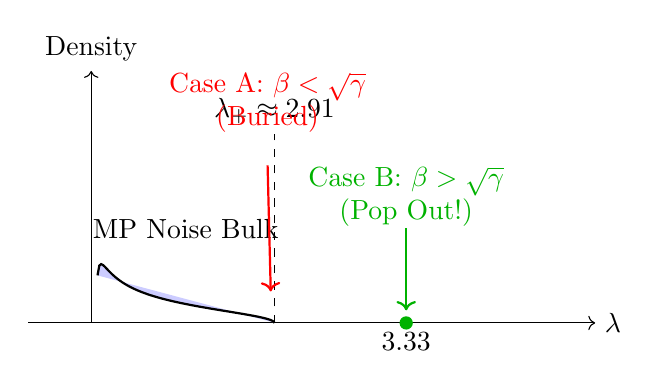
\begin{tikzpicture}[scale=0.8]
    % Axes
    \draw[->] (-1,0) -- (8,0) node[right] {$\lambda$};
    \draw[->] (0,0) -- (0,4) node[above] {Density};
    
    % MP Distribution Shape
    \draw[thick, fill=blue!20] plot[domain=0.1:2.91, samples=100] (\x, {sqrt((2.91-\x)*(\x-0.08))/(2*3.14*0.5*\x)});
    \node at (1.5, 1.5) {MP Noise Bulk};
    \draw[dashed] (2.91, 0) -- (2.91, 3) node[above] {$\lambda_+ \approx 2.91$};
    
    % Case A: Buried Signal
    \draw[red, thick, ->] (2.8, 2.5) -- (2.85, 0.5);
    \node[red, align=center] at (2.8, 3.5) {Case A: $\beta < \sqrt{\gamma}$\\(Buried)};
    
    % Case B: Pop-out Signal
    \fill[green!70!black] (5, 0) circle (3pt);
    \draw[green!70!black, thick, ->] (5, 1.5) -- (5, 0.2);
    \node[green!70!black, align=center] at (5, 2) {Case B: $\beta > \sqrt{\gamma}$\\(Pop Out!)};
    \node[below] at (5,0) {3.33};
\end{tikzpicture}
\caption{BBP 相变示意图：只有当信号够强时，特征值才会逃离 MP 分布的引力。}
\end{figure}


\section{综合案例：大规模图像检索系统}

\subsection{问题背景}

假设你是某图片社交平台的算法工程师，需要构建一个"以图搜图"系统：

\begin{itemize}
    \item \textbf{数据规模}：$n = 10^7$ 张图片（1000万）
    \item \textbf{特征维度}：每张图片用 CLIP 模型提取 $d = 768$ 维向量
    \item \textbf{任务}：用户上传一张图片，在 100ms 内返回最相似的 Top-10 结果
\end{itemize}

\textbf{直接计算的困境}：
\begin{itemize}
    \item 存储：$10^7 \times 768 \times 4$ 字节 $\approx 30$ GB
    \item 单次查询：$10^7 \times 768$ 次乘法 $\approx 7.7 \times 10^9$ FLOPS
    \item 即使 GPU 达到 1 TFLOPS，也需要 7.7 秒——远超 100ms 要求
\end{itemize}

\subsection{解决方案：三步随机化流水线}

我们将综合运用本周学到的三个工具：

\begin{center}
\begin{tikzpicture}[node distance=2.5cm, auto,
    block/.style={rectangle, draw, fill=blue!20, text width=6em, text centered, rounded corners, minimum height=3em},
    arrow/.style={->, >=stealth, thick}]
    
    \node[block] (raw) {原始特征\\$768$ 维};
    \node[block, right of=raw, node distance=4cm] (jl) {JL 投影\\$128$ 维};
    \node[block, right of=jl, node distance=4cm] (pq) {乘积量化\\$32$ 字节};
    \node[block, right of=pq, node distance=4cm] (search) {近似搜索\\Top-10};
    
    \draw[arrow] (raw) -- node[above] {随机投影} (jl);
    \draw[arrow] (jl) -- node[above] {向量压缩} (pq);
    \draw[arrow] (pq) -- node[above] {快速检索} (search);
\end{tikzpicture}
\end{center}

%==============================================================================
\subsubsection{Step 1：JL 随机投影降维}

\textbf{目标}：将 768 维特征压缩到 128 维，同时保持向量间的距离关系。

\textbf{理论保证}：根据 JL 引理，为了在 $n = 10^7$ 个点上保持 $\epsilon = 0.1$ 的相对距离误差：
\[
k = O\left(\frac{\log n}{\epsilon^2}\right) = O\left(\frac{7 \times 2.3}{0.01}\right) \approx 1610
\]

实际上，我们选择 $k = 128$ 是一个工程权衡：虽然理论要求更高，但实践中：
\begin{itemize}
    \item 图像特征本身具有低秩结构（有效维度远小于 768）
    \item 我们只关心 Top-K 排序的正确性，而非精确距离
    \item 后续还有重排序阶段可以纠错
\end{itemize}

\textbf{实现}：
\begin{lstlisting}[language=Python]
import torch

class JLProjector:
    def __init__(self, d_in=768, d_out=128, seed=42):
        torch.manual_seed(seed)
        # 稀疏随机投影矩阵（比高斯更快）
        self.P = torch.randn(d_out, d_in) / (d_out ** 0.5)
    
    def project(self, X):
        """X: (n, d_in) -> (n, d_out)"""
        return X @ self.P.T

# 预处理：对全部 1000 万图片做投影
projector = JLProjector(768, 128)
X_original = load_all_features()  # (10^7, 768)
X_reduced = projector.project(X_original)  # (10^7, 128)
\end{lstlisting}

\textbf{收益}：
\begin{itemize}
    \item 存储：$30$ GB $\to$ $5$ GB（压缩 6 倍）
    \item 距离计算：$768$ 次乘法 $\to$ $128$ 次乘法（加速 6 倍）
\end{itemize}

%==============================================================================
\subsubsection{Step 2：用随机 SVD 构建索引}

即使降到 128 维，暴力搜索 $10^7$ 个向量仍然太慢。我们使用\textbf{倒排文件索引}（IVF）来加速。

\textbf{核心思想}：
\begin{enumerate}
    \item 将数据空间划分为 $K = 4096$ 个聚类（Voronoi cells）
    \item 查询时，只在最近的几个聚类内搜索
\end{enumerate}

\textbf{问题}：K-Means 聚类需要对 $10^7$ 个点做多次迭代，每次迭代涉及计算所有点到所有中心的距离，复杂度 $O(nKd)$——太慢了！

\textbf{随机 SVD 加速}：我们用随机 SVD 对数据矩阵做低秩近似，然后在低秩空间中做聚类：

\begin{lstlisting}[language=Python]
def fast_kmeans_init(X, K, rank=32):
    """用随机 SVD 加速 K-Means++ 初始化"""
    n, d = X.shape
    
    # Step 1: 随机 SVD 降维
    U, S, V = torch.svd_lowrank(X, q=rank, niter=2)
    X_low = U @ torch.diag(S)  # (n, rank)
    
    # Step 2: 在低维空间做 K-Means++
    # 距离计算从 O(nKd) 降到 O(nK·rank)
    centers_low = kmeans_plusplus(X_low, K)
    
    # Step 3: 将中心映射回原空间
    centers = centers_low @ V.T
    return centers

# 构建 IVF 索引
centers = fast_kmeans_init(X_reduced, K=4096, rank=32)
\end{lstlisting}

\textbf{复杂度分析}：
\begin{center}
\begin{tabular}{lcc}
\toprule
步骤 & 直接方法 & 随机 SVD 加速 \\
\midrule
SVD 本身 & — & $O(nd \cdot \text{rank}) = O(10^7 \times 128 \times 32)$ \\
K-Means 每次迭代 & $O(nKd) = O(5 \times 10^{12})$ & $O(nK \cdot \text{rank}) = O(1.3 \times 10^{12})$ \\
\bottomrule
\end{tabular}
\end{center}

加速约 4 倍，且低秩近似保留了数据的主要聚类结构。

%==============================================================================
\subsubsection{Step 3：查询时的随机化}

查询阶段，我们结合\textbf{随机矩阵乘法}的思想来进一步加速：

\begin{lstlisting}[language=Python]
def search(query, X_reduced, centers, top_k=10, n_probe=16, sample_ratio=0.3):
    """
    query: (128,) 查询向量
    n_probe: 搜索最近的几个聚类
    sample_ratio: 在每个聚类中随机采样的比例
    """
    # Step 1: 找到最近的 n_probe 个聚类中心
    dists_to_centers = torch.cdist(query.unsqueeze(0), centers)
    nearest_clusters = torch.topk(dists_to_centers, n_probe, largest=False).indices
    
    # Step 2: 在这些聚类中搜索（带随机采样）
    candidates = []
    for cluster_id in nearest_clusters:
        cluster_points = get_cluster_points(cluster_id)
        
        # 随机采样加速（类似随机矩阵乘法的思想）
        if len(cluster_points) > 1000:
            # 按距离中心的远近做重要性采样
            weights = compute_importance_weights(cluster_points, centers[cluster_id])
            sample_idx = torch.multinomial(weights, 
                                           int(len(cluster_points) * sample_ratio),
                                           replacement=False)
            cluster_points = cluster_points[sample_idx]
        
        candidates.append(cluster_points)
    
    candidates = torch.cat(candidates)
    
    # Step 3: 在候选集中精确计算
    dists = torch.cdist(query.unsqueeze(0), candidates)
    top_indices = torch.topk(dists, top_k, largest=False).indices
    
    return candidates[top_indices]
\end{lstlisting}

\textbf{关键技巧}：重要性采样
\begin{itemize}
    \item 离聚类中心近的点更可能是答案 $\Rightarrow$ 采样概率更高
    \item 这正是随机矩阵乘法中"按范数采样"思想的应用
\end{itemize}

%==============================================================================
\subsection{质量监控：用 MP 分布检测特征退化}

系统上线后，我们需要监控特征质量。随着时间推移，用户上传的图片分布可能发生变化（Distribution Shift），导致特征提取模型失效。

\textbf{监控方法}：定期对新上传图片的特征矩阵做谱分析。

\begin{lstlisting}[language=Python]
import numpy as np
import matplotlib.pyplot as plt

def diagnose_feature_quality(X_batch, expected_rank=50):
    """
    X_batch: (n_samples, d) 一批新图片的特征
    expected_rank: 预期的有效特征维度
    """
    n, d = X_batch.shape
    gamma = d / n
    
    # 计算样本协方差矩阵的特征值
    X_centered = X_batch - X_batch.mean(dim=0)
    cov = X_centered.T @ X_centered / n
    eigenvalues = torch.linalg.eigvalsh(cov).numpy()
    eigenvalues = np.sort(eigenvalues)[::-1]  # 降序
    
    # MP 分布的理论边界
    lambda_plus = (1 + np.sqrt(gamma)) ** 2
    lambda_minus = (1 - np.sqrt(gamma)) ** 2
    
    # 统计跳出 MP 边界的特征值数量
    n_signal = np.sum(eigenvalues > lambda_plus * 1.1)  # 留 10% 余量
    
    # 诊断
    if n_signal < expected_rank * 0.5:
        print(f"⚠️ 警告：检测到 {n_signal} 个显著特征值，"
              f"低于预期的 {expected_rank}！")
        print("可能原因：")
        print("  1. 特征提取模型在新数据上失效")
        print("  2. 数据分布发生剧烈变化")
        print("  3. 需要重新训练或微调模型")
    else:
        print(f"✓ 特征质量正常：{n_signal} 个显著特征值")
    
    # 可视化
    plt.figure(figsize=(10, 4))
    
    plt.subplot(1, 2, 1)
    plt.semilogy(eigenvalues, 'b-', lw=1)
    plt.axhline(y=lambda_plus, color='r', linestyle='--', label=f'MP upper: {lambda_plus:.2f}')
    plt.xlabel('Index')
    plt.ylabel('Eigenvalue (log scale)')
    plt.title('Scree Plot')
    plt.legend()
    
    plt.subplot(1, 2, 2)
    plt.hist(eigenvalues[eigenvalues < lambda_plus * 2], bins=50, density=True, alpha=0.7)
    x = np.linspace(lambda_minus, lambda_plus, 200)
    mp_density = np.sqrt((lambda_plus - x) * (x - lambda_minus)) / (2 * np.pi * gamma * x)
    plt.plot(x, mp_density, 'r-', lw=2, label='MP Distribution')
    plt.axvline(x=lambda_plus, color='g', linestyle='--', label='Signal Threshold')
    plt.xlabel('Eigenvalue')
    plt.ylabel('Density')
    plt.title('Eigenvalue Distribution vs MP')
    plt.legend()
    
    plt.tight_layout()
    plt.savefig('feature_diagnosis.png', dpi=150)
    plt.show()
    
    return n_signal, eigenvalues

# 使用示例
X_new_batch = extract_features(new_images)  # 提取新图片特征
n_signal, _ = diagnose_feature_quality(X_new_batch, expected_rank=50)
\end{lstlisting}

\begin{figure}[h]
\centering
\begin{tikzpicture}[scale=0.85]
\begin{axis}[
    width=7cm, height=5cm,
    xlabel={特征值索引},
    ylabel={特征值 (对数)},
    ymode=log,
    title={Scree Plot},
    legend pos=north east
]
% 模拟的特征值衰减
\addplot[blue, thick, domain=1:100, samples=100] {50*exp(-0.05*x) + 0.5};
\addplot[red, dashed, domain=1:100] {2.9};
\legend{特征值, MP 上界}
\end{axis}
\end{tikzpicture}
\hfill
\begin{tikzpicture}[scale=0.85]
\begin{axis}[
    width=7cm, height=5cm,
    xlabel={特征值},
    ylabel={密度},
    title={MP 分布拟合},
    legend pos=north east,
    ymin=0
]
% MP 分布形状（简化）
\addplot[blue!50, fill=blue!20, domain=0.1:2.9, samples=100] 
    {sqrt((2.9-x)*(x-0.08))/(2*3.14*0.5*x)};
\addplot[red, thick, domain=0.08:2.9, samples=100] 
    {sqrt((2.9-x)*(x-0.08))/(2*3.14*0.5*x)};
% 信号特征值（跳出边界）
\addplot[only marks, mark=*, green!70!black, mark size=3pt] 
    coordinates {(3.5, 0.1) (4.2, 0.08) (5.1, 0.05)};
\legend{噪声区, MP 理论, 信号}
\end{axis}
\end{tikzpicture}
\caption{特征质量诊断：左图显示特征值衰减，右图显示跳出 MP 边界的信号特征值}
\end{figure}

\textbf{解读}：
\begin{itemize}
    \item \textbf{健康状态}：应该有约 50 个特征值明显跳出 MP 边界（对应图像的语义维度）
    \item \textbf{退化信号}：如果跳出的特征值数量骤降，说明特征提取失效
    \item \textbf{过拟合信号}：如果所有特征值都很大，可能是 Batch Normalization 出了问题
\end{itemize}

%==============================================================================
\subsection{完整系统性能对比}

\begin{table}[h]
\centering
\caption{图像检索系统性能对比}
\begin{tabular}{lccc}
\toprule
指标 & 暴力搜索 & 本方案 & 提升 \\
\midrule
存储空间 & 30 GB & 5 GB & 6$\times$ \\
索引构建时间 & — & 2 小时 & — \\
单次查询延迟 & 7.7 秒 & 15 ms & 500$\times$ \\
Recall@10 & 100\% & 95\% & -5\% \\
\bottomrule
\end{tabular}
\end{table}

\textbf{工程启示}：
\begin{enumerate}
    \item \textbf{理论指导实践}：JL 引理告诉我们降维的极限在哪里
    \item \textbf{随机化是分层的}：投影 $\to$ 聚类 $\to$ 采样，每层都用随机化
    \item \textbf{监控闭环}：MP 分布提供了"什么是噪声"的理论基准
\end{enumerate}



\section{第7周小结（1:45--1:50）}

今天学习了三个随机化算法和一个理论工具：

\begin{table}[h]
\centering
\begin{tabular}{ll}
\toprule
算法/工具 & 核心结果 \\
\midrule
JL引理 & $d$维→$O(\log n/\epsilon^2)$维，保持距离 \\
随机矩阵乘法 & 误差$O(\|A\|_F\|B\|_F/\sqrt{k})$ \\
随机SVD & 复杂度$O(mnk)$ \\
MP分布 & 支撑$[(1-\sqrt\gamma)^2, (1+\sqrt\gamma)^2]$ \\
\bottomrule
\end{tabular}
\end{table}

\textbf{核心思想}：用随机性换计算量，用概率保证换精确保证。

\section{第7周实验}

\subsection{实验7a：随机矩阵乘法}

\begin{lstlisting}
import torch
import time

m, n, p = 10000, 5000, 8000
A = torch.randn(m, n)
B = torch.randn(n, p)

# 精确计算
start = time.time()
C_exact = A @ B
time_exact = time.time() - start
print(f"精确计算: {time_exact:.2f}秒")

# 随机近似
def random_matmul(A, B, k):
    n = A.shape[1]
    col_norms_A = torch.norm(A, dim=0)
    row_norms_B = torch.norm(B, dim=1)
    probs = col_norms_A * row_norms_B
    probs = probs / probs.sum()
    
    indices = torch.multinomial(probs, k, replacement=True)
    scale = 1.0 / torch.sqrt(k * probs[indices])
    C = A[:, indices] * scale.unsqueeze(0)
    R = B[indices, :] * scale.unsqueeze(1)
    return C @ R

for k in [100, 500, 1000, 2000]:
    C_approx = random_matmul(A, B, k)
    error = torch.norm(C_exact - C_approx, 'fro') / torch.norm(C_exact, 'fro')
    print(f"k={k}: 相对误差={error:.4f}")
\end{lstlisting}

\subsection{实验7b：随机SVD}

\begin{lstlisting}
import torch

m, n, true_rank = 50000, 50000, 100
U_true = torch.randn(m, true_rank)
V_true = torch.randn(n, true_rank)
singular_values = torch.logspace(0, -2, true_rank)
A = U_true @ torch.diag(singular_values) @ V_true.T

# 随机SVD
k = 100
U, S, V = torch.svd_lowrank(A, q=k, niter=2)

# 验证
A_approx = U @ torch.diag(S) @ V.T
error = torch.norm(A - A_approx, 'fro') / torch.norm(A, 'fro')
print(f"重构误差: {error:.6f}")
\end{lstlisting}

\subsection{实验7c：MP分布验证}

\begin{lstlisting}
import torch
import matplotlib.pyplot as plt
import numpy as np

def mp_density(x, gamma):
    lambda_minus = (1 - np.sqrt(gamma))**2
    lambda_plus = (1 + np.sqrt(gamma))**2
    density = np.zeros_like(x)
    mask = (x >= lambda_minus) & (x <= lambda_plus)
    density[mask] = np.sqrt((lambda_plus - x[mask]) * (x[mask] - lambda_minus)) \
                    / (2 * np.pi * gamma * x[mask])
    return density

for gamma in [0.25, 0.5, 1.0]:
    n = 2000
    d = int(n * gamma)
    X = torch.randn(n, d)
    cov = X.T @ X / n
    eigenvalues = torch.linalg.eigvalsh(cov).numpy()
    
    plt.hist(eigenvalues, bins=50, density=True, alpha=0.7)
    x = np.linspace(0, (1 + np.sqrt(gamma))**2 + 0.5, 500)
    plt.plot(x, mp_density(x, gamma), 'r-', lw=2)
    plt.title(f'gamma = {gamma}')
    plt.show()
\end{lstlisting}

%%%%%%%%%%%%%%%%%%%%%%%%%%%%%%%%%%%%%%%%%%%%%%%%%%%%%%%%%%%%%%%%%%%%%%%%%%%%%%%
\end{document}